% PAKETE UND DOKUMENTKONFIGURATION
\documentclass[11pt, a4paper]{article}

% Encoding für Umlaute
\usepackage[utf8]{inputenc}
\usepackage[T1]{fontenc}

% Silbentrennung
\usepackage[ngerman]{babel}

% erweiterte Matheumgebungen
\usepackage{amsmath}

% Braket Notation
\usepackage{braket}

% zusätzliche mathematische Schriftarten
\usepackage{amsfonts}

% verschiedene mathematische Symbole
\usepackage{amssymb}

% Einheiten setzen z.B. \SI{10}{\kilo\gram\meter\per\second\squared}
% Fehler: \SI{10 +- 0,2e-4}{\metre}
\usepackage{siunitx}
\sisetup{
  output-decimal-marker={,},
  separate-uncertainty
}

% Randbreiten
\usepackage[left=3.5cm,right=3.5cm,top=3cm,bottom=3cm,twoside]{geometry}

% Bilder einfügen
\usepackage{graphicx}

% Verweise innerhalb des Dokuments
\usepackage{hyperref}
\hypersetup{
	colorlinks = true,
	allcolors = {black}
}

% bessere Tabellenlayouts
\usepackage{booktabs}

% Seitenlayout (Kopfzeile)
\usepackage{fancyhdr}

% Float Barriers
\usepackage{placeins}

% Pakete für gedrehte Subfigures
\usepackage{caption}
\usepackage{subcaption}
\usepackage{rotating}

% Manuelle Silbentrennung
\hyphenation{Halb-werts-brei-te Fa-bry-Pé-rot-E-ta-lon Zee-man-E-ffekt}

% Tiefe des Inhaltsverzeichnisses (Level: 1 sections, 2 subsections,
% 3 subsubsections)
\setcounter{tocdepth}{3}

% FANCYHDR SETUP
\pagestyle{fancy}
\fancyhead[EL,OR]{\thepage}
\fancyhead[ER]{\leftmark}
\fancyhead[OL]{\rightmark}

\renewcommand{\sectionmark}[1]{
\markboth{Abschnitt \thesection{}: #1}{\thesection{} #1}
}
\renewcommand{\subsectionmark}[1]{
\markright{\thesubsection{} #1}
}

% DOKUMENTINFORMATIONEN
\title{P401 \\ Elektronische Übergänge in Atomen}

\author{Christopher Deutsch\footnote{christopher.deutsch@uni-bonn.de} \and Christian Bespin\footnote{christian.bespin@uni-bonn.de}}

\date{\today}

\begin{document}

\begin{titlepage}

\maketitle

% DURCHFÜHRUNGSDATUM UND ASSISTENT
\begin{center}
\begin{tabular}{l r}
Durchführung: & 17./18. November 2014 \\
Gruppe: & $\alpha$ 2 \\
Assistent: & Jens-Peter Thiry
\end{tabular}
\end{center}

% ZUSAMMENFASSUNG
\begin{abstract}
\noindent
% Text
\end{abstract}

\end{titlepage}

% INHALTSVERZEICHNIS
\tableofcontents
% Neue Seite nach TOC
\newpage

% INHALT VERSUCHSPROTOKOLL

\section{Grundlagen / Theorie}

\subsection{Zeeman-Effekt}

Der Zeeman-Effekt beschreibt die Aufspaltung entarteter Energieniveaus unter Einfluss eines äußeren Magnetfeldes.
In diesem Versuch wollen wir uns dabei auf den normalen Zeeman-Effekt beschränken; dieser gilt für Atome, deren Gesamtspin gleich $0$ ist und so nur Drehimpulse $\vec{L}$ zum Gesamtdrehimpuls $\vec{J}=\vec{L}+\vec{S}$ beitragen.

\subsubsection{Verhalten von Atomen in äußeren Feldern}
\label{sec:zeemaneffekt}

Aus der Lösung der Schrödingergleichung für ein Elektron im Coulombpotenzial eines Kerns folgt, dass es nur diskrete Energiewerte annehmen kann.
Diese werden über die so genannte Hauptquantenzahl $n$ bestimmt.
Zusätzlich dazu kann man weitere Quantenzahlen definieren, wir beschränken uns hier auf die Quantenzahlen $l$ für den Drehimpuls, $s$ für den Spin und $j$ für den Gesamtdrehimpuls aus $\ell$ und $s$.
Für $n$ und $l$ gilt $n=1, 2, 3 \dots$ und $l=0, 1, 2 \dots n-1$, wobei die Werte für $l$ häufig mit den Buchstaben s, p, d, f, g $\dots$ (ab f alphabetisch) identifiziert werden.
Die möglichen Werte von $j=\ell+s$ ergeben sich mit dem Elektronenspin $s=\pm1/2$ entsprechend.
Da es nicht möglich ist, zwei Komponenten $L_i, L_j$ des Drehimpulses gleichzeitig zu bestimmen (folgt aus Kommutatorrelation), erhält man bei einer Messung von $|\vec{L}|$ und $L_z$, welche durchgeführt werden kann, eine weitere Quantenzahl $m_l$ (analog erhält für $|\vec{J}|$ und $J_z$ $m_j$). Sie beschreibt im Vektormodell anschaulich die Projektion von $\vec{L}$ auf die $z$-Achse.
Dabei gilt für die Eigenwerte der Operatoren $\hat{L}^2$ und $\hat{L}_z$:
\begin{align*}
|\vec{L}|&=\hbar\sqrt{l(l+1)}\\
l_z&=\hbar m_l
\end{align*}
Ausgehend hiervon betrachtet man den Einfluss der Bahndrehimpulse auf die Energieniveaus im Atom.
Dazu verwenden wir das Vektormodell, in dem der Bahndrehimpuls als Vektor geschrieben werden kann und woraus sich Wechselwirkungen im Atom einfach beschreiben lassen.
Ein Elektron mit Bahndrehimpuls $\vec{\ell}$ entspricht dann im klassischen Bild einem Kreisstrom.
Dieser führt zu einem magnetischen Dipolmoment, welches gegeben ist durch:
\begin{align*}
	\vec{\mu}_\ell = - \frac{\mu_\mathrm{B}}{\hbar} \vec{\ell}
\end{align*}
Wobei das Bohr'sche Magneton definiert ist als:
\begin{align*}
	\mu_\mathrm{B} = \frac{e \hbar}{2 m_e}
\end{align*}
Die potentielle Energie eines magnetischen Dipols im externen magnetischen Feld $B$ ist gegeben durch:
\begin{align*}
	E_\mathrm{pot} = - \vec{\mu} \cdot \vec{B}
\end{align*}
Damit kommt es zu einer Energieverschiebung $\Delta E$ der Niveaus aufgrund der potentiellen Energie des Dipols im Magnetfeld:
\begin{align*}
	\Delta E = \frac{\mu_\mathrm{B}}{\hbar} \left( \vec{\ell} \cdot \vec{B} \right)
\end{align*}
Wählt man $\vec{B} = (0,0,B_z)$ und dementsprechend die z-Achse als Quantisierungsachse des Drehimpulses, so folgt $\ell_z = \hbar m_\ell$ aus der magnetischen Quantenzahl $m_\ell$ und die Energieverschiebung ergibt sich zu:
\begin{align}
	\Delta E = \mu_\mathrm{B} m_\ell B_z
	\label{eq:normaler_zeeman}
\end{align}
Somit wird für feste Drehimpulsquantenzahl $\ell$ die Entartung des zugehörigen Energieniveaus aufgehoben, da sich dieses in $(2\ell + 1)$ Niveaus aufspaltet.
\begin{figure}[h]
\centering
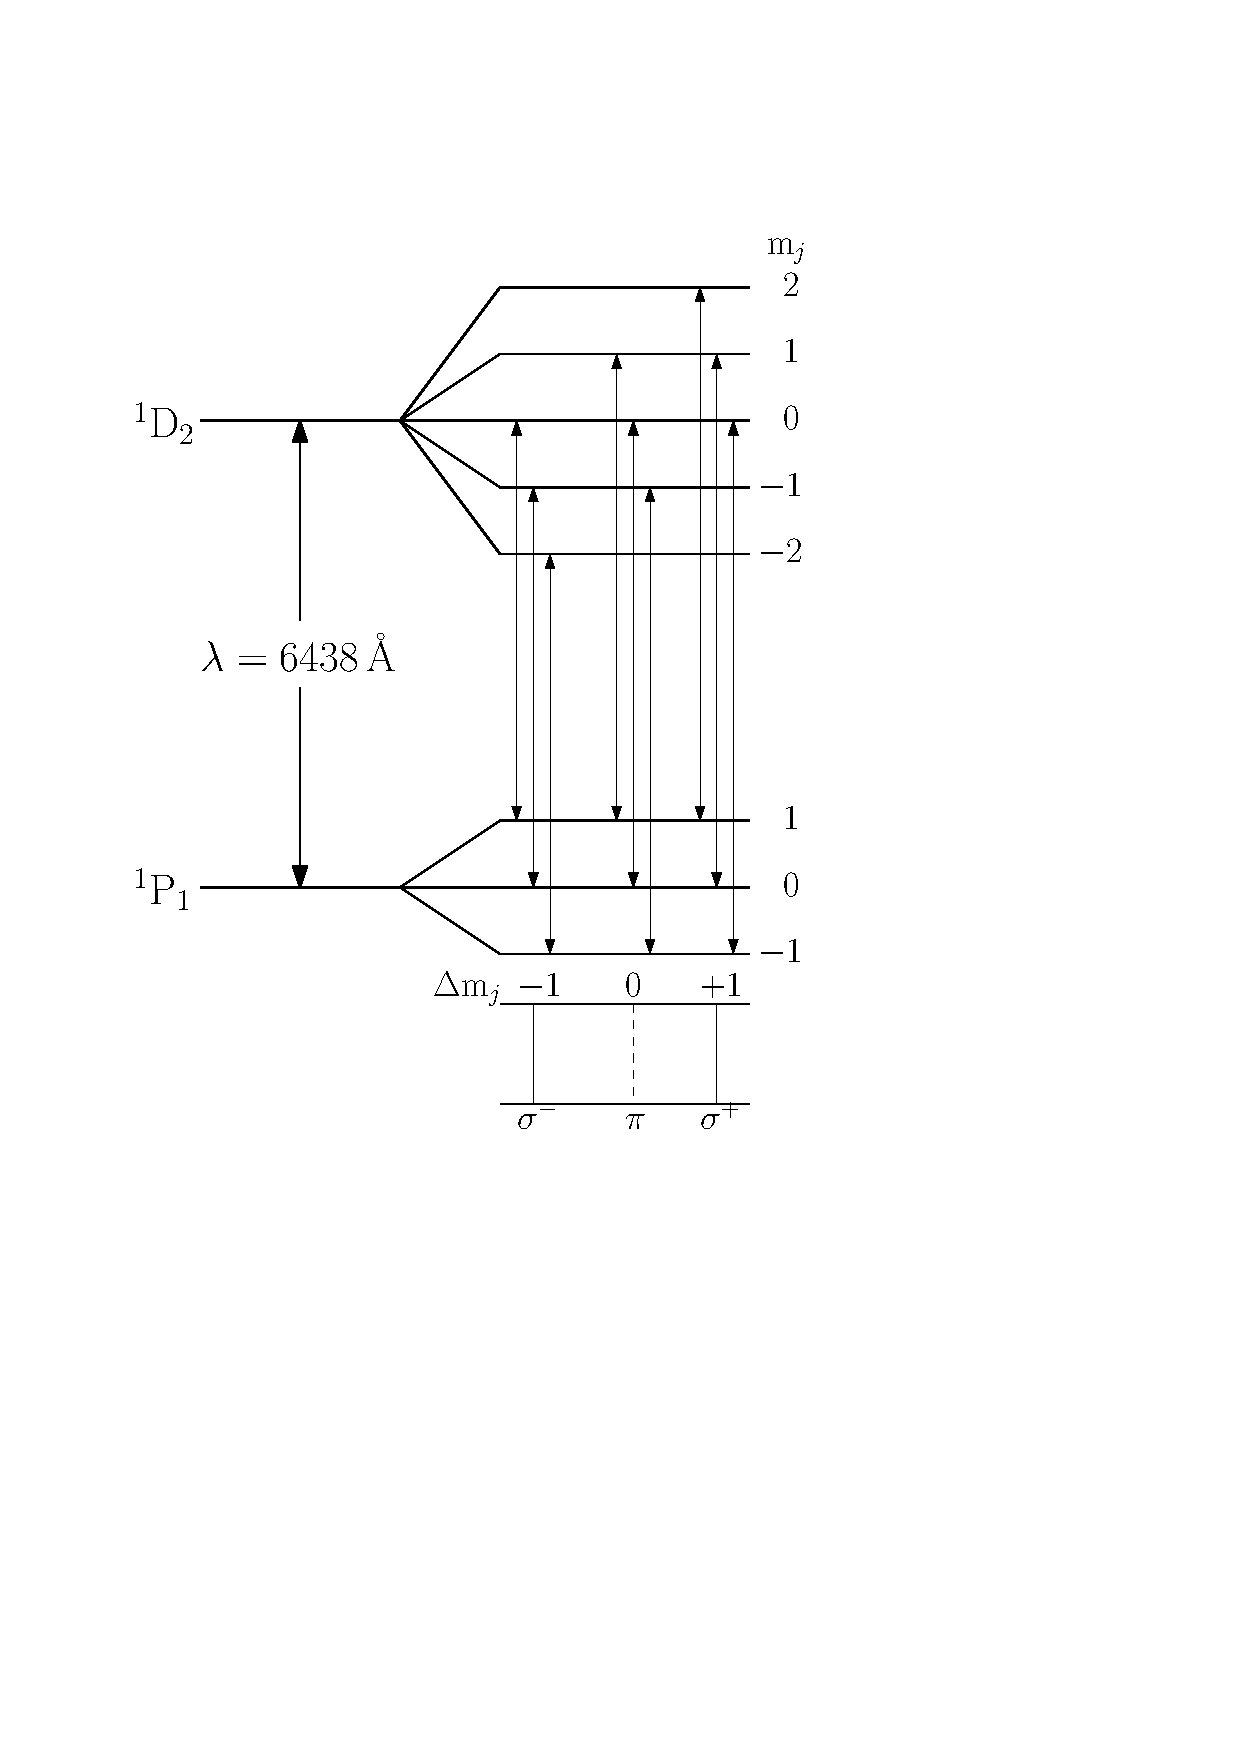
\includegraphics[width=0.4\textwidth]{./figures/termschema_cadmium.pdf}
\caption{Übergang von $^1$D$_2$ nach $^1$P$_1$ in der fünften Schale in Cadmium}
\label{fig:termschema_cadmium}
\end{figure}
Im Gegensatz dazu wird beim anormalen Zeeman-Effekt das magnetische Moment aufgrund des Elektronenspins beachtet.
Dies führt dazu, dass das magnetische Moment des Elektrons gegeben ist durch:
\begin{align}
\vec{\mu} = -\frac{\mu_\mathrm{B}}{\hbar} \left( \vec{l} + g_s \vec{s} \right)
\label{eq:magmom_spin}
\end{align}
Zur Beschreibung der Energieverschiebung ist hier die Kopplung von Spin und Bahndrehimpuls $\vec{j} = \vec{\ell} + \vec{s}$ nötig.
Da $g_s \approx 2$ ist, ist das magnetische Moment des Elektrons nicht parallel zum Gesamtdrehimpuls $\vec{j}$ und präzediert um diesen.
Daher muss ein effektives magnetisches Moment als Projektion von $\vec{\mu}$ auf $\vec{j}$ berechnet werden, was zu dem effektiven Moment:
\begin{align*}
	\vec{\mu}_\mathrm{eff} = - g_j \frac{\mu_\mathrm{B}}{\hbar} \vec{j} 
\end{align*}
führt.
Dabei ist der sogenannte Landé-Faktor $g_j$ abhängig von den Quantenzahlen $l,s,j$ des Zustandes.
Damit folgt analog zum normalen Zeeman-Effekt:
\begin{align}
	\Delta E = \mu_\mathrm{B} g_j m_j B_z
\end{align}

\subsubsection{Auswahlregeln}
\label{sec:auswahlregeln}
Die Auswahlregeln für elektrische Dipolübergänge erhält man durch Berechnung der Übergangswahrscheinlichkeit vom Anfangszustand $|i\rangle$ in den Endzustand $|f\rangle$ durch Fermis "`Goldene Regel"':
\begin{align*}
	\lambda_{i\rightarrow f} = \frac{2 \pi}{\hbar} | \braket{f|H^\prime|i} |^2 \rho(E_\mathrm{f})
\end{align*}
Dabei ist der Störhamiltonian $H^\prime$ gegeben durch die Störung der Energie aufgrund der Kopplung von einem externen elektrischen Feld $\vec{E}$ an das elektrische Dipolmoment $\vec{p}$ des Zustandes:
\begin{align*}
	H^\prime = - \vec{p} \cdot \vec{E}
\end{align*}
Kennzeichnend dafür, ob ein Übergang erlaubt ist, ist das jeweilige Matrixelement des Störhamiltonians.
Man erhält somit folgende Auswahlregeln aus den nicht verschwindenden Matrixelementen:
\begin{itemize}
	\item $\Delta n$ beliebig
	\item $\Delta \ell = \pm 1$ \quad (Drehimpulserhaltung mit $s_\mathrm{Photon} = \pm \hbar$)
	\item $\Delta s = 0$ \quad (reine Spin-Flips sind nicht möglich)
	\item $\Delta j = 0, \pm 1$, außer $j_i=0 \rightarrow j_f=0$
	\item $\Delta m_j = 0, \pm 1$
\end{itemize}
($n$: Hauptquantenzahl, $\ell$: Drehimpulsquantenzahl, $s$: Spinquantenzahl, $j$: Gesamtdrehimpulsquantenzahl, $m_j$: magnetische Quantenzahl)

Mit diesen Auswahlregeln folgen die Übergänge für Cadmium aus Abbildung \ref{fig:termschema_cadmium}.
Anzumerken ist, dass es sich dabei um den normalen Zeeman-Effekt handelt und dadurch die Aufspaltung der P-Schale ($\ell = 1$) den gleichen Abstand hat, wie die der D-Schale ($\ell = 2$).
Dadurch kommt es hier zu insgesamt drei Übergängen, mit unterschiedlichen Energien.
Im Vergleich dazu liefert der anormaler Zeeman-Effekt mehrere Übergänge mit unterschiedlicher Energie, da sich die Energieniveaus aufgrund der Abhängigkeit vom Landé-Faktor in den jeweiligen Schalen nicht äquidistant aufspalten.

Die Elektronenkonfiguration des in diesem Versuch verwendeten Cadmiums ist [Kr] $4$d$^{10} 5$s$^2$, was nur abgeschlossene Schalen entspricht und daher hat das Atom einen Gesamtspin $S=0$, weswegen wir nur den normalen Zeeman-Effekt beobachten.

\subsubsection{Fabry-Pérot-Etalon}
Das Fabry-Pérot-Etalon besteht aus einer transparenten Platte, welche beidseitig von Luft umgeben ist.
Trifft eine elektromagnetische Welle unter dem Winkel $\alpha$ auf das Etalon, so wird diese an beiden Grenzfläche gemäß des Reflexionskoeffizienten\footnote{Der Reflexionskoeffizient beschreibt die Änderung der Amplitude der elektromagnetischen Welle bei Reflexion an der Grenzfläche. Das Verhältnis der Intensitäten ist durch den Reflexionsgrad $R = r^2$ gegeben.} $r$ reflektiert und zum Teil transmittiert.
Dies führt dazu, dass die Welle innerhalb des Etalons sehr oft hin- und her reflektiert wird und es somit auf Transmissionsseite der Platte zur Vielstrahlinterferenz der transmittierten Strahlen kommt.
Da in diesem Versuch das Fabry-Pérot-Etalon in Transmission betrieben wird, wollen wir uns auf diesen Fall beschränken.
\begin{figure}[h]
	\centering
	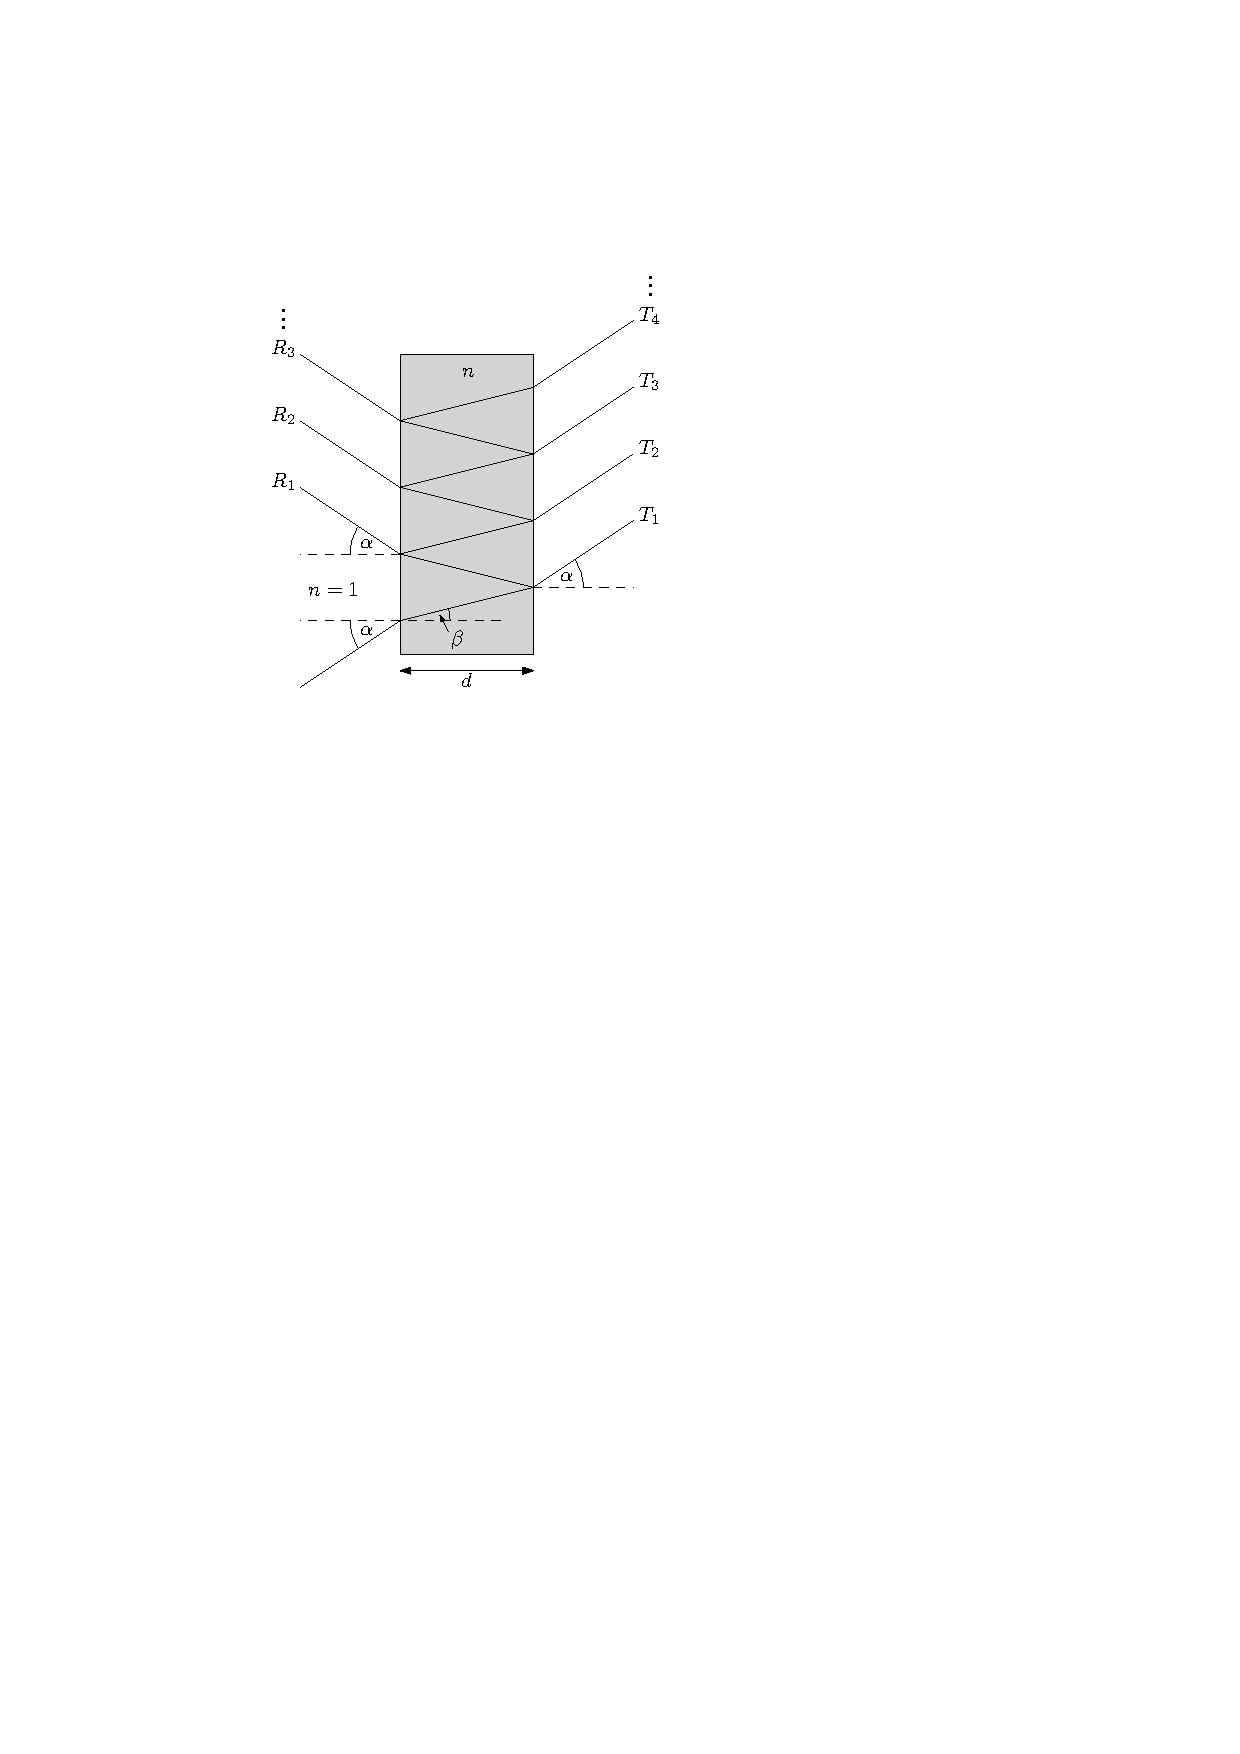
\includegraphics[width=0.5\textwidth]{./figures/fabry_perot.pdf}
	\caption{Berechnung der optischen Weglänge des Fabry-Pérot-Etalons}
	\label{fig:fabry_perot}
\end{figure}
Um die Bedingung für konstruktive Interferenz zu erhalten, muss zunächst der optische Gangunterschied zweier benachbarter Strahlen berechnet werden.
Gemäß Abbildung \ref{fig:fabry_perot} ist dieser gegeben durch:
\begin{align*}
	\Delta s = \frac{2 n d}{\cos(\beta)} - 2 n d \sin(\alpha) \tan(\beta)
\end{align*}
Mit dem Brechungsgesetz $\sin(\alpha) = n \sin(\beta)$ folgt:
\begin{align*}
	\Delta s = 2 d \sqrt{n^2 - \sin^2(\alpha)}
\end{align*}
Damit zwei benachbarte Strahlen nach der Transmission in Phase sind, muss deren Phasendifferenz $\Delta \varphi$ ein ganzzahliges Vielfaches von $2\pi$ sein:
\begin{align*}
	\Delta \varphi = k \cdot \Delta s = \frac{2\pi}{\lambda} \Delta s = 2 \pi \cdot m \quad \text{mit } m \in \mathbb{Z}
\end{align*}
Damit ist die Bedingung für ein Maximum der Transmission:
\begin{align}
	m \lambda = 2 d \sqrt{n^2 - \sin^2(\alpha)}
	\label{eq:interferenzbedingung}
\end{align}
Führt man die Berechnung der Transmission unter Beachtung der Amplituden und Phasen der einzelnen Teilwellen durch, so erhält man für den Transmissionsgrad $T = I_\mathrm{T} / I_0$:
\begin{align*}
	T = \frac{1}{1 + F \sin^2(\Delta \varphi / 2)}
\end{align*}
wobei man den Finesse-Koeffizienten
\begin{align*}
	F = \left( \frac{2 r}{1 - r^2} \right)^2
\end{align*}
definiert.\footnote{Quelle: Vorlesung Optik und Wellenmechanik (WS 2013/2014) bei Prof. Dr. Linden}
\begin{figure}[h]
	\centering
	\scalebox{0.9}{
	% GNUPLOT: LaTeX picture with Postscript
\begingroup
  \makeatletter
  \providecommand\color[2][]{%
    \GenericError{(gnuplot) \space\space\space\@spaces}{%
      Package color not loaded in conjunction with
      terminal option `colourtext'%
    }{See the gnuplot documentation for explanation.%
    }{Either use 'blacktext' in gnuplot or load the package
      color.sty in LaTeX.}%
    \renewcommand\color[2][]{}%
  }%
  \providecommand\includegraphics[2][]{%
    \GenericError{(gnuplot) \space\space\space\@spaces}{%
      Package graphicx or graphics not loaded%
    }{See the gnuplot documentation for explanation.%
    }{The gnuplot epslatex terminal needs graphicx.sty or graphics.sty.}%
    \renewcommand\includegraphics[2][]{}%
  }%
  \providecommand\rotatebox[2]{#2}%
  \@ifundefined{ifGPcolor}{%
    \newif\ifGPcolor
    \GPcolortrue
  }{}%
  \@ifundefined{ifGPblacktext}{%
    \newif\ifGPblacktext
    \GPblacktexttrue
  }{}%
  % define a \g@addto@macro without @ in the name:
  \let\gplgaddtomacro\g@addto@macro
  % define empty templates for all commands taking text:
  \gdef\gplbacktext{}%
  \gdef\gplfronttext{}%
  \makeatother
  \ifGPblacktext
    % no textcolor at all
    \def\colorrgb#1{}%
    \def\colorgray#1{}%
  \else
    % gray or color?
    \ifGPcolor
      \def\colorrgb#1{\color[rgb]{#1}}%
      \def\colorgray#1{\color[gray]{#1}}%
      \expandafter\def\csname LTw\endcsname{\color{white}}%
      \expandafter\def\csname LTb\endcsname{\color{black}}%
      \expandafter\def\csname LTa\endcsname{\color{black}}%
      \expandafter\def\csname LT0\endcsname{\color[rgb]{1,0,0}}%
      \expandafter\def\csname LT1\endcsname{\color[rgb]{0,1,0}}%
      \expandafter\def\csname LT2\endcsname{\color[rgb]{0,0,1}}%
      \expandafter\def\csname LT3\endcsname{\color[rgb]{1,0,1}}%
      \expandafter\def\csname LT4\endcsname{\color[rgb]{0,1,1}}%
      \expandafter\def\csname LT5\endcsname{\color[rgb]{1,1,0}}%
      \expandafter\def\csname LT6\endcsname{\color[rgb]{0,0,0}}%
      \expandafter\def\csname LT7\endcsname{\color[rgb]{1,0.3,0}}%
      \expandafter\def\csname LT8\endcsname{\color[rgb]{0.5,0.5,0.5}}%
    \else
      % gray
      \def\colorrgb#1{\color{black}}%
      \def\colorgray#1{\color[gray]{#1}}%
      \expandafter\def\csname LTw\endcsname{\color{white}}%
      \expandafter\def\csname LTb\endcsname{\color{black}}%
      \expandafter\def\csname LTa\endcsname{\color{black}}%
      \expandafter\def\csname LT0\endcsname{\color{black}}%
      \expandafter\def\csname LT1\endcsname{\color{black}}%
      \expandafter\def\csname LT2\endcsname{\color{black}}%
      \expandafter\def\csname LT3\endcsname{\color{black}}%
      \expandafter\def\csname LT4\endcsname{\color{black}}%
      \expandafter\def\csname LT5\endcsname{\color{black}}%
      \expandafter\def\csname LT6\endcsname{\color{black}}%
      \expandafter\def\csname LT7\endcsname{\color{black}}%
      \expandafter\def\csname LT8\endcsname{\color{black}}%
    \fi
  \fi
  \setlength{\unitlength}{0.0500bp}%
  \begin{picture}(7200.00,5040.00)%
    \gplgaddtomacro\gplbacktext{%
      \csname LTb\endcsname%
      \put(946,374){\makebox(0,0)[r]{\strut{} 0}}%
      \put(946,1254){\makebox(0,0)[r]{\strut{} 0.2}}%
      \put(946,2134){\makebox(0,0)[r]{\strut{} 0.4}}%
      \put(946,3015){\makebox(0,0)[r]{\strut{} 0.6}}%
      \put(946,3895){\makebox(0,0)[r]{\strut{} 0.8}}%
      \put(946,4775){\makebox(0,0)[r]{\strut{} 1}}%
      \put(176,2574){\rotatebox{-270}{\makebox(0,0){\strut{}Transmissionsgrad}}}%
      \put(3940,154){\makebox(0,0){\strut{}Wellenl\"ange $\lambda$}}%
      \put(3940,4665){\makebox(0,0){\strut{}}}%
    }%
    \gplgaddtomacro\gplfronttext{%
    }%
    \gplbacktext
    \put(0,0){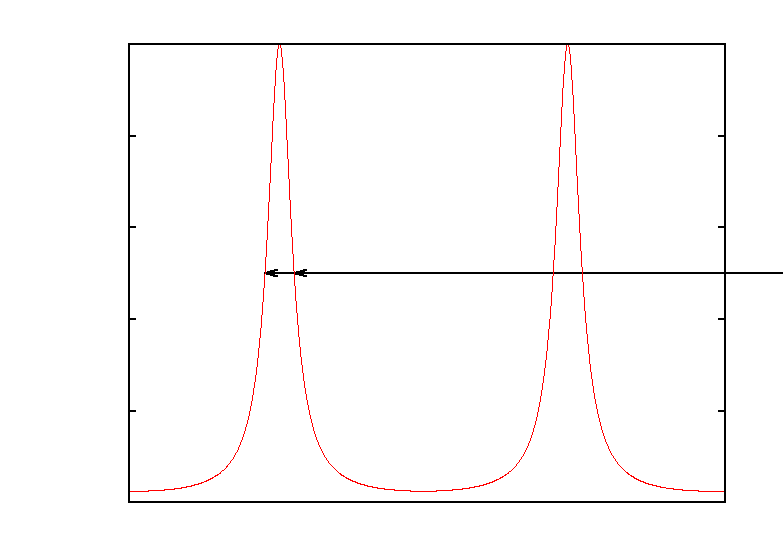
\includegraphics{./fabry_perot_transmission}}%
    \gplfronttext
  \end{picture}%
\endgroup
}
	\caption{Transmission am Fabry-Pérot-Etalon in Abhängigkeit der Wellenlänge und Erklärung zur Halbwertsbreite $\delta\lambda$ und freiem Spektralbereich $\Delta\lambda$}
	\label{fig:fabry_transmission}
\end{figure}
Zwei wichtige Kenngrößen des Fabry-Pérot-Etalons sind die Halbwertsbreite des Transmissionsmaximums $\delta \lambda$, sowie der freie Spektralbereich $\Delta \lambda$, welcher als Abstand zweier Transmissionsmaxima definiert ist.
Mit diesen zwei Größen definiert man die Finesse $\mathcal{F}$ des Etalons \cite{hecht}:
\begin{align}
	\mathcal{F} = \frac{\Delta \lambda}{\delta \lambda} = \frac{\pi \sqrt{F}}{2} = \frac{\pi r}{1 - r^2}
	\label{eq:finesse}
\end{align}

Das Auflösungsvermögen $\mathcal{R}$ ist definiert als das Verhältnis der Wellenlänge $\lambda$ zur Wellenlängendifferenz von zwei gerade noch auflösbaren Linien.
Gerade noch auflösbar heißt dabei, dass das Rayleigh-Kriterium erfüllt ist, welches besagt, dass der Abstand der beiden Intensitätsmaxima genau der Halbwertsbreite des Intensitätsverlaufs entspricht.
Damit folgt mit der Halbwertsbreite $\delta \lambda$ der Maxima des Fabry-Pérot-Etalons \cite{hecht}:
\begin{align}
	\mathcal{R} = \frac{\lambda}{\delta \lambda} = \mathcal{F} \cdot m
	\label{eq:aufloesung}
\end{align}

\subsubsection{Natürliche Linienbreite und Linienverbreiterung}
Aufgrund der Heisenberg'schen Unschärferelation führt die endlichen Lebensdauer $\tau$ angeregter Zustände zu einer Energieunschärfe $\Gamma$ bei der Relaxation des Zustandes.
Die Energieunschärfe ist gegeben durch:
\begin{align*}
	\Gamma = \frac{\hbar}{\tau}
\end{align*}
Diese Energieunschärfe hat ein Lorentz-Profil.
Darüber hinaus kommt es zur Dopplerverbreiterung aufgrund der thermischen Bewegung der angeregten Atome.
Die Geschwindigkeitsverteilung der Atome in Beobachtungsrichtung ist gaußförmig um Null, sodass auch die Dopplerverbreitung ein gaußförmiges Profil hat.
Die Kombination von natürlicher Linienbreite (Lorentz) und Dopplerverbreiterung (Gauß) führt (durch Faltung) zu einem sogenannten Voigt-Profil \cite{siegmann}:
\begin{align*}
	\delta \lambda = \frac{\lambda_0}{c} \sqrt{\frac{8 k_\mathrm{B} T \ln(2)}{m}}
\end{align*}

\subsubsection{$\frac{\lambda}{4}$-Platte}
Eine $\lambda/4$-Platte besteht aus doppelbrechendem Material dessen optische Achse parallel zu den Grenzflächen ausgerichtet ist.
Im Zuge dieser Erklärung wollen wir davon ausgehen, dass die optische Achse mit der $y$-Achse übereinstimmt.
Dann unterscheidet sich der Brechungsindex in $x$-Richtung $n_x$ von dem in $y$-Richtung $n_y$, was dazu führt, dass Phasendifferenzen zwischen den $x$- und $y$-polarisierten Anteilen des Lichts entstehen.
Die Phasendifferenz ist gegeben durch:
\begin{align*}
	\Delta \varphi = \frac{2 \pi}{\lambda} d \left(n_y - n_x\right)
\end{align*}
wobei $d$ die Dicke der Platte ist.
Bei einer $\lambda / 4$-Platte wird die Dicke $d$ so gewählt, dass:
\begin{align*}
	d (n_y - n_x) = \frac{\lambda}{4}
\end{align*}
gilt, was zu einer Phasendifferenz $\Delta \varphi = \pm \pi / 2$ führt.

Diese Phasenverschiebung führt dazu, dass um $\pm\SI{45}{\degree}$ gegen die optische Achse der $\lambda/4$-Platte verdrehtes, linear polarisiertes Licht hinter der Platte zirkular polarisiert ist.
Für andere Winkel, unter denen das linear polarisierte Licht auf die Platte trifft, entsteht elliptisch polarisiertes Licht.
Umgekehrt wird zirkular polarisiertes Licht durch die Platte in zwei ebenfalls um $\pm\SI{45}{\degree}$ gegen die optische Achse verkippte linear polarisierte Wellen aufgespalten.
Diese Eigenschaften der $\lambda/4$-Platte ermöglichen es unter Zunahme eines Polarisationsfilters Licht auf zirkulare Polarisation zu untersuchen.

\subsubsection{Hall-Sonde}
In Hall-Sonden wird der Hall-Effekt ausgenutzt, welcher besagt, dass an einem stromdurchflossenen Leiter im Magnetfeld $B_y$ eine Spannung $U_\mathrm{Hall}$ über den Seitenflächen des Leitermaterials - aufgrund der Lorentzkraft auf die bewegten Ladungsträger - entsteht.
\begin{figure}[h]
	\centering
	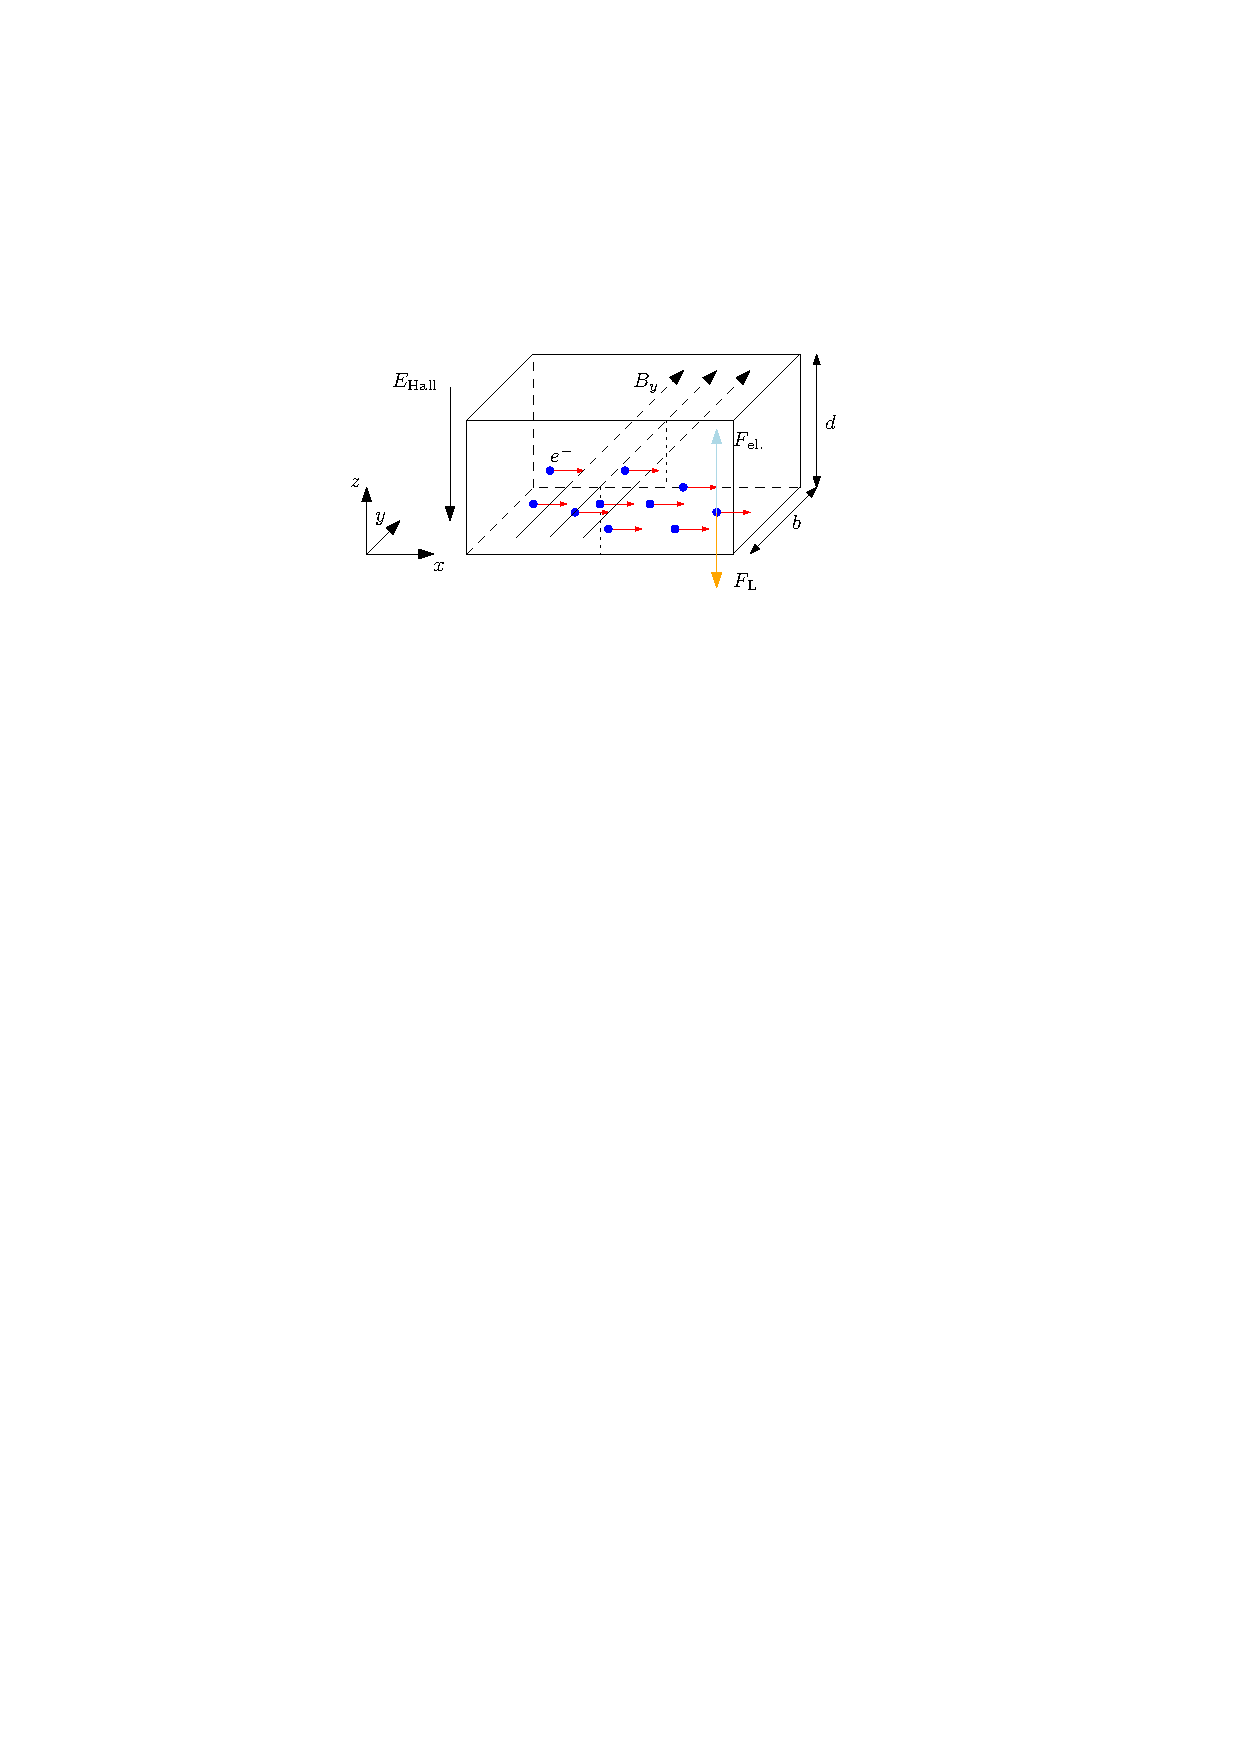
\includegraphics[width=0.65\textwidth]{./figures/hall_effekt.pdf}
	\caption{Zur Herleitung des Hall-Effekts}
	\label{fig:hall_effekt}
\end{figure}
Die Ladungsträger werden durch die Lorentzkraft soweit ausgelenkt, bis das durch die Auslenkung entstandene elektrische Feld $E_\mathrm{Hall}$ die Lorentzkraft kompensiert:
\begin{align*}
	e E_\mathrm{Hall} = e v_x B_y
	\label{eq:kompensation}
\end{align*}
Dabei ist die an den Stirnflächen mit Abstand $d$ anliegende Spannung gegeben durch $E_\mathrm{Hall} = U_\mathrm{Hall} / d$, womit aus Gleichung \ref{eq:kompensation} folgt:
\begin{align*}
	U_\mathrm{Hall} = d v_x B_y
\end{align*}
Die Geschwindigkeit der Ladungsträger $v_x$ lässt sich nun über die Stromdichte $j_x = e n v_x = I/A$ ausdrücken, wobei $A = d \cdot b$ die Querschnittsfläche des Leiters ist.
Damit folgt die Hall-Spannung:
\begin{align*}
	U_\mathrm{Hall} = \frac{I B_y}{b\, n\, e}
\end{align*}
Somit ist die Hall-Spannung proportional zum Magnetfeld $B_y$ und kann damit zur Messung desselben verwendet werden.
In der Praxis werden, um bei einem kleinen Strom $I$ eine große Spannung zu messen, häufig Halbleitermaterialien verwendet, da diese eine kleine Ladungsträgerdichte $n$ aufweisen.


\subsection{Franck-Hertz-Versuch}

Der Franck-Hertz-Versuch wurde um 1914 von James Franck und Gustav Hertz \cite{demtroeder3} durchgeführt und demonstrierte die Wichtigkeit der Energiequantelung bei Stoßprozessen.
In dem Versuch wird eine mit Quecksilber bei Unterdruck (ca. \SI{e-2}{\milli\bar}, Quecksilber im Zwei-Phasen-System gasförmig $\rightleftarrows$ flüssig) gefüllte Elektronenröhre genutzt, bei der zwischen Kathode und Anode ein Gitter eingebaut ist, und die variable Beschleunigungsspannung $U$ zwischen Kathode und Gitter anliegt.
Der Aufbau ähnelt stark einem gewöhnlichen \textbf{Triodensystem}, wobei hier die Strecke Kathode-Gitter als Beschleunigungsstrecke genutzt wird und zwischen Gitter und Anode eine Gegenspannung $\Delta U$ angelegt wird.
\begin{figure}[h]
\centering
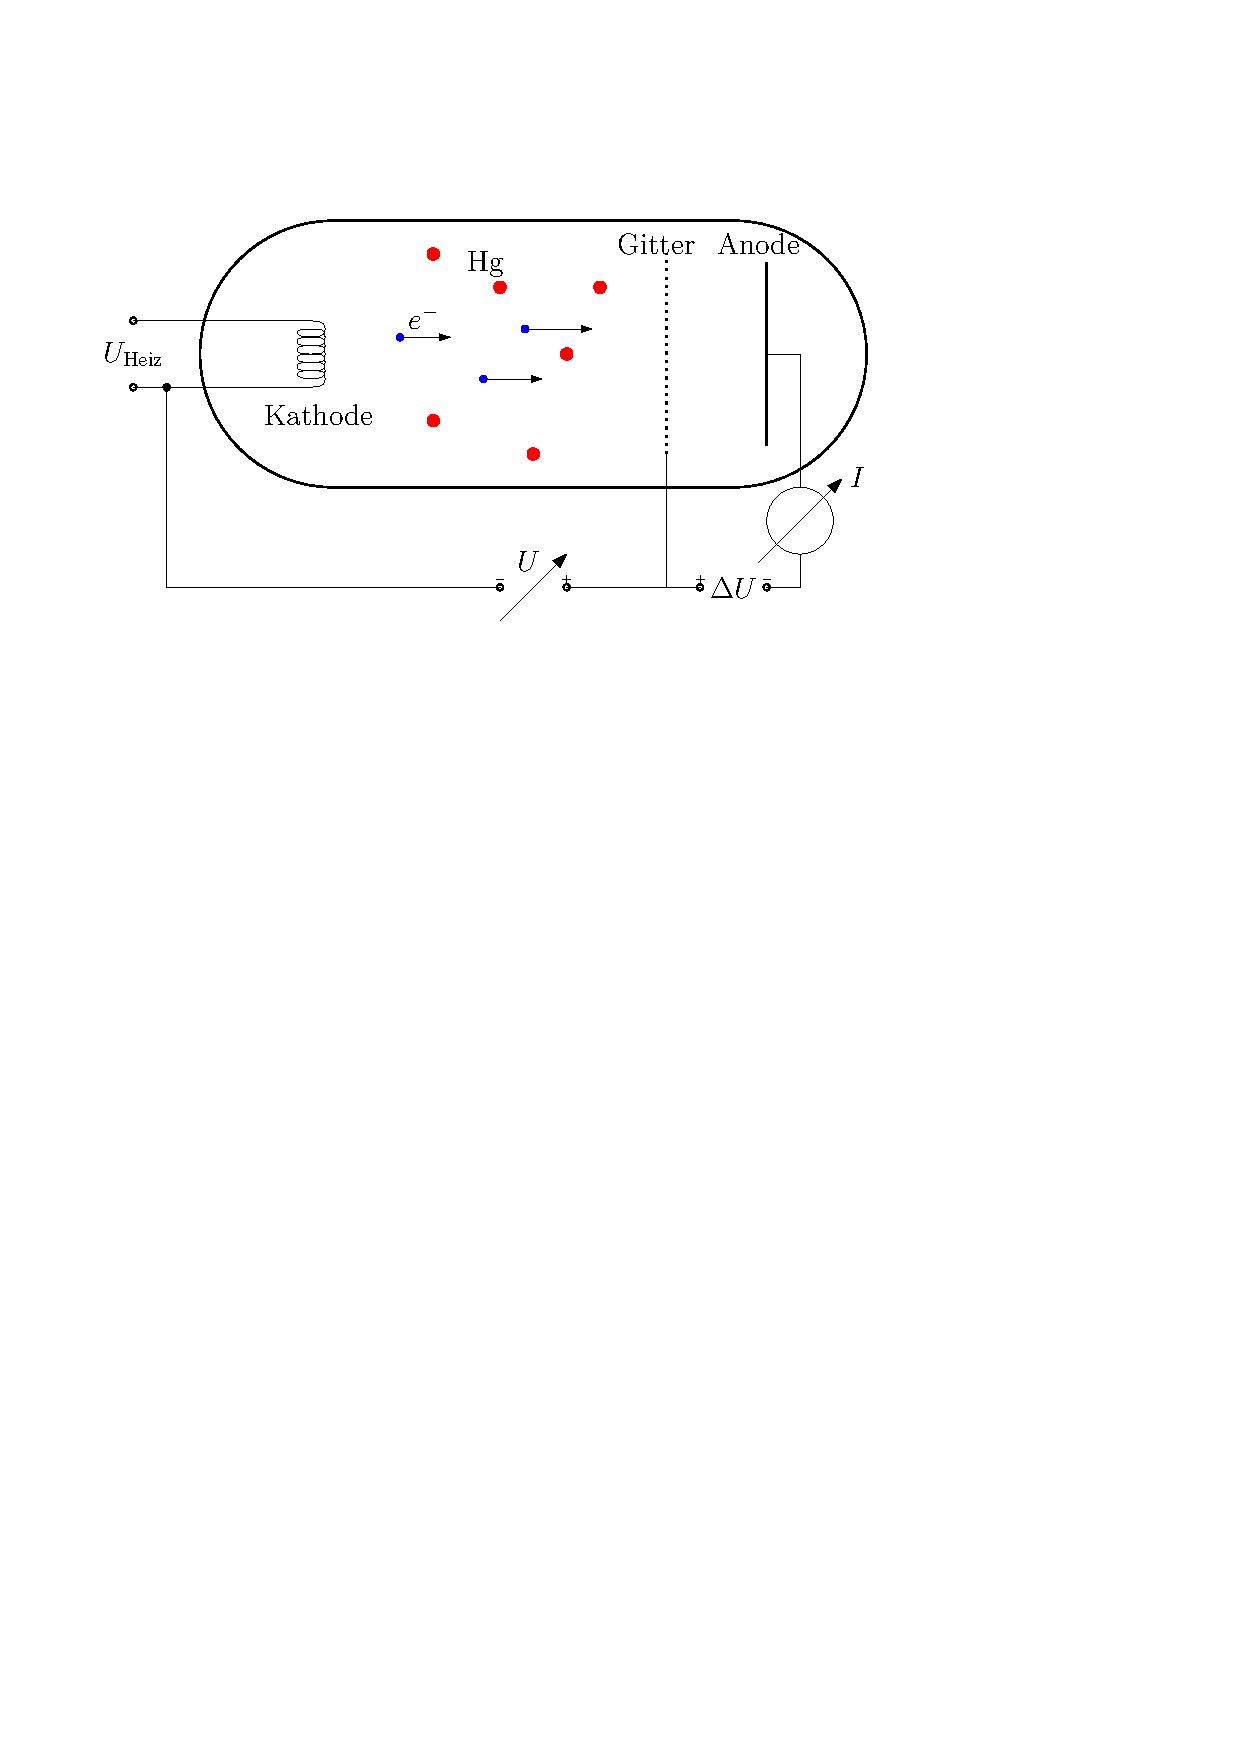
\includegraphics[width=0.7\textwidth]{./figures/franck-hertz_aufbau.pdf}
\caption{Aufbau des Franck-Hertz-Versuches}
\label{fig:franck-hertz_aufbau}
\end{figure}
Die durch den glühelektrischen Effekt (Erklärung s. \ref{sec:roehrenelektronik}) ausgetretenen Elektronen werden von dem äußeren anliegenden Feld durch die Beschleunigungsspannung zum Gitter hin beschleunigt und erreichen dabei die Energie $eU$.
Durch die zwischen Gitter und Anode anliegende Gegenspannung werden die Elektronen nach Passieren des Gitters abgebremst und nur solche mit Energien größer als $e\Delta U$ erreichen die Anode.
Dieses Messverfahren wird als \textbf{Gegenfeldmethode} bezeichnet.
\begin{figure}[h]
\centering
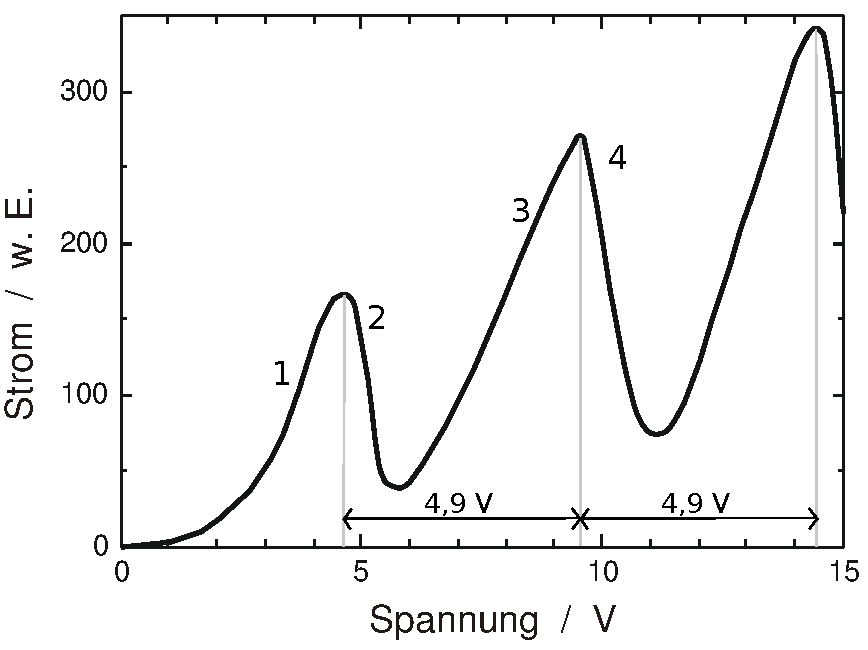
\includegraphics[width=0.5\textwidth]{./figures/franck-hertz_ergebnis.pdf}
\caption{Anodenstrom beim Franck-Hertz-Versuch mit Quecksilber, aufgetragen gegen die Beschleunigungsspannung; nach Originaldaten von Franck und Hertz. Quelle: \url{http://upload.wikimedia.org/wikipedia/commons/5/50/Franck-Hertz_de.svg} (abgerufen am 14.11.2014)}
\label{fig:franck-hertz_ergebnis}
\end{figure}
Bei der Durchführung des Versuches stellte man fest, dass der Anodenstrom sich wie in Abbildung \ref{fig:franck-hertz_ergebnis} verhält.
Man sieht dabei, dass in Abständen von \SI{4.9}{\volt} (der Wert gilt nur für Quecksilber) der Strom stark einbricht.
Der Grund dafür ist, dass die Elektronen auf der Beschleunigungsstrecke inelastische Stöße mit den Quecksilberatomen ausführen und diese dadurch anregen.
Die dabei an das Quecksilber abgegebene Energie steht den Elektronen nicht mehr zur Verfügung, um die Anode zu erreichen, der Strom bricht ein. 
Der Abstand der Maxima entspricht dabei genau der Anregungsenergie der Quecksilberatome, die in diesem Versuch bestimmt werden soll.

\subsubsection{Röhrenelektronik}
\label{sec:roehrenelektronik}
Wir nutzen zur Erzeugung der Elektronen in der Röhre den glühlektrischen Effekt durch den an der Kathode bei Anlegen einer hohen Spannung Elektronen austreten.
Dies geschieht dadurch, dass die Elektronen im Draht durch die hohe Spannung angeregt werden und die (vom Material abhängige) Austrittsarbeit überwinden.
Die Stromdichte der aus einem Metall austretenden Elektronen wird beschrieben durch die \textbf{Richardson-Gleichung} \cite{np_richardson}:
\begin{align*}
j=A\,T^2\cdot\exp\left({-\dfrac{\phi}{\mathrm{k_B}T}}\right)
\end{align*}
Dabei ist $T$ die absolute Temperatur, $\mathrm{k_B}$ die Boltzmann-Konstante und $A$ und $\phi$ (Austrittsarbeit) materialabhängige Konstanten.

Die Erzeugung von Elektronen ist dabei jedoch nicht unbegrenzt möglich.
Bei vielen austretenden Elektronen kann es passieren, dass diese durch die Beschleunigungsspannung bewegten Ladungsträger selber ein elektrisches Feld erzeugen, was dafür sorgt, dass die Elektronen, die an der Kathode entstehen, das äußere Beschleunigungsfeld nicht wahrnehmen und diese \textbf{Raumladung} um die Kathode den gemessenen Anodenstrom limitiert.
Für diesen gilt\footnote{Quelle: Vorlesung Accelerator Physics (WS 2014/2015) bei PD Dr. Hillert}:
\begin{align}
I_0=P\,U_0^{\,\frac{3}{2}}
\end{align}
mit der \emph{Perveanz} bzw. Raumladungskonstante $P$, die die Fläche der Kathode, den Abstand Kathode-Anode und die Bauart berücksichtigt.

\subsubsection{Thermodynamik und Stoßprozesse}

Zur Beschreibung des Gases in der Röhre verwenden wir in dem Versuch die kinetische Gastheorie.
Das Gas wird dabei als Menge von gleichen Teilchen vernachlässigbarer Größe aufgefasst, die sich zwischen den Stößen mit anderen Teilchen oder der Gefäßwand gleichförmig bewegen.
Außer bei den Stößen, die grundsätzlich elastisch stattfinden, wirken zwischen den Teilchen keine Kräfte.
Wir können darauf aufbauend Eigenschaften definieren wie die \textbf{mittlere freie Weglänge}, die die durchschnittliche Strecke angibt, die ein Teilchen zurücklegt, ohne Stöße mit anderen Teilchen auszuführen.
Sie ist definiert als
\begin{align}
\lambda=\frac{1}{n\sigma}
\end{align}
mit $n$ der Teilchendichte und $\sigma$ dem totalen \textbf{Wirkungsquerschnitt}.
Dieser ist ebenfalls eine wichtige Eigenschaft des Gases, denn er gibt die Wahrscheinlichkeit an, dass ein Teilchen mit einem anderen wechselwirkt, wobei wir die Wechselwirkung in der kinetischen Gastheorie wie angesprochen auf elastische Stöße beschränken.

\subsubsection{Quecksilberatom: LS- und jj-Kopplung}
Zur Erklärung des Franck-Hertz-Versuches müssen wir die Kopplung mehrerer Drehimpulskomponenten beachten.
Grundsätzlich können in Systemen mit mehreren Drehimpulskomponenten diese untereinander koppeln, wobei wir uns hier auf den Bahndrehimpuls $\ell$ und den Elektronenspin $s$ mit Quantenzahl $\pm1/2$, der als Eigendrehimpuls interpretiert werden kann, beschränken.
Der Hamiltonoperator für die Kopplung dieser beiden Drehimpulse ist gegeben durch
\begin{align*}
\hat{H}=\frac{a}{\hbar^2}\hat{\vec{\ell}}\cdot\hat{\vec{s}}\qquad a=\frac{Ze^2\mu_0\hbar^2}{8\pi m_e^2 r^3}
\end{align*}
mit der Kopplungskonstanten $a$, die von der Kernladungszahl $Z$ abhängt.
Diese Abhängigkeit von $Z$ sorgt dafür, dass die Kopplung von Spin und Bahndrehimpuls für unterschiedliche $Z$ betrachtet werden muss.
Für kleine Kernladungszahlen ist die Kopplungsenergie zwischen Elektronenspin und Bahndrehimpuls gering und kleiner als die Kopplung zwischen zwei Drehimpulsen $\ell_i$ und $\ell_j$ sowie zwischen zwei Spins $s_i$ und $s_j$, weswegen eher die Bahndrehimpulse bzw. die Spins untereinander koppeln werden.
Dann spricht man von \textbf{LS-Kopplung}.
Im Vektormodell lässt sich somit schreiben:
\begin{align*}
\vec{J}=\vec{L}+\vec{S}=\sum_i\vec{\ell}_i+\sum_i\vec{s}_i
\end{align*}
Für große $Z$ ist die Kopplung zwischen $\ell$ und $s$ größer als die Kopplung zweier Bahndrehimpulse bzw. Spins untereinander und es werden eher $\ell$ und $s$ eines Elektrons zu $j=\ell+s$ koppeln.
Die $j_i$ der Elektronen koppeln untereinander zum Gesamtdrehimpuls, so dass man im Vektormodell für die \textbf{jj-Kopplung} erhält:
\begin{align*}
\vec{J}=\sum_i\vec{j}_i=\sum_i\left(\vec{\ell}_i+\vec{s}_i\right)
\end{align*}
Dadurch ergeben sich neue \textbf{Auswahlregeln}, die die in \ref{sec:auswahlregeln} genannten (dort wurde nur LS-Kopplung berücksichtigt) vor allem um $\Delta S=\pm1$ erweitern, wodurch Übergänge zwischen verschiedenen Multiplettsystemen möglich werden, wie man im in Abbildung \ref{fig:termschema_hg} dargestellten Termschema von Quecksilber sehen kann.
\begin{figure}[!h]
\centering
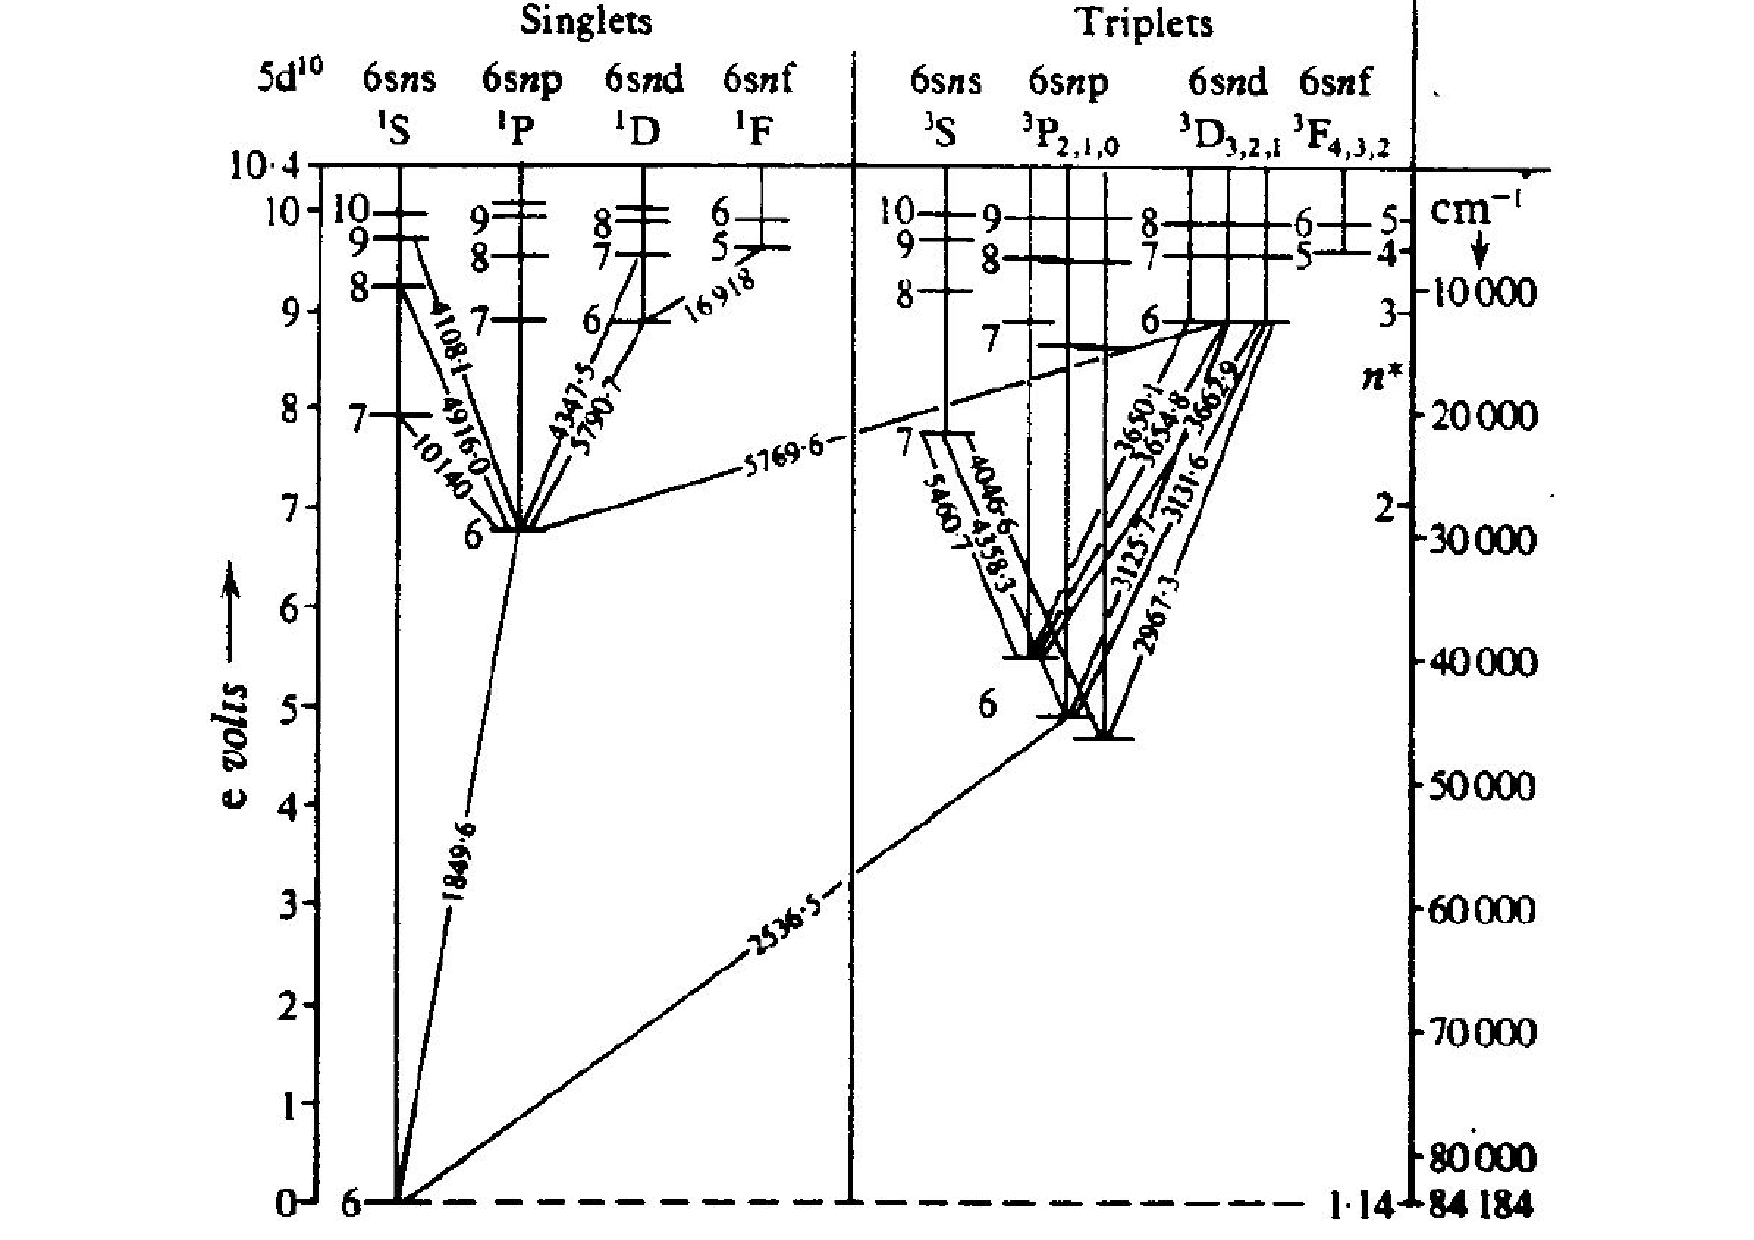
\includegraphics[width=0.9\textwidth]{./figures/termschema_hg.pdf}
\caption{Vereinfachtes Termschema von Quecksilber. Quelle: Kuhn, Atomic Spectra, S. 192, 1962}
\label{fig:termschema_hg}
\end{figure}

\clearpage

\section{Zeeman-Effekt}
In diesem Versuchsteil soll die Energieaufspaltung der $\SI{643,8470}{\nano\metre}$-Linie von Cadmium im externen Magnetfeld untersucht werden.

\subsection{Versuchsdurchführung}

\subsubsection{Versuchsaufbau und Justage}
\begin{figure}[h]
	\centering
	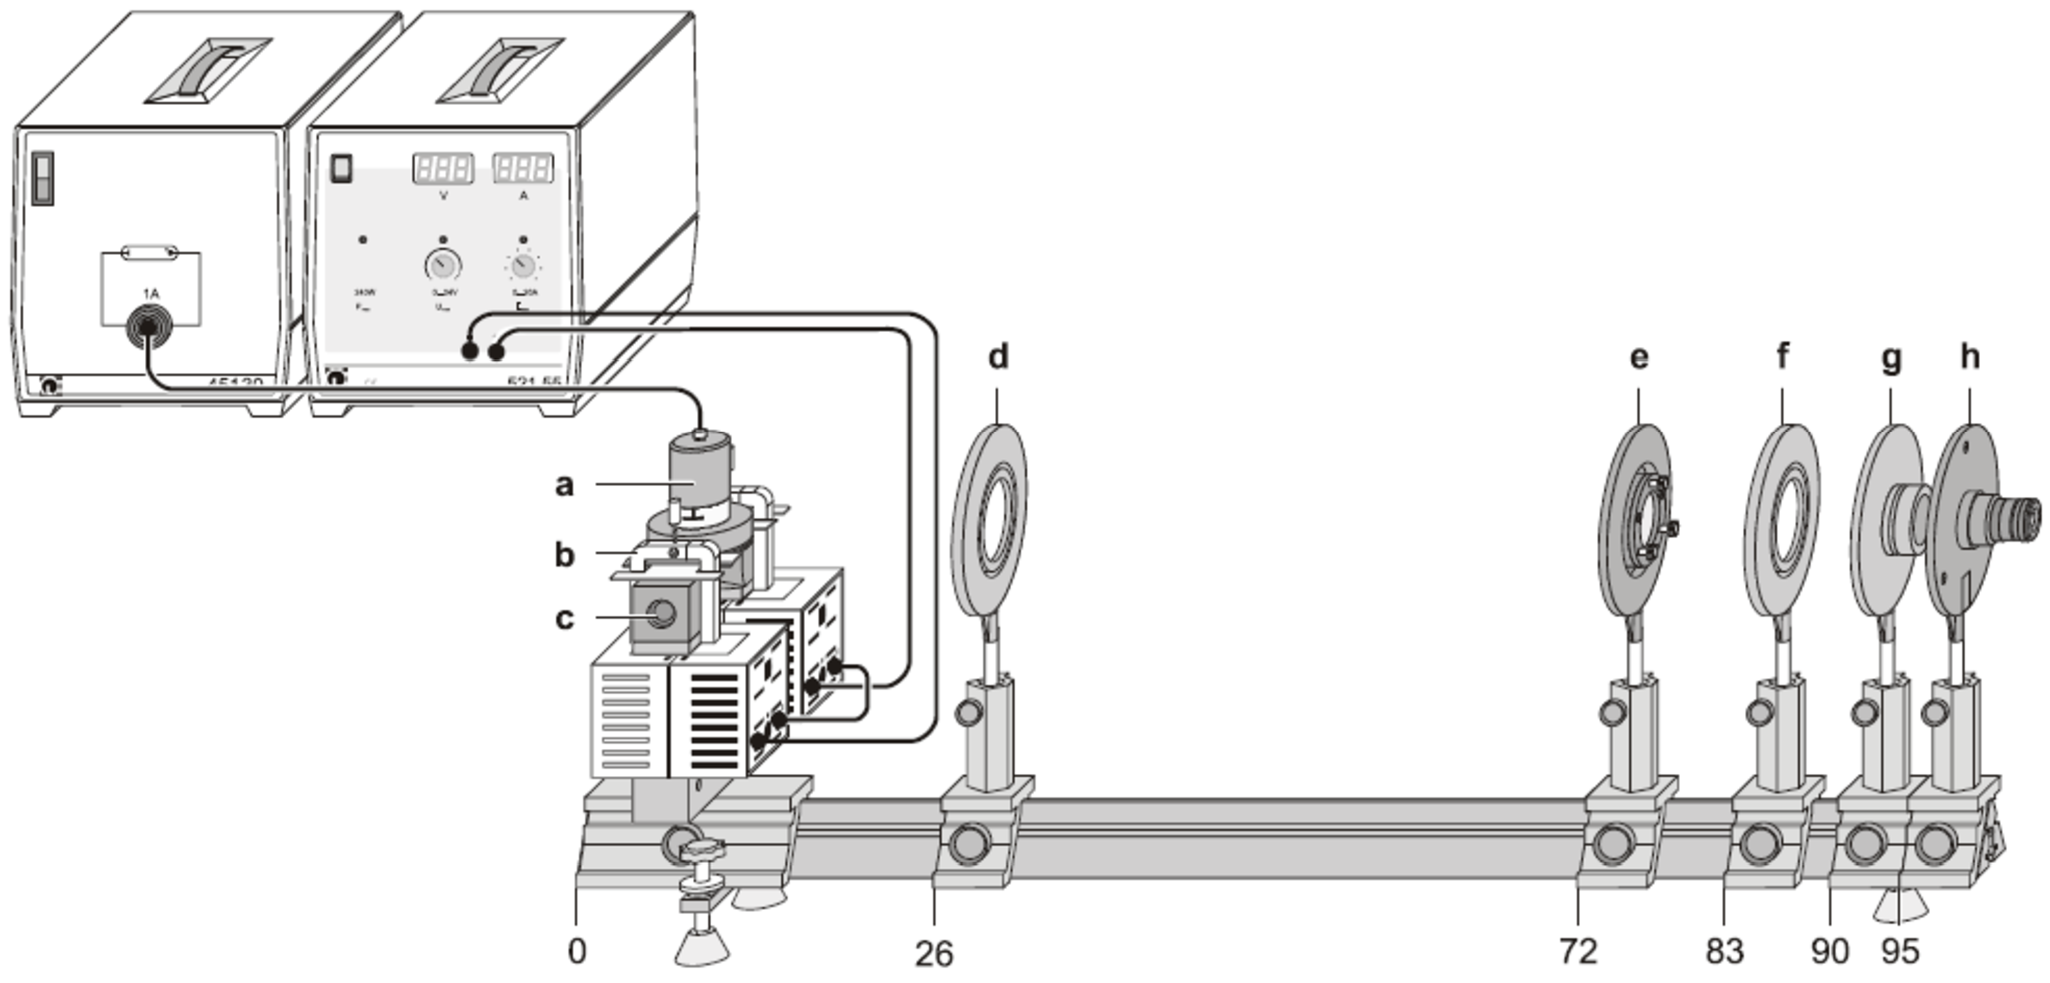
\includegraphics[width=1.0\textwidth]{./figures/aufbau_zeeman.pdf}
	\caption{transversaler Aufbau zur Beobachtung des Zeeman-Effekts. \textbf{a}) Cadmiumlampe \textbf{b}) Klammern \textbf{c}) Polschuhe \textbf{d}) Kondensorlinse $f=\SI{150}{\milli\metre}$ \textbf{e}) Fabry-Pérot-Etalon \textbf{f}) Abbildungslinse $f=\SI{150}{\milli\metre}$ \textbf{g}) Interferenzfilter \textbf{h}) Okular. Quelle: LD Didactic}
	\label{fig:aufbau_zeeman}
\end{figure}

Zur Beobachtung der Energieaufspaltung des Zeeman-Effekts bauen wir die Apparatur wie in Abbildung \ref{fig:aufbau_zeeman} auf.
Dazu führen wir zunächst die Cadmium-Lampe zwischen die Polschuhe, welche mit dem Kern der beiden Magnetspulen verbunden ist.
Dabei achten wir darauf, dass die Verbindung der Lampe mit dem Netzgerät, sowie die Abschmelzstelle des Lampenkolbens nicht im Strahlengang liegt.
Nun bauen wir die optischen Elemente (\textbf{d} -- \textbf{h}) ein.
Zur Justage der Apperatur halten wir vor das Fabry-Pérot-Etalon ein Blatt Papier und stellen die Kondensorlinse so ein, dass das Etalon komplett ausgeleuchtet wird.
Direkt vor das Okular mit scharf gestellter Strichskala stellen wir den Interferenzfilter mit Mittelwellenlänge $\lambda = \SI{643,8 +- 2}{\nano\metre}$ um das sichtbare Raumlicht zu minimieren.
Anschließend stellen wir die Abbildungslinse (\textbf{f}) so ein, dass das Etalon scharf durch das Okular abgebildet wird.
Da das Zentrum des Ringsystems nicht mit der Strichskala des Okulars übereinstimmt, kippen wir das Fabry-Pérot-Etalon mit den daran angebrachten Stellschrauben bis dies der Fall ist.

\subsubsection{Beobachtung der Aufspaltung}
Als erstes beobachten wir die Aufspaltung der Linie in \textbf{transversalem Aufbau} - das heißt, dass das Magnetfeld senkrecht zur Beobachtungsrichtung steht.
Zunächst beobachten wir das Interferenzmuster des Fabry-Pérot-Etalons, welches aus konzentrischen Kreisen besteht, die dadurch entstehen, dass das Etalon mit einer ausgedehnten Lichtquelle beleuchtet wird.
Um eine Linienaufspaltung zu beobachten, lassen wir nun mithilfe des Netzgeräts einen Strom $I$ durch die Spulen fließen.
Dadurch entsteht im Bereich des Lampenkolbens ein näherungsweise homogenes Magnetfeld.
Wir wählen den Strom so, dass wir eine deutliche Aufspaltung der Kreise des Interferenzmusters erkennen können.
Um die Polarisation zu untersuchen, stellen wir einen Polarisationsfilter in den Strahlengang und skizzieren das am Okular sichtbare Interferenzmuster bei verschiedenen Filterausrichtungen.
Wir entfernen den Filter und beobachten nun die Aufspaltung der Linien im Okular während wir langsam den Spulenstrom verringern.
Dabei bestimmen wir den Spulenstrom, bei dem die Aufspaltung der Ringe gerade noch zu erkennen ist.
Diese Messung führen wir insgesamt fünf mal durch, um den Messfehler besser abschätzen zu können.

Nun drehen wir die Polschuhe mitsamt Spulen so, dass wir in \text{longitudinalem Aufbau} beobachten können (das Magnetfeld zeigt in Beobachtungsrichtung).
Die Cadmiumlampe beleuchtet dabei die Kondensorlinse durch ein Loch im Polschuh.
Wir beobachten ohne Magnetfeld das Interferenzmuster des transversalen Aufbaus.
Eine Messung mit zugeschaltetem Magnetfeld führt hier jedoch zur Aufspaltung in zwei konzentrische Kreise (eigentlich drei $\pi$-Linie war schwach zu sehen).
Alle Skizzen in Abbildung \ref{fig:zeeman_transversal}.
Im Gegensatz zur transversalen Beobachtung verwenden wir hier eine Kombination von Polarisationsfilter und $\frac{\lambda}{4}$-Platte zur Bestimmung der Polarisation.
Dazu stellen wir die Viertel-Wellenlängen-Platte unter festem Winkel $\SI{0}{\degree}$ vor den Polarisationsfilter (in Strahlrichtung), dessen Ausrichtung $\alpha$ wir variieren und skizzieren das sichtbare Interferenzbild.
Wie bei der transversalen Beobachtung bestimmen wir auch hier, nach dem Entfernen von Filter und $\frac{\lambda}{4}$-Platte, den minimalen Strom, bei dem die Aufspaltung gerade noch erkannt werden kann.
Alle Skizzen in Abbildung \ref{fig:zeeman_longitudinal}.

\subsubsection{Messung des Zeeman-Effekts}

\begin{figure}[h]
\centering
% GNUPLOT: LaTeX picture with Postscript
\begingroup
  \makeatletter
  \providecommand\color[2][]{%
    \GenericError{(gnuplot) \space\space\space\@spaces}{%
      Package color not loaded in conjunction with
      terminal option `colourtext'%
    }{See the gnuplot documentation for explanation.%
    }{Either use 'blacktext' in gnuplot or load the package
      color.sty in LaTeX.}%
    \renewcommand\color[2][]{}%
  }%
  \providecommand\includegraphics[2][]{%
    \GenericError{(gnuplot) \space\space\space\@spaces}{%
      Package graphicx or graphics not loaded%
    }{See the gnuplot documentation for explanation.%
    }{The gnuplot epslatex terminal needs graphicx.sty or graphics.sty.}%
    \renewcommand\includegraphics[2][]{}%
  }%
  \providecommand\rotatebox[2]{#2}%
  \@ifundefined{ifGPcolor}{%
    \newif\ifGPcolor
    \GPcolortrue
  }{}%
  \@ifundefined{ifGPblacktext}{%
    \newif\ifGPblacktext
    \GPblacktexttrue
  }{}%
  % define a \g@addto@macro without @ in the name:
  \let\gplgaddtomacro\g@addto@macro
  % define empty templates for all commands taking text:
  \gdef\gplbacktext{}%
  \gdef\gplfronttext{}%
  \makeatother
  \ifGPblacktext
    % no textcolor at all
    \def\colorrgb#1{}%
    \def\colorgray#1{}%
  \else
    % gray or color?
    \ifGPcolor
      \def\colorrgb#1{\color[rgb]{#1}}%
      \def\colorgray#1{\color[gray]{#1}}%
      \expandafter\def\csname LTw\endcsname{\color{white}}%
      \expandafter\def\csname LTb\endcsname{\color{black}}%
      \expandafter\def\csname LTa\endcsname{\color{black}}%
      \expandafter\def\csname LT0\endcsname{\color[rgb]{1,0,0}}%
      \expandafter\def\csname LT1\endcsname{\color[rgb]{0,1,0}}%
      \expandafter\def\csname LT2\endcsname{\color[rgb]{0,0,1}}%
      \expandafter\def\csname LT3\endcsname{\color[rgb]{1,0,1}}%
      \expandafter\def\csname LT4\endcsname{\color[rgb]{0,1,1}}%
      \expandafter\def\csname LT5\endcsname{\color[rgb]{1,1,0}}%
      \expandafter\def\csname LT6\endcsname{\color[rgb]{0,0,0}}%
      \expandafter\def\csname LT7\endcsname{\color[rgb]{1,0.3,0}}%
      \expandafter\def\csname LT8\endcsname{\color[rgb]{0.5,0.5,0.5}}%
    \else
      % gray
      \def\colorrgb#1{\color{black}}%
      \def\colorgray#1{\color[gray]{#1}}%
      \expandafter\def\csname LTw\endcsname{\color{white}}%
      \expandafter\def\csname LTb\endcsname{\color{black}}%
      \expandafter\def\csname LTa\endcsname{\color{black}}%
      \expandafter\def\csname LT0\endcsname{\color{black}}%
      \expandafter\def\csname LT1\endcsname{\color{black}}%
      \expandafter\def\csname LT2\endcsname{\color{black}}%
      \expandafter\def\csname LT3\endcsname{\color{black}}%
      \expandafter\def\csname LT4\endcsname{\color{black}}%
      \expandafter\def\csname LT5\endcsname{\color{black}}%
      \expandafter\def\csname LT6\endcsname{\color{black}}%
      \expandafter\def\csname LT7\endcsname{\color{black}}%
      \expandafter\def\csname LT8\endcsname{\color{black}}%
    \fi
  \fi
  \setlength{\unitlength}{0.0500bp}%
  \begin{picture}(7200.00,5760.00)%
    \gplgaddtomacro\gplbacktext{%
      \csname LTb\endcsname%
      \put(946,704){\makebox(0,0)[r]{\strut{} 0}}%
      \csname LTb\endcsname%
      \put(946,1388){\makebox(0,0)[r]{\strut{} 100}}%
      \csname LTb\endcsname%
      \put(946,2073){\makebox(0,0)[r]{\strut{} 200}}%
      \csname LTb\endcsname%
      \put(946,2757){\makebox(0,0)[r]{\strut{} 300}}%
      \csname LTb\endcsname%
      \put(946,3442){\makebox(0,0)[r]{\strut{} 400}}%
      \csname LTb\endcsname%
      \put(946,4126){\makebox(0,0)[r]{\strut{} 500}}%
      \csname LTb\endcsname%
      \put(946,4811){\makebox(0,0)[r]{\strut{} 600}}%
      \csname LTb\endcsname%
      \put(946,5495){\makebox(0,0)[r]{\strut{} 700}}%
      \csname LTb\endcsname%
      \put(1078,484){\makebox(0,0){\strut{} 0}}%
      \csname LTb\endcsname%
      \put(1651,484){\makebox(0,0){\strut{} 1}}%
      \csname LTb\endcsname%
      \put(2223,484){\makebox(0,0){\strut{} 2}}%
      \csname LTb\endcsname%
      \put(2796,484){\makebox(0,0){\strut{} 3}}%
      \csname LTb\endcsname%
      \put(3368,484){\makebox(0,0){\strut{} 4}}%
      \csname LTb\endcsname%
      \put(3941,484){\makebox(0,0){\strut{} 5}}%
      \csname LTb\endcsname%
      \put(4513,484){\makebox(0,0){\strut{} 6}}%
      \csname LTb\endcsname%
      \put(5086,484){\makebox(0,0){\strut{} 7}}%
      \csname LTb\endcsname%
      \put(5658,484){\makebox(0,0){\strut{} 8}}%
      \csname LTb\endcsname%
      \put(6231,484){\makebox(0,0){\strut{} 9}}%
      \csname LTb\endcsname%
      \put(6803,484){\makebox(0,0){\strut{} 10}}%
      \put(176,3099){\rotatebox{-270}{\makebox(0,0){\strut{}Magnetfeld $B$ im Luftspalt / \si{\milli\tesla}}}}%
      \put(3940,154){\makebox(0,0){\strut{}Spulenstrom $I$ / \si{\ampere}}}%
      \put(3940,5385){\makebox(0,0){\strut{}}}%
    }%
    \gplgaddtomacro\gplfronttext{%
      \csname LTb\endcsname%
      \put(2662,5322){\makebox(0,0)[r]{\strut{}Messwerte}}%
      \csname LTb\endcsname%
      \put(2662,5102){\makebox(0,0)[r]{\strut{}Fitfunktion}}%
    }%
    \gplbacktext
    \put(0,0){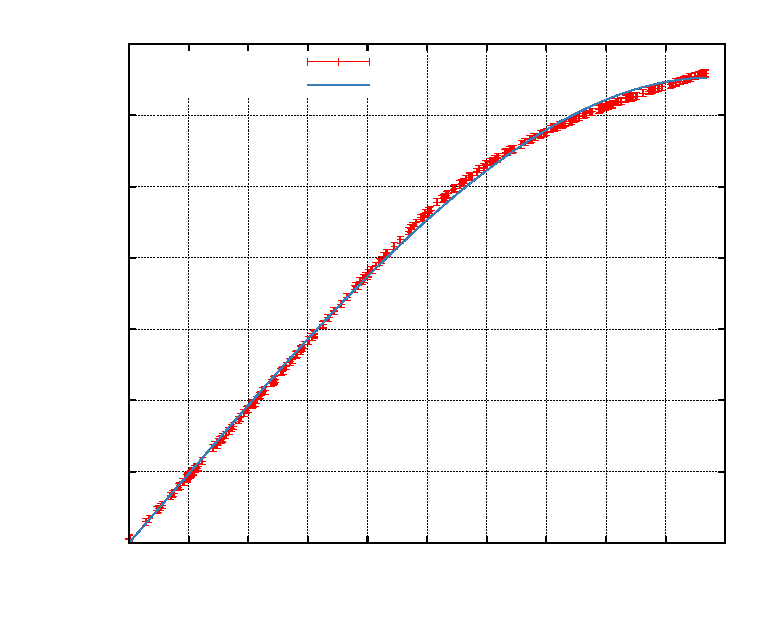
\includegraphics{./plots/kalibrierung1}}%
    \gplfronttext
  \end{picture}%
\endgroup

\caption{Erste Magnetfeldkalibrierung mit angepasstem Polynom 3. Grades ($\chi_\mathrm{d.o.f.}^2=1,48$)}
\label{fig:kalibrierung1}
\end{figure}
\begin{figure}[h]
\centering
% GNUPLOT: LaTeX picture with Postscript
\begingroup
  \makeatletter
  \providecommand\color[2][]{%
    \GenericError{(gnuplot) \space\space\space\@spaces}{%
      Package color not loaded in conjunction with
      terminal option `colourtext'%
    }{See the gnuplot documentation for explanation.%
    }{Either use 'blacktext' in gnuplot or load the package
      color.sty in LaTeX.}%
    \renewcommand\color[2][]{}%
  }%
  \providecommand\includegraphics[2][]{%
    \GenericError{(gnuplot) \space\space\space\@spaces}{%
      Package graphicx or graphics not loaded%
    }{See the gnuplot documentation for explanation.%
    }{The gnuplot epslatex terminal needs graphicx.sty or graphics.sty.}%
    \renewcommand\includegraphics[2][]{}%
  }%
  \providecommand\rotatebox[2]{#2}%
  \@ifundefined{ifGPcolor}{%
    \newif\ifGPcolor
    \GPcolortrue
  }{}%
  \@ifundefined{ifGPblacktext}{%
    \newif\ifGPblacktext
    \GPblacktexttrue
  }{}%
  % define a \g@addto@macro without @ in the name:
  \let\gplgaddtomacro\g@addto@macro
  % define empty templates for all commands taking text:
  \gdef\gplbacktext{}%
  \gdef\gplfronttext{}%
  \makeatother
  \ifGPblacktext
    % no textcolor at all
    \def\colorrgb#1{}%
    \def\colorgray#1{}%
  \else
    % gray or color?
    \ifGPcolor
      \def\colorrgb#1{\color[rgb]{#1}}%
      \def\colorgray#1{\color[gray]{#1}}%
      \expandafter\def\csname LTw\endcsname{\color{white}}%
      \expandafter\def\csname LTb\endcsname{\color{black}}%
      \expandafter\def\csname LTa\endcsname{\color{black}}%
      \expandafter\def\csname LT0\endcsname{\color[rgb]{1,0,0}}%
      \expandafter\def\csname LT1\endcsname{\color[rgb]{0,1,0}}%
      \expandafter\def\csname LT2\endcsname{\color[rgb]{0,0,1}}%
      \expandafter\def\csname LT3\endcsname{\color[rgb]{1,0,1}}%
      \expandafter\def\csname LT4\endcsname{\color[rgb]{0,1,1}}%
      \expandafter\def\csname LT5\endcsname{\color[rgb]{1,1,0}}%
      \expandafter\def\csname LT6\endcsname{\color[rgb]{0,0,0}}%
      \expandafter\def\csname LT7\endcsname{\color[rgb]{1,0.3,0}}%
      \expandafter\def\csname LT8\endcsname{\color[rgb]{0.5,0.5,0.5}}%
    \else
      % gray
      \def\colorrgb#1{\color{black}}%
      \def\colorgray#1{\color[gray]{#1}}%
      \expandafter\def\csname LTw\endcsname{\color{white}}%
      \expandafter\def\csname LTb\endcsname{\color{black}}%
      \expandafter\def\csname LTa\endcsname{\color{black}}%
      \expandafter\def\csname LT0\endcsname{\color{black}}%
      \expandafter\def\csname LT1\endcsname{\color{black}}%
      \expandafter\def\csname LT2\endcsname{\color{black}}%
      \expandafter\def\csname LT3\endcsname{\color{black}}%
      \expandafter\def\csname LT4\endcsname{\color{black}}%
      \expandafter\def\csname LT5\endcsname{\color{black}}%
      \expandafter\def\csname LT6\endcsname{\color{black}}%
      \expandafter\def\csname LT7\endcsname{\color{black}}%
      \expandafter\def\csname LT8\endcsname{\color{black}}%
    \fi
  \fi
  \setlength{\unitlength}{0.0500bp}%
  \begin{picture}(7200.00,5760.00)%
    \gplgaddtomacro\gplbacktext{%
      \csname LTb\endcsname%
      \put(946,704){\makebox(0,0)[r]{\strut{} 0}}%
      \csname LTb\endcsname%
      \put(946,1388){\makebox(0,0)[r]{\strut{} 100}}%
      \csname LTb\endcsname%
      \put(946,2073){\makebox(0,0)[r]{\strut{} 200}}%
      \csname LTb\endcsname%
      \put(946,2757){\makebox(0,0)[r]{\strut{} 300}}%
      \csname LTb\endcsname%
      \put(946,3442){\makebox(0,0)[r]{\strut{} 400}}%
      \csname LTb\endcsname%
      \put(946,4126){\makebox(0,0)[r]{\strut{} 500}}%
      \csname LTb\endcsname%
      \put(946,4811){\makebox(0,0)[r]{\strut{} 600}}%
      \csname LTb\endcsname%
      \put(946,5495){\makebox(0,0)[r]{\strut{} 700}}%
      \csname LTb\endcsname%
      \put(1078,484){\makebox(0,0){\strut{} 0}}%
      \csname LTb\endcsname%
      \put(1651,484){\makebox(0,0){\strut{} 1}}%
      \csname LTb\endcsname%
      \put(2223,484){\makebox(0,0){\strut{} 2}}%
      \csname LTb\endcsname%
      \put(2796,484){\makebox(0,0){\strut{} 3}}%
      \csname LTb\endcsname%
      \put(3368,484){\makebox(0,0){\strut{} 4}}%
      \csname LTb\endcsname%
      \put(3941,484){\makebox(0,0){\strut{} 5}}%
      \csname LTb\endcsname%
      \put(4513,484){\makebox(0,0){\strut{} 6}}%
      \csname LTb\endcsname%
      \put(5086,484){\makebox(0,0){\strut{} 7}}%
      \csname LTb\endcsname%
      \put(5658,484){\makebox(0,0){\strut{} 8}}%
      \csname LTb\endcsname%
      \put(6231,484){\makebox(0,0){\strut{} 9}}%
      \csname LTb\endcsname%
      \put(6803,484){\makebox(0,0){\strut{} 10}}%
      \put(176,3099){\rotatebox{-270}{\makebox(0,0){\strut{}Magnetfeld $B$ im Luftspalt / \si{\milli\tesla}}}}%
      \put(3940,154){\makebox(0,0){\strut{}Spulenstrom $I$ / \si{\ampere}}}%
      \put(3940,5385){\makebox(0,0){\strut{}}}%
    }%
    \gplgaddtomacro\gplfronttext{%
      \csname LTb\endcsname%
      \put(2662,5322){\makebox(0,0)[r]{\strut{}Messwerte}}%
      \csname LTb\endcsname%
      \put(2662,5102){\makebox(0,0)[r]{\strut{}Fitfunktion}}%
    }%
    \gplbacktext
    \put(0,0){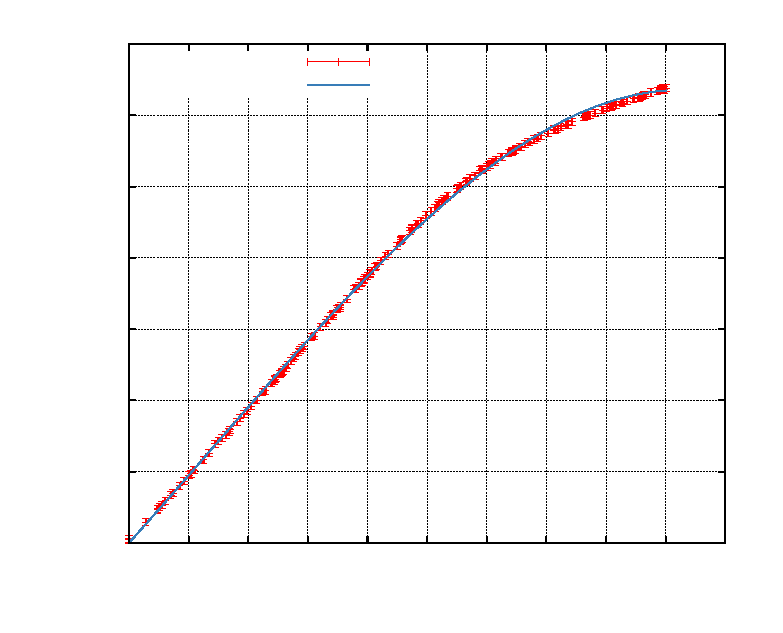
\includegraphics{./plots/kalibrierung2}}%
    \gplfronttext
  \end{picture}%
\endgroup

\caption{Zweite Magnetfeldkalibrierung mit angepasstem Polynom 3. Grades ($\chi_\mathrm{d.o.f.}^2=0,72$)}
\label{fig:kalibrierung2}
\end{figure}

\FloatBarrier

\subsection{Auswertung}

\subsubsection{Beobachtung des Zeeman-Effektes}
In der transversalen Konfiguration wird eine Aufspaltung der Ringe in drei Komponenten festgestellt.
Diese Aufspaltung entspricht allen drei möglichen Dipolübergängen $\Delta m_j = 0, \pm 1$ von $^1D_2$ nach $^1P_1$ wie in Abbildung \ref{fig:termschema_cadmium} zu sehen ist.
Dabei entsprechen die äußeren Linien den Übergängen mit $\Delta m_j = \pm 1$ und die Innere $\Delta m_j = 0$.
Um dies zu verstehen, muss die Polarisation der Linien betrachtet werden, welche wir anhand eines Polarisationsfilters analysiert haben.
In Abbildung $\ref{fig:zeeman_transversal}$ sehen wir, dass nur die mittlere Linie durch den Filter bei $\alpha_\mathrm{Pol.} = \SI{90 +- 2,5}{\degree}$ (Polarisationsebene parallel zum Magnetfeld) transmittiert wird,  das Photon ist demnach linear in der Magnetfeldrichtung polarisiert.
Im Gegensatz dazu, verschwindet die mittlere Linie bei Drehung des Filters auf $\alpha_\mathrm{Pol.} = \SI{0 +- 2,5}{\degree}$ und die beiden äußeren Linien werden transmittiert, sodass diese senkrecht auf der Magnetfeldrichtung polarisiert sind.
\begin{figure}[h]
	\centering
	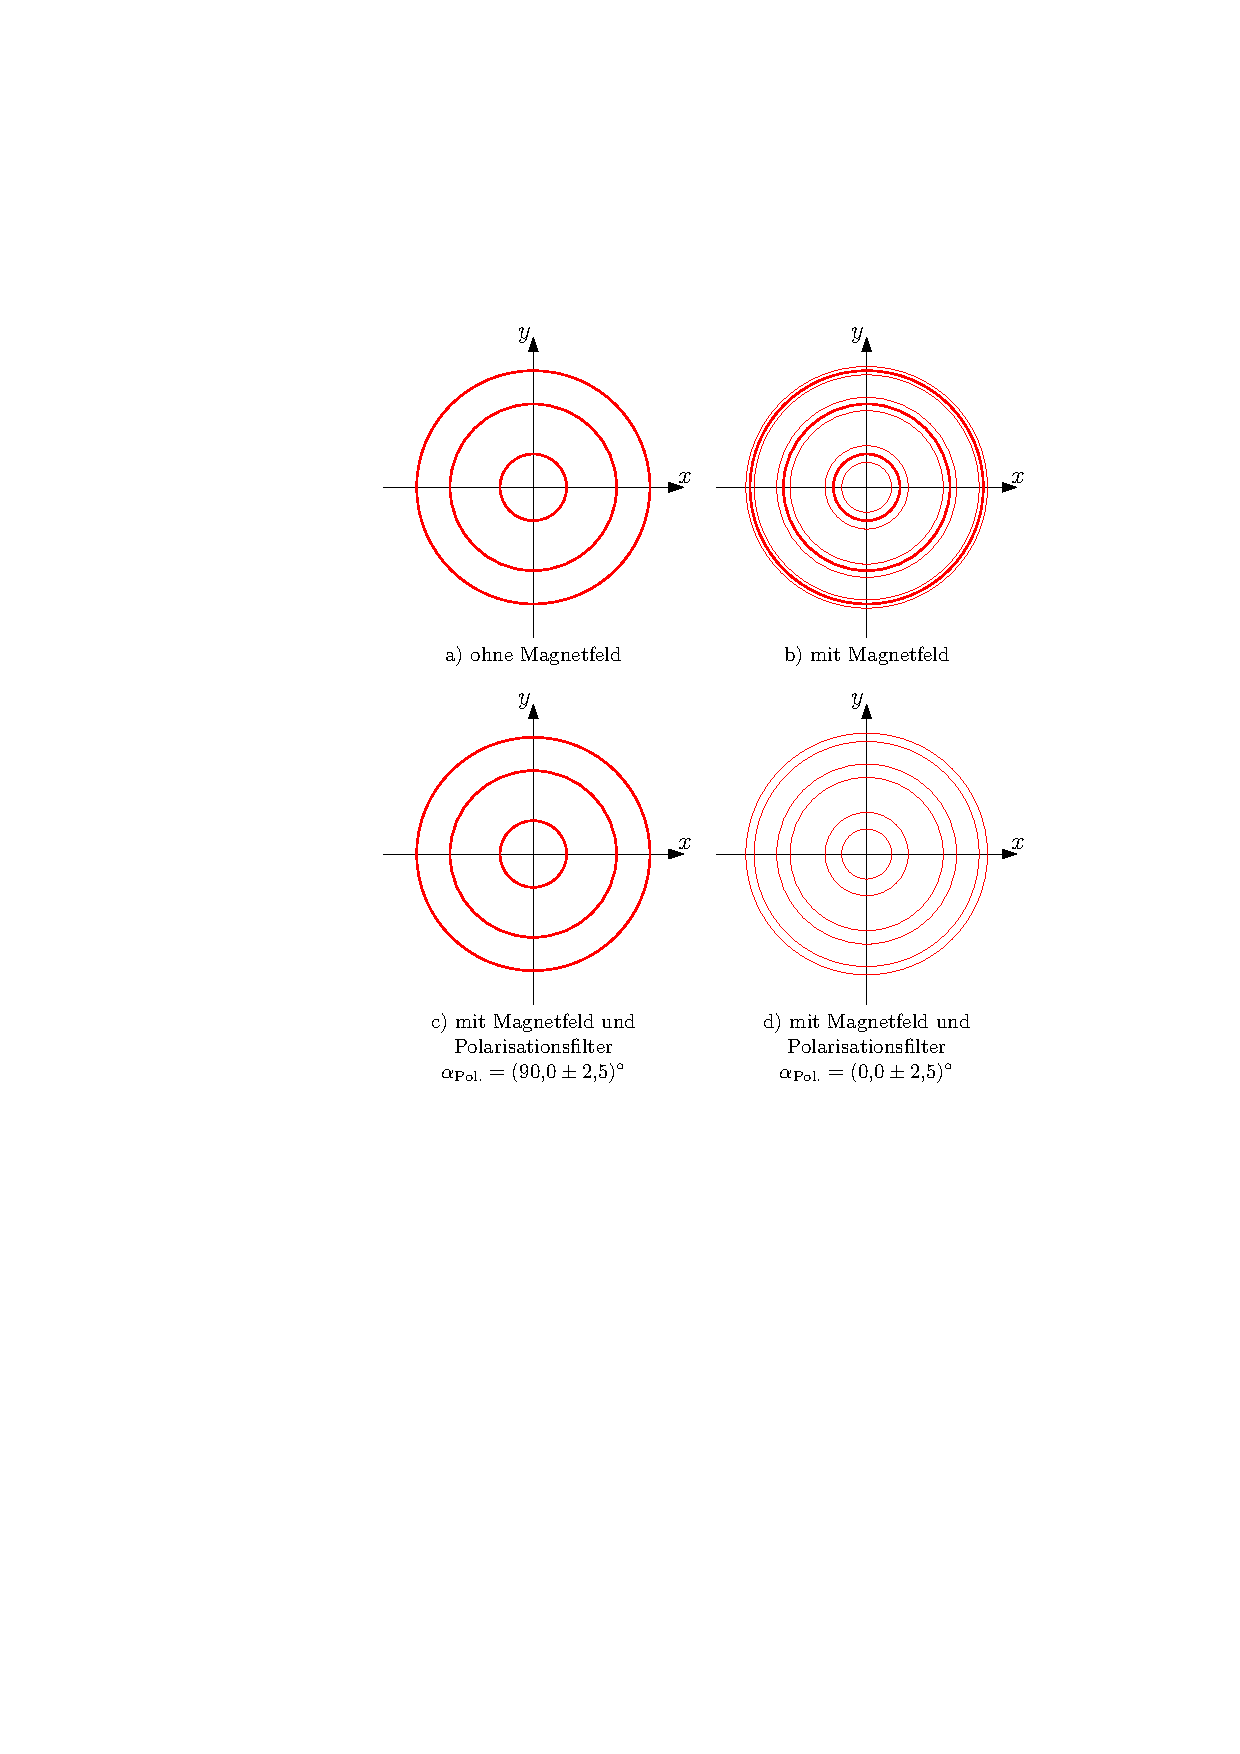
\includegraphics[width=0.8\textwidth]{./figures/zeeman_transversal.pdf}
	\caption{Interferenzmuster des Fabry-Pérot-Etalons in transversaler Konfiguration}
	\label{fig:zeeman_transversal}
\end{figure}

In der longitudinalen Konfiguration sehen wir im Wesentlichen\footnote{Die $\pi$-Linie (im Bild gepunktet) ist mit sehr geringer Intensität zu erkennen, was an Inhomogenitäten des Magnetfeldes und einer kleinen Abweichung der Beobachtungsrichtung von der Magnetfeldachse liegen kann.} eine Aufspaltung in zwei konzentrische Ringe, welche den beiden äußeren der transversalen Beobachtung entsprechen ($\Delta m = \pm 1$).
Zur Untersuchung der Polarisation nutzten wir aus, dass eine $\frac{\lambda}{4}$-Platte entgegengesetzt zirkular polarisierte Wellen in zwei senkrecht aufeinander stehende linear polarisierte Wellen zerlegt.
So kann mit einem, hinter der Viertel-Wellenlängen-Platte befindlichem, Polarisationsfilter das Licht auf zirkulare Polarisation untersucht werden.
Wir stellen fest, dass eine Einstellung des Filters auf $\alpha_\mathrm{Pol.} = \SI{-45 +- 2,5}{\degree}$ den I und $\alpha_\mathrm{Pol.} = \SI{+45 +- 2,5}{\degree}$ den äußeren Ring verschwinden lässt.
Dadurch schließen wir, dass die äußeren Ringe entgegengesetzt zirkular polarisiert sind.
\begin{figure}[h]
	\centering
	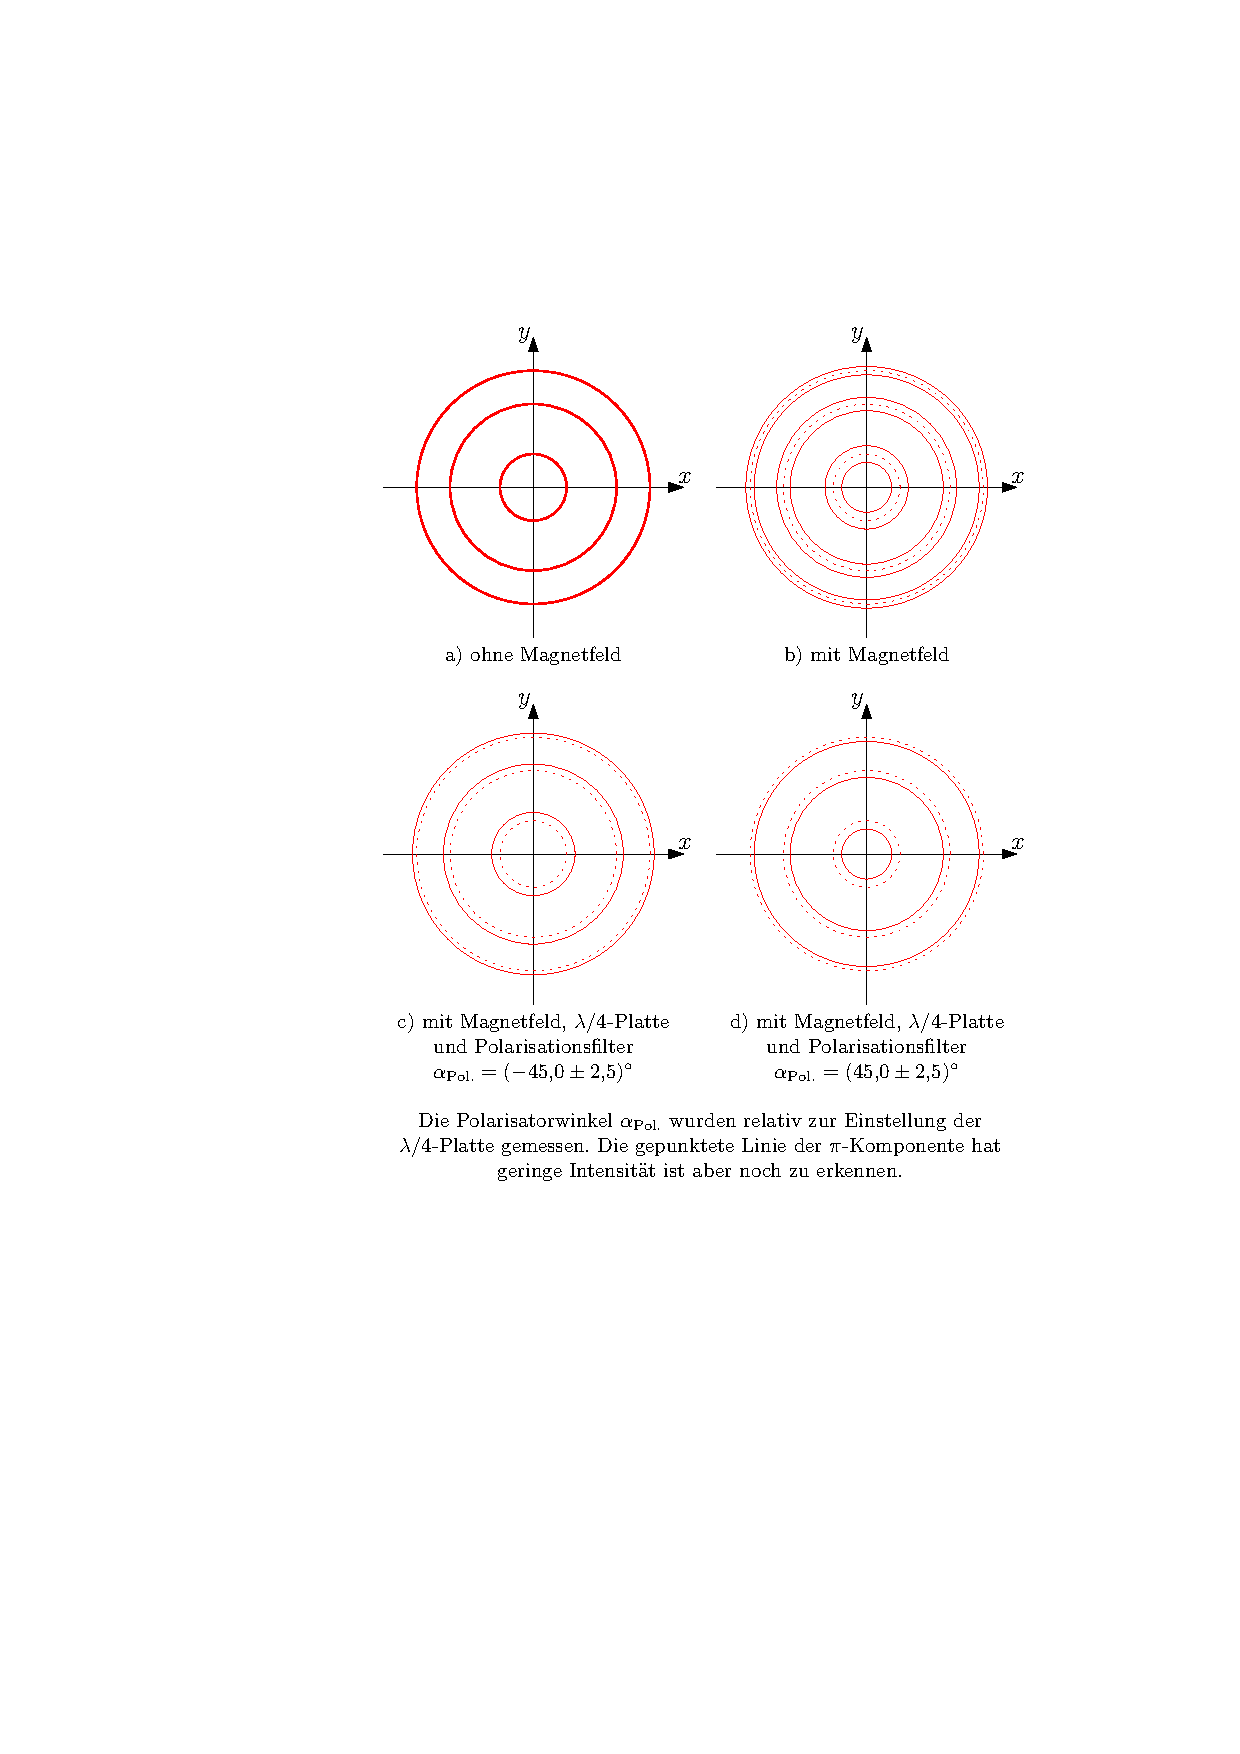
\includegraphics[width=0.8\textwidth]{./figures/zeeman_longitudinal.pdf}
	\caption{Interferenzmuster des Fabry-Pérot-Etalons in longitudinaler Konfiguration}
	\label{fig:zeeman_longitudinal}
\end{figure}

Die sichtbaren Polarisationen erklären sich wie folgt:
\begin{itemize}
	\item $\Delta m_\ell = 0$: Solche Übergänge weisen eine dipolartige Abstrahlcharakteristik in Richtung der Quantisierungsachse des Drehimpulses auf.
	Da diese Achse durch das Anlegen eines Magnetfeldes auf die Feldrichtung festgelegt ist, folgt aus der Dipolcharakteristik, dass keine Abstrahlung in Richtung der Magnetfeldachse erfolgt und somit diese Linien in longitudinaler Konfiguration nicht sichtbar sind.
	Bei jedem Dipolübergang findet eine Drehimpulsänderung $\Delta \ell = \pm 1$ statt, da das emittierte Photon ein Spin-1 Teilchen ist.
	Damit folgt aus der Drehimpulserhaltung, dass das Photon parallel zur Magnetfeldachse polarisiert sein muss, um $\Delta m_\ell = 0$ zu gewährleisten.
	
	\item $\Delta m_\ell = \pm 1$: Diese Übergänge weisen keine dipolartige Abstrahlcharakteristik auf, sodass Emission auch in Richtung des Magnetfeldes stattfindet.
	Da auch hier Drehimpulserhaltung gilt, muss der Spin des emittierten Photons so ausgerichtet sein, dass $m_s = \mp 1$ gilt, um $\Delta m = \pm 1$ zu gewährleisten.
	Diese Photonenspins entsprechen in longitudinaler Beobachtungsrichtung zirkular polarisiertem Licht und in Transversaler linear polarisiertem Licht mit Polarisationsebene senkrecht auf der Spinquantisierungsachse welche mit der Magnetfeldachse übereinstimmt.
\end{itemize}


\subsubsection{Magnetfeldkalibrierung}
Höhere Ordnungen verursachen extrem hohen Parameterfehler was dazu führt, dass der Magnetfeldfehler um eine größenordnung wächst

\begin{itemize}
	\item \textbf{Kalibration 1:}
	\begin{align}
	B_1(I) = \SI{-0.389 +- 0.014}{\milli\tesla\per\ampere\cubed} &\cdot I^3 \nonumber\\
	+\SI{0.747+-0.182}{\milli\tesla\per\ampere\squared} &\cdot I^2 \nonumber\\
	+ \SI{96.606 +- 0.602}{\milli\tesla\per\ampere} &\cdot I
	\end{align}
	\item \textbf{Kalibration 2:}
	\begin{align}
	B_2(I) = \SI{-0.518 +- 0.014}{\milli\tesla\per\ampere\cubed} &\cdot I^3 \nonumber\\
	+\SI{2.153+-0.183}{\milli\tesla\per\ampere\squared} &\cdot I^2 \nonumber\\
	+ \SI{93.086 +- 0.566}{\milli\tesla\per\ampere} &\cdot I
	\end{align}
\end{itemize}

\FloatBarrier
\subsubsection{Bestimmung des Bohrschen Magnetons}
\label{sssec:magneton}
\begin{figure}[h]
	\centering
	% GNUPLOT: LaTeX picture with Postscript
\begingroup
  \makeatletter
  \providecommand\color[2][]{%
    \GenericError{(gnuplot) \space\space\space\@spaces}{%
      Package color not loaded in conjunction with
      terminal option `colourtext'%
    }{See the gnuplot documentation for explanation.%
    }{Either use 'blacktext' in gnuplot or load the package
      color.sty in LaTeX.}%
    \renewcommand\color[2][]{}%
  }%
  \providecommand\includegraphics[2][]{%
    \GenericError{(gnuplot) \space\space\space\@spaces}{%
      Package graphicx or graphics not loaded%
    }{See the gnuplot documentation for explanation.%
    }{The gnuplot epslatex terminal needs graphicx.sty or graphics.sty.}%
    \renewcommand\includegraphics[2][]{}%
  }%
  \providecommand\rotatebox[2]{#2}%
  \@ifundefined{ifGPcolor}{%
    \newif\ifGPcolor
    \GPcolortrue
  }{}%
  \@ifundefined{ifGPblacktext}{%
    \newif\ifGPblacktext
    \GPblacktexttrue
  }{}%
  % define a \g@addto@macro without @ in the name:
  \let\gplgaddtomacro\g@addto@macro
  % define empty templates for all commands taking text:
  \gdef\gplbacktext{}%
  \gdef\gplfronttext{}%
  \makeatother
  \ifGPblacktext
    % no textcolor at all
    \def\colorrgb#1{}%
    \def\colorgray#1{}%
  \else
    % gray or color?
    \ifGPcolor
      \def\colorrgb#1{\color[rgb]{#1}}%
      \def\colorgray#1{\color[gray]{#1}}%
      \expandafter\def\csname LTw\endcsname{\color{white}}%
      \expandafter\def\csname LTb\endcsname{\color{black}}%
      \expandafter\def\csname LTa\endcsname{\color{black}}%
      \expandafter\def\csname LT0\endcsname{\color[rgb]{1,0,0}}%
      \expandafter\def\csname LT1\endcsname{\color[rgb]{0,1,0}}%
      \expandafter\def\csname LT2\endcsname{\color[rgb]{0,0,1}}%
      \expandafter\def\csname LT3\endcsname{\color[rgb]{1,0,1}}%
      \expandafter\def\csname LT4\endcsname{\color[rgb]{0,1,1}}%
      \expandafter\def\csname LT5\endcsname{\color[rgb]{1,1,0}}%
      \expandafter\def\csname LT6\endcsname{\color[rgb]{0,0,0}}%
      \expandafter\def\csname LT7\endcsname{\color[rgb]{1,0.3,0}}%
      \expandafter\def\csname LT8\endcsname{\color[rgb]{0.5,0.5,0.5}}%
    \else
      % gray
      \def\colorrgb#1{\color{black}}%
      \def\colorgray#1{\color[gray]{#1}}%
      \expandafter\def\csname LTw\endcsname{\color{white}}%
      \expandafter\def\csname LTb\endcsname{\color{black}}%
      \expandafter\def\csname LTa\endcsname{\color{black}}%
      \expandafter\def\csname LT0\endcsname{\color{black}}%
      \expandafter\def\csname LT1\endcsname{\color{black}}%
      \expandafter\def\csname LT2\endcsname{\color{black}}%
      \expandafter\def\csname LT3\endcsname{\color{black}}%
      \expandafter\def\csname LT4\endcsname{\color{black}}%
      \expandafter\def\csname LT5\endcsname{\color{black}}%
      \expandafter\def\csname LT6\endcsname{\color{black}}%
      \expandafter\def\csname LT7\endcsname{\color{black}}%
      \expandafter\def\csname LT8\endcsname{\color{black}}%
    \fi
  \fi
  \setlength{\unitlength}{0.0500bp}%
  \begin{picture}(7486.00,5040.00)%
    \gplgaddtomacro\gplbacktext{%
      \csname LTb\endcsname%
      \put(814,704){\makebox(0,0)[r]{\strut{} 0}}%
      \csname LTb\endcsname%
      \put(814,1111){\makebox(0,0)[r]{\strut{} 5}}%
      \csname LTb\endcsname%
      \put(814,1518){\makebox(0,0)[r]{\strut{} 10}}%
      \csname LTb\endcsname%
      \put(814,1925){\makebox(0,0)[r]{\strut{} 15}}%
      \csname LTb\endcsname%
      \put(814,2332){\makebox(0,0)[r]{\strut{} 20}}%
      \csname LTb\endcsname%
      \put(814,2740){\makebox(0,0)[r]{\strut{} 25}}%
      \csname LTb\endcsname%
      \put(814,3147){\makebox(0,0)[r]{\strut{} 30}}%
      \csname LTb\endcsname%
      \put(814,3554){\makebox(0,0)[r]{\strut{} 35}}%
      \csname LTb\endcsname%
      \put(814,3961){\makebox(0,0)[r]{\strut{} 40}}%
      \csname LTb\endcsname%
      \put(814,4368){\makebox(0,0)[r]{\strut{} 45}}%
      \csname LTb\endcsname%
      \put(814,4775){\makebox(0,0)[r]{\strut{} 50}}%
      \csname LTb\endcsname%
      \put(946,484){\makebox(0,0){\strut{}-4}}%
      \csname LTb\endcsname%
      \put(1629,484){\makebox(0,0){\strut{}-3}}%
      \csname LTb\endcsname%
      \put(2311,484){\makebox(0,0){\strut{}-2}}%
      \csname LTb\endcsname%
      \put(2994,484){\makebox(0,0){\strut{}-1}}%
      \csname LTb\endcsname%
      \put(3676,484){\makebox(0,0){\strut{} 0}}%
      \csname LTb\endcsname%
      \put(4359,484){\makebox(0,0){\strut{} 1}}%
      \csname LTb\endcsname%
      \put(5041,484){\makebox(0,0){\strut{} 2}}%
      \csname LTb\endcsname%
      \put(5724,484){\makebox(0,0){\strut{} 3}}%
      \csname LTb\endcsname%
      \put(6406,484){\makebox(0,0){\strut{} 4}}%
      \csname LTb\endcsname%
      \put(7089,484){\makebox(0,0){\strut{} 5}}%
      \put(176,2739){\rotatebox{-270}{\makebox(0,0){\strut{}Intensität $I$ / \si{\percent}}}}%
      \put(4017,154){\makebox(0,0){\strut{}Winkel $\alpha$ / \si{\degree}}}%
      \put(4017,4665){\makebox(0,0){\strut{}}}%
    }%
    \gplgaddtomacro\gplfronttext{%
      \csname LTb\endcsname%
      \put(6102,4602){\makebox(0,0)[r]{\strut{}Messwerte}}%
    }%
    \gplbacktext
    \put(0,0){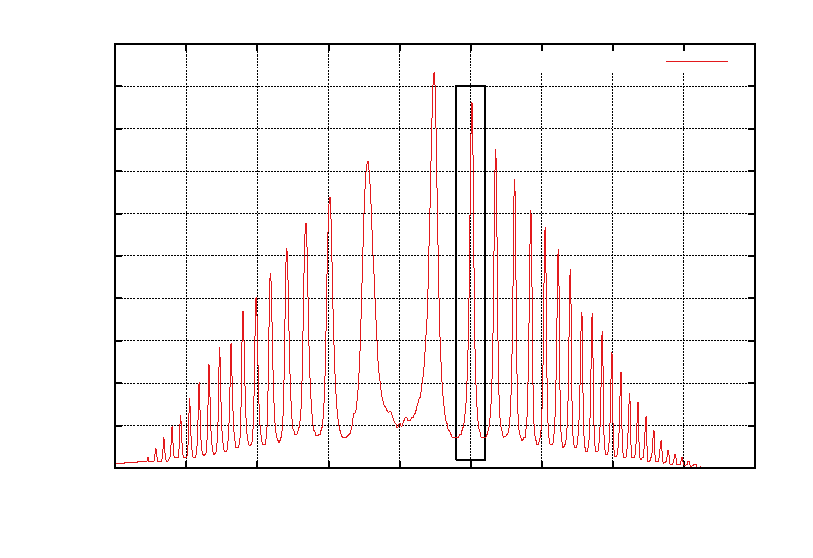
\includegraphics{./plots/peakauswahl}}%
    \gplfronttext
  \end{picture}%
\endgroup

	\caption{Intensitätsverteilung des Fabry-Pérot-Etalons bei abgeschaltetem Magnetfeld. Das in schwarz markierte Maximum wird zur Bestimmung des Magnetons verwendet.}
	\label{fig:peakauswahl}
\end{figure}
Zur Bestimmung des Bohrschen Magnetons müssen wir die Energieaufspaltung $\Delta E$ der Linie von Cadmium vermessen.
Dazu betrachten wir die mit der CCD-Kamera aufgenommenen Intensitäten eines inneren Rings bei variablem Spulenstrom $I$.
Der zur Analyse herangezogene Ring wurde in Abbildung \ref{fig:peakauswahl} markiert.
Um die Peakschwerpunkte der Aufspaltung zu vermessen passen wir an die Intensitätsverteilung des gewählten Rings eine Summe von drei Gaußfunktionen $\mathcal{G}$ mit Verschiebung $d$ an.
Die Anpassungshypothese lautet:
\begin{align}
f(x) = \mathcal{G}_1(x) + \mathcal{G}_2(x) + \mathcal{G}_3(x) + d
\end{align}
mit der Gaußfunktion:
\begin{align}
\mathcal{G}_i(x) = A_i \exp\left( -\frac{1}{2} \left( \frac{x - \mu_i}{\sigma_i} \right)^2 \right)
\end{align}
Wir erhalten als Anpassungsparameter die drei Höhen $A_i$, drei Peakschwerpunkte $\mu_i$, drei Standardabweichungen $\sigma_i$ und den konstanten Versatz $d$.
Zur Anpassung verwenden wir die Methode der kleinsten Quadrate (\texttt{GNUPlot}) und erhalten so beispielsweise für $B = \SI{4}{\tesla}$ Abbildung \ref{fig:zeeman_b4_bsp}.
\begin{figure}[h]
	\centering
	% GNUPLOT: LaTeX picture with Postscript
\begingroup
  \makeatletter
  \providecommand\color[2][]{%
    \GenericError{(gnuplot) \space\space\space\@spaces}{%
      Package color not loaded in conjunction with
      terminal option `colourtext'%
    }{See the gnuplot documentation for explanation.%
    }{Either use 'blacktext' in gnuplot or load the package
      color.sty in LaTeX.}%
    \renewcommand\color[2][]{}%
  }%
  \providecommand\includegraphics[2][]{%
    \GenericError{(gnuplot) \space\space\space\@spaces}{%
      Package graphicx or graphics not loaded%
    }{See the gnuplot documentation for explanation.%
    }{The gnuplot epslatex terminal needs graphicx.sty or graphics.sty.}%
    \renewcommand\includegraphics[2][]{}%
  }%
  \providecommand\rotatebox[2]{#2}%
  \@ifundefined{ifGPcolor}{%
    \newif\ifGPcolor
    \GPcolortrue
  }{}%
  \@ifundefined{ifGPblacktext}{%
    \newif\ifGPblacktext
    \GPblacktexttrue
  }{}%
  % define a \g@addto@macro without @ in the name:
  \let\gplgaddtomacro\g@addto@macro
  % define empty templates for all commands taking text:
  \gdef\gplbacktext{}%
  \gdef\gplfronttext{}%
  \makeatother
  \ifGPblacktext
    % no textcolor at all
    \def\colorrgb#1{}%
    \def\colorgray#1{}%
  \else
    % gray or color?
    \ifGPcolor
      \def\colorrgb#1{\color[rgb]{#1}}%
      \def\colorgray#1{\color[gray]{#1}}%
      \expandafter\def\csname LTw\endcsname{\color{white}}%
      \expandafter\def\csname LTb\endcsname{\color{black}}%
      \expandafter\def\csname LTa\endcsname{\color{black}}%
      \expandafter\def\csname LT0\endcsname{\color[rgb]{1,0,0}}%
      \expandafter\def\csname LT1\endcsname{\color[rgb]{0,1,0}}%
      \expandafter\def\csname LT2\endcsname{\color[rgb]{0,0,1}}%
      \expandafter\def\csname LT3\endcsname{\color[rgb]{1,0,1}}%
      \expandafter\def\csname LT4\endcsname{\color[rgb]{0,1,1}}%
      \expandafter\def\csname LT5\endcsname{\color[rgb]{1,1,0}}%
      \expandafter\def\csname LT6\endcsname{\color[rgb]{0,0,0}}%
      \expandafter\def\csname LT7\endcsname{\color[rgb]{1,0.3,0}}%
      \expandafter\def\csname LT8\endcsname{\color[rgb]{0.5,0.5,0.5}}%
    \else
      % gray
      \def\colorrgb#1{\color{black}}%
      \def\colorgray#1{\color[gray]{#1}}%
      \expandafter\def\csname LTw\endcsname{\color{white}}%
      \expandafter\def\csname LTb\endcsname{\color{black}}%
      \expandafter\def\csname LTa\endcsname{\color{black}}%
      \expandafter\def\csname LT0\endcsname{\color{black}}%
      \expandafter\def\csname LT1\endcsname{\color{black}}%
      \expandafter\def\csname LT2\endcsname{\color{black}}%
      \expandafter\def\csname LT3\endcsname{\color{black}}%
      \expandafter\def\csname LT4\endcsname{\color{black}}%
      \expandafter\def\csname LT5\endcsname{\color{black}}%
      \expandafter\def\csname LT6\endcsname{\color{black}}%
      \expandafter\def\csname LT7\endcsname{\color{black}}%
      \expandafter\def\csname LT8\endcsname{\color{black}}%
    \fi
  \fi
  \setlength{\unitlength}{0.0500bp}%
  \begin{picture}(7486.00,5040.00)%
    \gplgaddtomacro\gplbacktext{%
      \csname LTb\endcsname%
      \put(814,704){\makebox(0,0)[r]{\strut{} 0}}%
      \csname LTb\endcsname%
      \put(814,1156){\makebox(0,0)[r]{\strut{} 5}}%
      \csname LTb\endcsname%
      \put(814,1609){\makebox(0,0)[r]{\strut{} 10}}%
      \csname LTb\endcsname%
      \put(814,2061){\makebox(0,0)[r]{\strut{} 15}}%
      \csname LTb\endcsname%
      \put(814,2513){\makebox(0,0)[r]{\strut{} 20}}%
      \csname LTb\endcsname%
      \put(814,2966){\makebox(0,0)[r]{\strut{} 25}}%
      \csname LTb\endcsname%
      \put(814,3418){\makebox(0,0)[r]{\strut{} 30}}%
      \csname LTb\endcsname%
      \put(814,3870){\makebox(0,0)[r]{\strut{} 35}}%
      \csname LTb\endcsname%
      \put(814,4323){\makebox(0,0)[r]{\strut{} 40}}%
      \csname LTb\endcsname%
      \put(814,4775){\makebox(0,0)[r]{\strut{} 45}}%
      \csname LTb\endcsname%
      \put(946,484){\makebox(0,0){\strut{} 0.8}}%
      \csname LTb\endcsname%
      \put(1714,484){\makebox(0,0){\strut{} 0.85}}%
      \csname LTb\endcsname%
      \put(2482,484){\makebox(0,0){\strut{} 0.9}}%
      \csname LTb\endcsname%
      \put(3250,484){\makebox(0,0){\strut{} 0.95}}%
      \csname LTb\endcsname%
      \put(4018,484){\makebox(0,0){\strut{} 1}}%
      \csname LTb\endcsname%
      \put(4785,484){\makebox(0,0){\strut{} 1.05}}%
      \csname LTb\endcsname%
      \put(5553,484){\makebox(0,0){\strut{} 1.1}}%
      \csname LTb\endcsname%
      \put(6321,484){\makebox(0,0){\strut{} 1.15}}%
      \csname LTb\endcsname%
      \put(7089,484){\makebox(0,0){\strut{} 1.2}}%
      \put(176,2739){\rotatebox{-270}{\makebox(0,0){\strut{}Intensität $I$ / \si{\percent}}}}%
      \put(4017,154){\makebox(0,0){\strut{}Winkel $\alpha$ / \si{\degree}}}%
      \put(4017,4665){\makebox(0,0){\strut{}}}%
    }%
    \gplgaddtomacro\gplfronttext{%
      \csname LTb\endcsname%
      \put(6102,4602){\makebox(0,0)[r]{\strut{}Messwerte}}%
      \csname LTb\endcsname%
      \put(6102,4382){\makebox(0,0)[r]{\strut{}Summe Gaußfits}}%
      \csname LTb\endcsname%
      \put(6102,4162){\makebox(0,0)[r]{\strut{}Funktion 1}}%
      \csname LTb\endcsname%
      \put(6102,3942){\makebox(0,0)[r]{\strut{}Funktion 2}}%
      \csname LTb\endcsname%
      \put(6102,3722){\makebox(0,0)[r]{\strut{}Funktion 3}}%
      \csname LTb\endcsname%
      \put(6102,3502){\makebox(0,0)[r]{\strut{}Untergrund}}%
    }%
    \gplbacktext
    \put(0,0){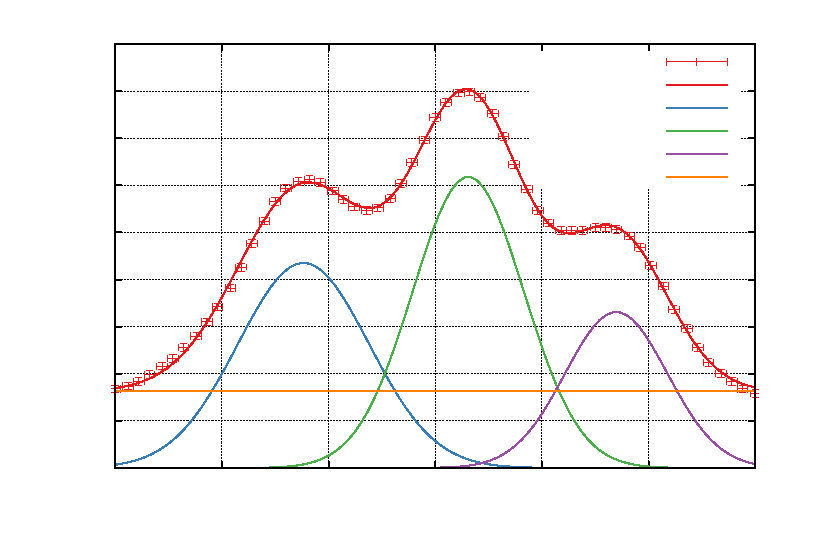
\includegraphics{./plots/zeemann_aufspaltung/b4}}%
    \gplfronttext
  \end{picture}%
\endgroup

	\caption{Beispiel zur Anpassung der Gaußfunktionen an die Aufspaltung (hier $B = \SI{4}{\tesla}$). $\mathcal{G}_1$: $\sigma_-$-Linie;\, $\mathcal{G}_2$: $\pi$-Linie;\, $\mathcal{G}_3$: $\sigma_+$-Linie; $d$: Verschiebung;\, $\Sigma$: Summe von Gaußfunktionen und Verschiebung}
	\label{fig:zeeman_b4_bsp}
\end{figure}
Die restlichen Anpassungen finden sich in Anhang \ref{app:penis}.
Die Ergebnisse für die Schwerpunkte der einzelnen Linien finden sich in Tabelle \ref{tab:peakschwerpunkte_magneton}.

\begin{table}[h]
	\centering
	\resizebox{\columnwidth}{!}{%
		\begin{tabular}{SSSSSSS}
\toprule
{Strom $I$ / \si{\ampere}} & {$\alpha_-$ / \si{\milli\degree}}& {$\sigma_{\alpha_-}$ / \si{\milli\degree}}& {$\alpha_0$ / \si{\milli\degree}} &{$\sigma_{\alpha_0}$ / \si{\milli\degree}} & {$\alpha_+$ / \si{\milli\degree}} & {$\sigma_{\alpha_+}$ / \si{\milli\degree}}\\
\midrule
4.0	&	938.25&	0.59	&		1015.47&	0.31	&		1084.82&	0.62	\\
4.5	&	926.15&	0.35	&		1013.00&	0.23	&		1091.78&	0.48	\\
5.0	&	915.79&	0.45	&		1011.60&	0.31	&		1098.57&	0.58	\\
5.5	&	907.63&	0.43	&		1010.37&	0.31	&		1103.19&	0.56	\\
6.0	&	899.42&	0.56	&		1009.48&	0.38	&		1108.59&	0.73	\\
6.5	&	892.78&	0.64	&		1008.75&	0.43	&		1113.06&	0.84	\\
7.0	&	887.92&	0.72	&		1007.77&	0.48	&		1115.89&	1.00	\\
7.5	&	883.05&	0.83	&		1007.17&	0.55	&		1119.34&	1.24	\\
8.0	&	879.59&	0.83	&		1006.73&	0.48	&		1120.66&	1.13	\\
8.5	&	874.79&	0.75	&		1005.64&	0.47	&		1122.76&	1.13	\\
8.9	&	871.95&	0.75	&		1005.28&	0.39	&		1123.36&	0.96	\\
\bottomrule
\end{tabular}}
	\caption{Durch Kurvenanpassung bestimmte Schwerpunkte $\alpha_i$ (in Milligrad) der drei Linien. Der Fehler des Spulenstroms $I$ ist gegeben durch $\sigma_I = \SI{0.1}{\ampere}$.}
	\label{tab:peakschwerpunkte_magneton}
\end{table}

Mithilfe der so berechneten Peakschwerpunkte können wir die relative Abweichung von der $\pi$-Linie berechnen.
Dazu nutzen wir die Interferenzbedingung für das Fabry-Pérot-Etalon aus Gleichung \ref{eq:interferenzbedingung} und erhalten:
\begin{align}
	\frac{\Delta \lambda_\pm}{\lambda_\pi^0} = \frac{\lambda_{\sigma^\pm} - \lambda_\pi^0}{\lambda_\pi^0} = \frac{\sqrt{n^2 - \sin^2(\alpha_{\pm})}}{\sqrt{n^2 - \sin^2(\alpha_\pi)}} - 1
\end{align}
Dabei berechnet sich der  Fehler über Gaußscher Fehlerfortpflanzung zu:
\begin{align}
	\Delta \left( \frac{\Delta \lambda_\pm}{\lambda_\pi^0} \right) = & \left( \frac{\sin^2(\alpha_\pm) \cos^2(\alpha_\pm)}{(n^2-\sin^2(\alpha_\pm))(n^2-\sin^2(\alpha_\pi))} \cdot \Delta \alpha_\pm^2 \right. \nonumber\\
	& \left. + \frac{\sin^2(\alpha_\pi) \cos^2(\alpha_\pi) (n^2 - \sin^2(\alpha_\pm))}{(n^2-\sin^2(\alpha_\pi))^3} \cdot \Delta \alpha_\pi^2\right)^\frac{1}{2}
\end{align}
Mit diesen Gleichungen folgen für die relative Abweichung die Werte der Tabelle \ref{tab:verschiebung_wellenlaenge}. 
\begin{table}[h]
	\centering
	\begin{tabular}{SSSSS}
\toprule
{$I$ / \si{\ampere}} & {$\frac{\Delta \lambda_{-}}{\lambda_\pi^0}$} & {$\sigma_\mathrm{rel.}^{-}$} & {$\frac{\Delta \lambda_{+}}{\lambda_\pi^0}$} & {$\sigma_\mathrm{rel.}^{+}$} \\
\midrule
4.0 & 1.0824 & 0.0090 & -1.0450 & 0.0107 \\
4.5 & 1.2083 & 0.0058 & -1.1896 & 0.0080 \\
5.0 & 1.3249 & 0.0074 & -1.3166 & 0.0102 \\
5.5 & 1.4138 & 0.0071 & -1.4074 & 0.0099 \\
6.0 & 1.5072 & 0.0091 & -1.5060 & 0.0128 \\
6.5 & 1.5822 & 0.0102 & -1.5878 & 0.0147 \\
7.0 & 1.6300 & 0.0139 & -1.6473 & 0.0174 \\
7.5 & 1.6832 & 0.0132 & -1.7113 & 0.0215 \\
8.0 & 1.7206 & 0.0125 & -1.7388 & 0.0194 \\
8.5 & 1.7654 & 0.0116 & -1.7884 & 0.0193 \\
8.9 & 1.7957 & 0.0109 & -1.8032 & 0.0164 \\
\bottomrule
\end{tabular}
	\caption{Relative Wellenlängenverschiebung zur $\pi$-Linie aus den angepassten Schwerpunkten der Tabelle \ref{tab:peakschwerpunkte_magneton}. Fehler des Spulenstroms: $\sigma_I = \SI{0.1}{\ampere}$.}
	\label{tab:verschiebung_wellenlaenge}
\end{table}
Mit der Wellenlänge der $\pi$-Linie\footnote{National Institute of Standards and Technology (NIST)\\ \url{http://physics.nist.gov/PhysRefData/Handbook/Tables/cadmiumtable2.htm}\\Letzter Aufruf: 22. November 2014} $\lambda_\pi = \SI{643,8470}{\nano\metre}$  und der relativen Wellenlängenverschiebung kann nun die Energieaufspaltung $\Delta E$ der Ringe berechnet werden:
\begin{align}
	\Delta E = -\frac{h c}{\lambda_\pi^0}\,\frac{\Delta \lambda}{\lambda_{\sigma^\pm}} \approx -\frac{h c}{\lambda_\pi^0}\,\frac{\Delta \lambda}{\lambda_\pi^0} \text{,}
\end{align}
wobei der Fehler aus Gaußscher Fehlerfortpflanzung folgt:
\begin{align}
	\sigma_{\Delta E} = \frac{h c}{\lambda_\pi^0} \, | \sigma_{\Delta \lambda / \lambda_\pi^0} |
\end{align}
Die Energieaufspaltung wurde für die verschiedenen Spulenströme in Tabelle \ref{tab:energieaufspaltung} dargestellt.
\begin{table}[h]
	\centering
	\begin{tabular}{SSSSS}
\toprule
{Strom $I$ / \si{\ampere}} & {$\Delta E_{-}$ / \si{\electronvolt}} & {$\sigma_{\Delta E_{-}}$ / \si{\electronvolt}} & {$\Delta E_{+}$ / \si{\electronvolt}} & {$\sigma_{\Delta E_{+}}$ / \si{\electronvolt}} \\
\midrule
4.0 & -2.084 & 0.018 & 2.012 & 0.021 \\
4.5 & -2.327 & 0.011 & 2.291 & 0.016 \\
5.0 & -2.551 & 0.015 & 2.535 & 0.020 \\
5.5 & -2.723 & 0.014 & 2.710 & 0.020 \\
6.0 & -2.902 & 0.018 & 2.900 & 0.025 \\
6.5 & -3.047 & 0.020 & 3.058 & 0.029 \\
7.0 & -3.139 & 0.022 & 3.172 & 0.034 \\
7.5 & -3.241 & 0.026 & 3.295 & 0.042 \\
8.0 & -3.313 & 0.024 & 3.348 & 0.038 \\
8.5 & -3.400 & 0.023 & 3.444 & 0.038 \\
8.9 & -3.458 & 0.021 & 3.472 & 0.032 \\
\bottomrule
\end{tabular}
	\caption{Energieaufspaltung der $\sigma_\pm$-Linien bei anliegendem Spulenstrom $I$ ($\sigma_I = \SI{0.1}{\ampere}$).}
	\label{tab:energieaufspaltung}
\end{table}
Diese ist gemäß des normalen Zeeman-Effektes (Gleichung \ref{eq:normaler_zeeman}) gegeben durch:
\begin{align}
	\Delta E = \mu_\mathrm{B} \Delta m_\ell B
	\label{eq:normaler_zeeman_auswertung}
\end{align}
Wenn man $\Delta E$ gegen $B$ aufträgt so erhält man eine Gerade mit Steigung $\pm \mu_\mathrm{B}$.
Dazu müssen wir zunächst das Magnetfeld $B$ mit der Kalibrierung aus den Spulenströmen berechnen.
Da die beiden Kalibrierungen eine kleine Abweichung im Bereich hoher Ströme aufweisen, entscheiden wir uns dafür ein mittleres Magnetfeld durch Anwendung des ungewichteten arithmetischen Mittels auf die beiden berechneten Feldstärken zu berechnen.
Wir verwenden dabei den ungewichteten Mittelwert, da die Fehler der beiden Feldstärken nahezu gleich sind.
Der Fehler des Mittelwerts von zwei Größen ergibt sich dann aus: $\sigma_{\bar{B}} = \frac{\sigma_\mathrm{max.}}{\sqrt{2}}$, wobei wir für $\sigma_\mathrm{max.}$ stets den größeren ($\sigma_\mathrm{max.} = \max(\sigma_{B_1}, \sigma_{B_2}) $) der beiden Fehler verwenden.
Die zu den gemessenen Spulenströmen korrespondierenden Magnetfelder wurden in Tabelle \ref{tab:mittelwert_kalibration} aufgetragen, wobei die Fehler der Anpassungsparameter und der Spulenströme\footnote{Für die Spulenströme wurde ein Fehler von $\sigma_I = \SI{0.1}{\ampere}$ angenommen, was der Stelle der niedrigsten Wertigkeit auf der digitalen Anzeige des Netzgerätes entspricht.} der Kalibration bei der Berechnung der Magnetfelder $B_1, B_2$ durch Gaußsche Fehlerfortpflanzung beachtet wurden.
\begin{table}[h]
	\centering
	\begin{tabular}{SSSSSSS}
\toprule
{Strom $I$ / \si{\ampere}} & {$B_1$} & {$\sigma_{B_1}$} & {$B_2$} & {$\sigma_{B_2}$} & {$\bar{B}$} & {$\sigma_{\bar{B}}$}\\
\midrule
4.0 & 373.5 & 4.0 & 373.6 & 4.0 & 373.6 & 2.8\\
4.5 & 414.5 & 4.9 & 415.3 & 4.8 & 414.9 & 3.4\\
5.0 & 453.1 & 5.8 & 454.5 & 5.8 & 453.8 & 4.1\\
5.5 & 489.3 & 6.9 & 490.9 & 6.9 & 490.1 & 4.9\\
6.0 & 522.6 & 8.1 & 524.2 & 8.1 & 523.4 & 5.7\\
6.5 & 552.8 & 9.5 & 553.8 & 9.5 & 553.3 & 6.7\\
7.0 & 579.6 & 10.9 & 579.5 & 11.0 & 579.5 & 7.8\\
7.5 & 602.7 & 12.6 & 600.8 & 12.7 & 601.7 & 8.9\\
8.0 & 621.7 & 14.4 & 617.3 & 14.5 & 619.5 & 10.2\\
8.5 & 636.5 & 16.4 & 628.7 & 16.5 & 632.7 & 11.6\\
8.9 & 645.1 & 18.1 & 633.9 & 18.3 & 639.6 & 12.9\\
\bottomrule
\end{tabular}
	\caption{Stromkalib}
	\label{tab:mittelwert_kalibration}
\end{table}

Wir tragen nun den Betrag der Energieaufspaltung $|\Delta E|$ für die $\sigma_-$- und $\sigma_+$-Linien gegen das anliegende Magnetfeld $\bar{B}$ auf und passen eine Ursprungsgeraden an.
Wir erhalten für die Ursprungsgeraden:
\begin{align}
	|\Delta E_{-}| = \SI{5.502 +- 0.031e-5}{\electronvolt\per\tesla} \cdot \bar{B} \qquad \chi_\mathrm{d.o.f.}^2 = 8.94\\
	|\Delta E_{+}| = \SI{5.497 +- 0.019e-5}{\electronvolt\per\tesla} \cdot \bar{B} \qquad \chi_\mathrm{d.o.f.}^2 = 1.62
\end{align}
\begin{figure}[h]
	\centering
	% GNUPLOT: LaTeX picture with Postscript
\begingroup
  \makeatletter
  \providecommand\color[2][]{%
    \GenericError{(gnuplot) \space\space\space\@spaces}{%
      Package color not loaded in conjunction with
      terminal option `colourtext'%
    }{See the gnuplot documentation for explanation.%
    }{Either use 'blacktext' in gnuplot or load the package
      color.sty in LaTeX.}%
    \renewcommand\color[2][]{}%
  }%
  \providecommand\includegraphics[2][]{%
    \GenericError{(gnuplot) \space\space\space\@spaces}{%
      Package graphicx or graphics not loaded%
    }{See the gnuplot documentation for explanation.%
    }{The gnuplot epslatex terminal needs graphicx.sty or graphics.sty.}%
    \renewcommand\includegraphics[2][]{}%
  }%
  \providecommand\rotatebox[2]{#2}%
  \@ifundefined{ifGPcolor}{%
    \newif\ifGPcolor
    \GPcolortrue
  }{}%
  \@ifundefined{ifGPblacktext}{%
    \newif\ifGPblacktext
    \GPblacktexttrue
  }{}%
  % define a \g@addto@macro without @ in the name:
  \let\gplgaddtomacro\g@addto@macro
  % define empty templates for all commands taking text:
  \gdef\gplbacktext{}%
  \gdef\gplfronttext{}%
  \makeatother
  \ifGPblacktext
    % no textcolor at all
    \def\colorrgb#1{}%
    \def\colorgray#1{}%
  \else
    % gray or color?
    \ifGPcolor
      \def\colorrgb#1{\color[rgb]{#1}}%
      \def\colorgray#1{\color[gray]{#1}}%
      \expandafter\def\csname LTw\endcsname{\color{white}}%
      \expandafter\def\csname LTb\endcsname{\color{black}}%
      \expandafter\def\csname LTa\endcsname{\color{black}}%
      \expandafter\def\csname LT0\endcsname{\color[rgb]{1,0,0}}%
      \expandafter\def\csname LT1\endcsname{\color[rgb]{0,1,0}}%
      \expandafter\def\csname LT2\endcsname{\color[rgb]{0,0,1}}%
      \expandafter\def\csname LT3\endcsname{\color[rgb]{1,0,1}}%
      \expandafter\def\csname LT4\endcsname{\color[rgb]{0,1,1}}%
      \expandafter\def\csname LT5\endcsname{\color[rgb]{1,1,0}}%
      \expandafter\def\csname LT6\endcsname{\color[rgb]{0,0,0}}%
      \expandafter\def\csname LT7\endcsname{\color[rgb]{1,0.3,0}}%
      \expandafter\def\csname LT8\endcsname{\color[rgb]{0.5,0.5,0.5}}%
    \else
      % gray
      \def\colorrgb#1{\color{black}}%
      \def\colorgray#1{\color[gray]{#1}}%
      \expandafter\def\csname LTw\endcsname{\color{white}}%
      \expandafter\def\csname LTb\endcsname{\color{black}}%
      \expandafter\def\csname LTa\endcsname{\color{black}}%
      \expandafter\def\csname LT0\endcsname{\color{black}}%
      \expandafter\def\csname LT1\endcsname{\color{black}}%
      \expandafter\def\csname LT2\endcsname{\color{black}}%
      \expandafter\def\csname LT3\endcsname{\color{black}}%
      \expandafter\def\csname LT4\endcsname{\color{black}}%
      \expandafter\def\csname LT5\endcsname{\color{black}}%
      \expandafter\def\csname LT6\endcsname{\color{black}}%
      \expandafter\def\csname LT7\endcsname{\color{black}}%
      \expandafter\def\csname LT8\endcsname{\color{black}}%
    \fi
  \fi
  \setlength{\unitlength}{0.0500bp}%
  \begin{picture}(7488.00,5040.00)%
    \gplgaddtomacro\gplbacktext{%
      \csname LTb\endcsname%
      \put(946,704){\makebox(0,0)[r]{\strut{} 0}}%
      \csname LTb\endcsname%
      \put(946,1156){\makebox(0,0)[r]{\strut{} 0.5}}%
      \csname LTb\endcsname%
      \put(946,1609){\makebox(0,0)[r]{\strut{} 1}}%
      \csname LTb\endcsname%
      \put(946,2061){\makebox(0,0)[r]{\strut{} 1.5}}%
      \csname LTb\endcsname%
      \put(946,2513){\makebox(0,0)[r]{\strut{} 2}}%
      \csname LTb\endcsname%
      \put(946,2966){\makebox(0,0)[r]{\strut{} 2.5}}%
      \csname LTb\endcsname%
      \put(946,3418){\makebox(0,0)[r]{\strut{} 3}}%
      \csname LTb\endcsname%
      \put(946,3870){\makebox(0,0)[r]{\strut{} 3.5}}%
      \csname LTb\endcsname%
      \put(946,4323){\makebox(0,0)[r]{\strut{} 4}}%
      \csname LTb\endcsname%
      \put(946,4775){\makebox(0,0)[r]{\strut{} 4.5}}%
      \csname LTb\endcsname%
      \put(1078,484){\makebox(0,0){\strut{} 350}}%
      \csname LTb\endcsname%
      \put(1937,484){\makebox(0,0){\strut{} 400}}%
      \csname LTb\endcsname%
      \put(2796,484){\makebox(0,0){\strut{} 450}}%
      \csname LTb\endcsname%
      \put(3655,484){\makebox(0,0){\strut{} 500}}%
      \csname LTb\endcsname%
      \put(4514,484){\makebox(0,0){\strut{} 550}}%
      \csname LTb\endcsname%
      \put(5373,484){\makebox(0,0){\strut{} 600}}%
      \csname LTb\endcsname%
      \put(6232,484){\makebox(0,0){\strut{} 650}}%
      \csname LTb\endcsname%
      \put(7091,484){\makebox(0,0){\strut{} 700}}%
      \put(176,2739){\rotatebox{-270}{\makebox(0,0){\strut{}E / $10^{-5} \si{\electronvolt}$}}}%
      \put(4084,154){\makebox(0,0){\strut{}B / $\si{\milli\tesla}$}}%
      \put(4084,4665){\makebox(0,0){\strut{}}}%
    }%
    \gplgaddtomacro\gplfronttext{%
      \csname LTb\endcsname%
      \put(2398,4602){\makebox(0,0)[r]{\strut{}E-}}%
      \csname LTb\endcsname%
      \put(2398,4382){\makebox(0,0)[r]{\strut{}E+}}%
      \csname LTb\endcsname%
      \put(2398,4162){\makebox(0,0)[r]{\strut{}E-}}%
      \csname LTb\endcsname%
      \put(2398,3942){\makebox(0,0)[r]{\strut{}E+}}%
      \csname LTb\endcsname%
      \put(2398,3722){\makebox(0,0)[r]{\strut{}Literatur}}%
    }%
    \gplbacktext
    \put(0,0){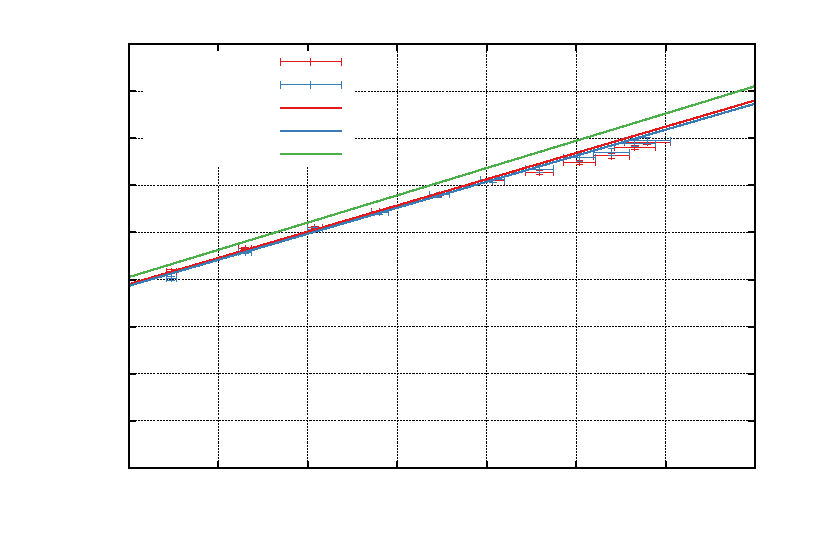
\includegraphics{./plots/magneton_fit}}%
    \gplfronttext
  \end{picture}%
\endgroup

	\caption{magneton fit}
	\label{fig:magneton_fit}
\end{figure}
Gemäß Gleichung \ref{eq:normaler_zeeman_auswertung} entspricht die Steigung der Ursprungsgeraden im $|\Delta E|$-$\bar{B}$-Graph dem Bohrschen Magneton. Zur Bestimmung des Bohrschen Magnetons berechnen wir das varianzgewichtete Mittel der beiden Steigungen:
\begin{align}
	\bar{x} = \frac{\sum_i \frac{x_i}{\sigma_i^2}}{\sum_i \frac{1}{\sigma_i^2}}\text{,}
\end{align}
wobei der Fehler des gewichteten Mittelwerts gegeben ist durch:
\begin{align}
	\sigma_{\bar{x}} = \frac{1}{\sqrt{\sum_i \frac{1}{\sigma_i^2}}}\text{.}
\end{align}
Damit erhalten wir für das Bohrsche Magneton:
\begin{align}
	\mu_\mathrm{B} = \SI{5.498 +- 0.017e-5}{\electronvolt\per\tesla}
\end{align}

Vergleich mit dem Literaturwert\footnote{2010 CODATA recommended values\\ \url{http://physics.nist.gov/cgi-bin/cuu/Value?mubev}\\ Letzter Abruf: 24. November 2014}.
\begin{align}
	\mu_\mathrm{B}^{\mathrm{Lit.}} = \SI{5.7883818066 +- 0.0000000038e-5}{\electronvolt\per\tesla}
\end{align}



\subsubsection{Weitergehende Überlegungen}
\textbf{Abschätzung des Auflösungsvermögens $\mathcal{R}$ und der Finesse $\mathcal{F}$ des Fabry-Pérot-Etalons}:
Zunächst wollen wir das theoretische Auflösungsvermögen und Finesse des Etalons berechnen.
Diese lassen sich mit Gleichung \ref{eq:finesse} und \ref{eq:aufloesung} des Grundlagenteils aus dem Reflektionskoeffizienten $r$ und der Ordnung $m$ des Interferenzrings berechnen.
Mit dem gegebenen Wert $r = \num{0,85}$ folgt unmittelbar für die Finesse:
\begin{align*}
	\mathcal{F_\mathrm{theo.}} = \frac{\pi r}{1 - r^2} \approx \num{9.62}
\end{align*}
Zur Berechnung des Auflösungsvermögen $\mathcal{R}$ nutzen wir den Zusammenhang mit der Finesse $\mathcal{F}$:
\begin{align}
\mathcal{R} = \mathcal{F} \cdot m
\end{align}
Dazu schätzen wir die Ordnung $m$ mit der Interferenzbedingung des Fabry-Pérot-Etalons ab:
\begin{align*}
m = \frac{2 d}{\lambda} \sqrt{n^2 - \sin^2(\alpha)} \approx \frac{2 d n}{\lambda} \approx 18104
\end{align*}
Es folgt für das theoretische Auflösungsvermögen:
\begin{align*}
	\mathcal{R}_\mathrm{theo.} = \mathcal{F}_\mathrm{theo.} \cdot m  \approx \num{174000}
\end{align*}

\begin{table}[h]
	\centering
	\begin{tabular}{lSS}
\toprule
{\#} & {$I_\mathrm{trans.} / \si{\ampere}$} & {$I_\mathrm{long.} / \si{\ampere}$}\\
\midrule
1&	2.1 +- 0.1&	1.1 +- 0.1 \\
2&	2.1 +- 0.1&	1.0 +- 0.1 \\
3&	2.0 +- 0.1&	1.1 +- 0.1 \\
4&	2.0 +- 0.1&	1.1 +- 0.1 \\
5&	2.0 +- 0.1&	1.0 +- 0.1 \\
\bottomrule
\end{tabular}
	\caption{Messdaten zur Bestimmung der Auflösung und Finesse mit dem Okular}
	\label{tab:aufloesung}
\end{table}
Nun wollen wir aus den Spulenströmen bei denen aufgespaltene Ringe im Okular gerade noch zu unterscheiden waren (Tabelle \ref{tab:aufloesung}) die Finesse und das Auflösungsvermögen berechnen.
Um den Messfehler besser einschätzen zu können, wurde in jeder Konfiguration fünf mal gemessen.
Es wurde jeweils ein Fehler von $\SI{0.1}{\ampere}$ auf den am Netzgerät abgelesenen Spulenstrom angenommen, da dies der niedrigstwertigen Stelle an der digitalen Anzeige entspricht.
Da der Fehler für alle fünf Messungen gleich ist ergibt sich der Fehler des Mittelwerts aus: 
\begin{align*}
	\sigma_{\bar{I}} = \frac{\sigma_I}{\sqrt{N}} = \frac{\SI{0,1}{\ampere}}{\sqrt{5}} \approx \SI{0,045}{\ampere}\text{.}
\end{align*}
Damit erhalten wir nach der Mittelwertbildung:
\begin{align*}
	\bar{I}_\mathrm{trans.} = \SI{2.040 +- 0.045}{\ampere} \\
	\bar{I}_\mathrm{long.} = \SI{1.060 +- 0.045}{\ampere}\text{.}
\end{align*}
Zur Bestimmung der Auflösung muss zunächst das aus dem Spulenstrom $\bar{I}$ resultierende Magnetfeld aus der Kalibrierung berechnet werden.
Dazu gehen wir analog zum vorigen Teil vor und berechnen mit die Feldstärke mit beiden Kalibrierungen und mitteln deren Werte.
Wir beachten die Fehler in $\bar{I}$ und in den Anpassungsparametern des Polynoms durch Gaußsche Fehlerfortpflanzung und erhalten:
\begin{align*}
	B_\mathrm{trans.} = \SI{195.6 +- 3.3}{\milli\tesla} \\
	B_\mathrm{long.} = \SI{101.6 +- 3.2}{\milli\tesla}
\end{align*}
Die Auflösung ist nun gegeben durch Gleichung \ref{eq:aufloesung}, wobei $\delta \lambda$ die Halbwertsbreite der Intensitätsmaxima des Fabry-Pérot-Etalon ist.
Gemäß des Rayleigh-Kriteriums sind zwei Linien $(\lambda_1, \lambda_2)$ gerade noch aufgelöst, wenn deren Wellenlängenunterschied $\lambda_2 - \lambda_1$ gleich der Halbwertsbreite $\delta \lambda$ des Intensitätsprofils einer einzigen Linie ist.
Damit können wir die Halbwertsbreite $\delta \lambda$ der Intensitätsspitzen des Etalons durch die Wellenlängendifferenz zweier gerade noch aufgelösten Linien bestimmen, welche durch die Energieaufspaltung $\Delta E$ aufgrund des normalen Zeeman-Effekts entsteht:
\begin{align}
	\delta \lambda = \lambda_2 - \lambda_1 = h c \left( \frac{1}{E_2} - \frac{1}{E_1} \right) = \frac{h c}{E_1 E_2} \left(E_1 - E_2\right) \approx \frac{\lambda^2 \cdot \Delta E}{h c}
\end{align}
wobei im letzten Schritt die Näherung $\lambda \approx \lambda_1 \approx \lambda_2$ verwendet wurde.
Dann ist die Auflösung gegeben durch:
\begin{align}
	\mathcal{R} = \frac{\lambda}{\delta \lambda} = \frac{h c}{\lambda \cdot \Delta E}\text{,}
\end{align}
wobei die Energieaufspaltung durch den normalen Zeemaneffekt in Abhängigkeit vom anliegenden Magnetfeld $B$:
\begin{align}
	\Delta E = \mu_\mathrm{B} \Delta m B
\end{align}
gegeben ist.
Also folgt für das Auflösungsvermögen
\begin{align}
	\mathcal{R} = \frac{h c}{ \mu_\mathrm{B} \Delta m \lambda} \cdot \frac{1}{B} 
\end{align}
und für den Fehler nach Gaußscher Fehlerfortpflanzung::
\begin{align}
	\Delta \mathcal{R} = \frac{h c}{ \mu_\mathrm{B} \Delta m \lambda} \cdot \frac{\Delta B}{B^2} \text{.}
\end{align}
Mit diesen Überlegungen ergibt sich für die transversale Auflösung mit $\Delta m = 1$, da die Aufspaltung zwischen $\sigma_\pm$-Linie und $\pi$-Linie beobachtet wird und für die longitudinale Auflösung mit $\Delta m = 2$, da hier die Aufspaltung zwischen $\sigma_-$- und $\sigma_+$-Linie beobachtet wird ($\pi$-Linie ist in longitudinaler Konfiguration nicht sichtbar), gegeben durch:
\begin{align*}
	\mathcal{R}_\mathrm{trans.} = \num{170000 +- 2900} \\
	\mathcal{R}_\mathrm{long.} =\num{164000 +- 5200}
\end{align*}
Diese Werte stimmen gut mit dem theoretischen Wert überein.
Die Unterschätzung bei der longitudinalen Konfiguration lässt sich dadurch erklären, dass die $\pi$-Linie im Okular noch leicht sichtbar war und dadurch eine Unterscheidung der $\sigma$-Linien aufgrund der dazwischenliegenden $\pi$-Linie schon bei größeren Spulenströmen nicht mehr möglich war.

Anschließend bestimmen wir die Finesse aus deren Zusammenhang mit dem Auflösungsvermögen:
\begin{align*}
\mathcal{R} = \mathcal{F} \cdot m \quad \rightarrow \quad \mathcal{F} = \frac{\mathcal{R}}{m}\text{,}                    
\end{align*}
wobei wir die Ordnung $m$ wieder durch $m \approx \num{18104}$ abschätzen und erhalten:
\begin{align*}
	\mathcal{F}_\mathrm{trans.} = \num{9.39 +- 0.17} \\
	\mathcal{F}_\mathrm{long.} = \num{9.06  +- 0.29}\text{,}
\end{align*}
was ebenfalls in Anbetracht der theoretischen Werte plausibel ist.

Schließlich soll Auflösungsvermögen und Finesse mithilfe der CCD-Kamera bestimmt werden.
Dazu muss im Wesentlichen die Breite eines Intensitätsmaximums des Fabry-Pérot-Etalons in der CCD-Aufnahme bestimmt werden.
Um diese zu bestimmen passen wir, ähnlich zu Abschnitt \ref{sssec:magneton}, eine Summe von Gaußfunktion $\mathcal{G}$ und konstanter Verschiebung $d$ an die Intensitätsdaten ohne externes Magnetfeld an.
Wir betrachten wieder das in Abbildung \ref{fig:peakauswahl} markierte Maximum und erhalten nach Anpassung die Abbildung \ref{fig:gauss0}.
\begin{figure}[h]
	\centering
	% GNUPLOT: LaTeX picture with Postscript
\begingroup
  \makeatletter
  \providecommand\color[2][]{%
    \GenericError{(gnuplot) \space\space\space\@spaces}{%
      Package color not loaded in conjunction with
      terminal option `colourtext'%
    }{See the gnuplot documentation for explanation.%
    }{Either use 'blacktext' in gnuplot or load the package
      color.sty in LaTeX.}%
    \renewcommand\color[2][]{}%
  }%
  \providecommand\includegraphics[2][]{%
    \GenericError{(gnuplot) \space\space\space\@spaces}{%
      Package graphicx or graphics not loaded%
    }{See the gnuplot documentation for explanation.%
    }{The gnuplot epslatex terminal needs graphicx.sty or graphics.sty.}%
    \renewcommand\includegraphics[2][]{}%
  }%
  \providecommand\rotatebox[2]{#2}%
  \@ifundefined{ifGPcolor}{%
    \newif\ifGPcolor
    \GPcolortrue
  }{}%
  \@ifundefined{ifGPblacktext}{%
    \newif\ifGPblacktext
    \GPblacktexttrue
  }{}%
  % define a \g@addto@macro without @ in the name:
  \let\gplgaddtomacro\g@addto@macro
  % define empty templates for all commands taking text:
  \gdef\gplbacktext{}%
  \gdef\gplfronttext{}%
  \makeatother
  \ifGPblacktext
    % no textcolor at all
    \def\colorrgb#1{}%
    \def\colorgray#1{}%
  \else
    % gray or color?
    \ifGPcolor
      \def\colorrgb#1{\color[rgb]{#1}}%
      \def\colorgray#1{\color[gray]{#1}}%
      \expandafter\def\csname LTw\endcsname{\color{white}}%
      \expandafter\def\csname LTb\endcsname{\color{black}}%
      \expandafter\def\csname LTa\endcsname{\color{black}}%
      \expandafter\def\csname LT0\endcsname{\color[rgb]{1,0,0}}%
      \expandafter\def\csname LT1\endcsname{\color[rgb]{0,1,0}}%
      \expandafter\def\csname LT2\endcsname{\color[rgb]{0,0,1}}%
      \expandafter\def\csname LT3\endcsname{\color[rgb]{1,0,1}}%
      \expandafter\def\csname LT4\endcsname{\color[rgb]{0,1,1}}%
      \expandafter\def\csname LT5\endcsname{\color[rgb]{1,1,0}}%
      \expandafter\def\csname LT6\endcsname{\color[rgb]{0,0,0}}%
      \expandafter\def\csname LT7\endcsname{\color[rgb]{1,0.3,0}}%
      \expandafter\def\csname LT8\endcsname{\color[rgb]{0.5,0.5,0.5}}%
    \else
      % gray
      \def\colorrgb#1{\color{black}}%
      \def\colorgray#1{\color[gray]{#1}}%
      \expandafter\def\csname LTw\endcsname{\color{white}}%
      \expandafter\def\csname LTb\endcsname{\color{black}}%
      \expandafter\def\csname LTa\endcsname{\color{black}}%
      \expandafter\def\csname LT0\endcsname{\color{black}}%
      \expandafter\def\csname LT1\endcsname{\color{black}}%
      \expandafter\def\csname LT2\endcsname{\color{black}}%
      \expandafter\def\csname LT3\endcsname{\color{black}}%
      \expandafter\def\csname LT4\endcsname{\color{black}}%
      \expandafter\def\csname LT5\endcsname{\color{black}}%
      \expandafter\def\csname LT6\endcsname{\color{black}}%
      \expandafter\def\csname LT7\endcsname{\color{black}}%
      \expandafter\def\csname LT8\endcsname{\color{black}}%
    \fi
  \fi
  \setlength{\unitlength}{0.0500bp}%
  \begin{picture}(7488.00,5040.00)%
    \gplgaddtomacro\gplbacktext{%
      \csname LTb\endcsname%
      \put(814,704){\makebox(0,0)[r]{\strut{} 0}}%
      \csname LTb\endcsname%
      \put(814,1156){\makebox(0,0)[r]{\strut{} 5}}%
      \csname LTb\endcsname%
      \put(814,1609){\makebox(0,0)[r]{\strut{} 10}}%
      \csname LTb\endcsname%
      \put(814,2061){\makebox(0,0)[r]{\strut{} 15}}%
      \csname LTb\endcsname%
      \put(814,2513){\makebox(0,0)[r]{\strut{} 20}}%
      \csname LTb\endcsname%
      \put(814,2966){\makebox(0,0)[r]{\strut{} 25}}%
      \csname LTb\endcsname%
      \put(814,3418){\makebox(0,0)[r]{\strut{} 30}}%
      \csname LTb\endcsname%
      \put(814,3870){\makebox(0,0)[r]{\strut{} 35}}%
      \csname LTb\endcsname%
      \put(814,4323){\makebox(0,0)[r]{\strut{} 40}}%
      \csname LTb\endcsname%
      \put(814,4775){\makebox(0,0)[r]{\strut{} 45}}%
      \csname LTb\endcsname%
      \put(1419,484){\makebox(0,0){\strut{} 0,9}}%
      \csname LTb\endcsname%
      \put(2600,484){\makebox(0,0){\strut{} 0,95}}%
      \csname LTb\endcsname%
      \put(3782,484){\makebox(0,0){\strut{} 1}}%
      \csname LTb\endcsname%
      \put(4964,484){\makebox(0,0){\strut{} 1,05}}%
      \csname LTb\endcsname%
      \put(6146,484){\makebox(0,0){\strut{} 1,1}}%
      \put(176,2739){\rotatebox{-270}{\makebox(0,0){\strut{}Intensität $I$ / \si{\percent}}}}%
      \put(4018,154){\makebox(0,0){\strut{}Winkel $\alpha$ / \si{\degree}}}%
      \put(4018,4665){\makebox(0,0){\strut{}}}%
    }%
    \gplgaddtomacro\gplfronttext{%
      \csname LTb\endcsname%
      \put(6104,4602){\makebox(0,0)[r]{\strut{}Messwerte}}%
      \csname LTb\endcsname%
      \put(6104,4382){\makebox(0,0)[r]{\strut{}$\Sigma$}}%
      \csname LTb\endcsname%
      \put(6104,4162){\makebox(0,0)[r]{\strut{}$\mathcal{G}$}}%
      \csname LTb\endcsname%
      \put(6104,3942){\makebox(0,0)[r]{\strut{}$d$}}%
    }%
    \gplbacktext
    \put(0,0){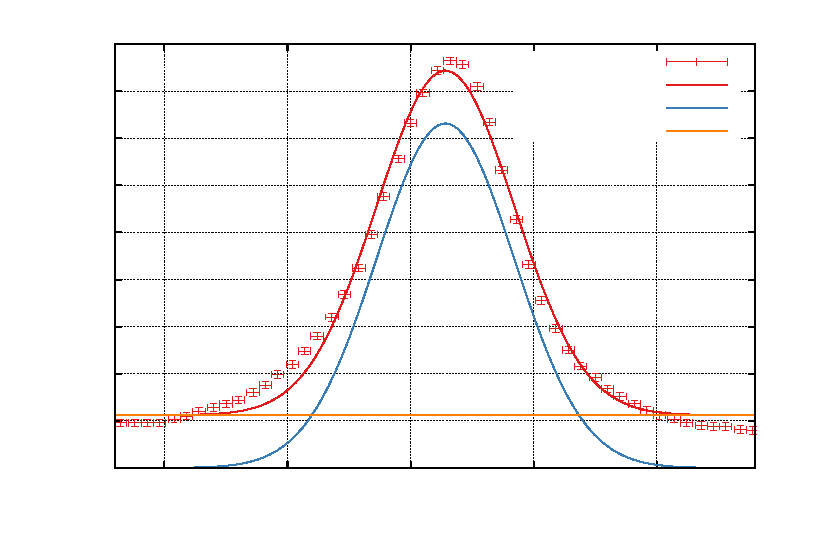
\includegraphics{./plots/b0}}%
    \gplfronttext
  \end{picture}%
\endgroup

	\caption{Intensitätsverteilung eines inneren Rings bei abgeschaltetem Magnetfeld zur Bestimmung des Auflösungsvermögens über die Halbwertsbreite des Maximums.}
	\label{fig:gauss0}
\end{figure}
Die Anpassung der Gaußfunktion liefert für den Peakschwerpunkt $\alpha$ und die Standardabweichung $\sigma$:
\begin{align*}
	\alpha &= \SI{1.01413 +- 0.00045}{\degree}\\
	\sigma &= \SI{0.02800 +- 0.00054}{\degree}
\end{align*}
Man sieht, dass die Anpassung nicht gut ist ($\chi^2_\mathrm{d.o.f.} = 9.8$), da die Kurve maßgeblich von der Gaußform abweicht.
Dennoch sollte die somit ermittelbare Halbwertsbreite für eine Abschätzung des Auflösungsvermögens ausreichend sein.
Die Halbwertsbreite $\mathrm{HBW}$ der Gaußfunktion mit Standardabweichung $\sigma$ berechnet sich aus:
\begin{align*}
\mathrm{HWB} &= 2 \sqrt{2\log(2)} \cdot \sigma\\
 &= \SI{0.0659 +- 0.0013}{\degree}
\end{align*}
Um diese in die Halbwertsbreite in Einheiten der Wellenlänge $\delta \lambda$ umzurechnen, verwenden wir die lineare Näherung aus der Interferenzbedingung des Etalons:
\begin{align*}
	\delta \lambda &= \left| \frac{\mathrm{d}\lambda}{\mathrm{d}\alpha} \right| \cdot \mathrm{HWB} \\
	 &= \frac{2d}{m} \, \frac{\sin(\alpha) \cos(\alpha)}{\sqrt{n^2-\sin^2(\alpha)}} \cdot \mathrm{HWB}\text{,}
\end{align*}
womit wir eine Linienbreite von:
\begin{align*}
	\delta \lambda = \SI{6.18 +- 0.13}{\pico\metre}
\end{align*}
erhalten.
Dabei wurde der Fehler über Gaußsche Fehlerfortpflanzung unter Beachtung der Fehler für die Halbwertsbreite $\mathrm{HWB}$ und den Peakschwerpunkt $\alpha$ beachtet.
Wie zuvor kann nun das Auflösungsvermögen und daraus die Finesse berechnet werden:
\begin{align}
	\mathcal{R} &= \frac{\lambda}{\delta \lambda} = \num{104200 +- 2200} \\
	\mathcal{F} &= \frac{\mathcal{R}}{m} = \num{5.76 +- 0.13}\text{.}
\end{align}
Die Bestimmung mit der CCD-Kamera war nicht erfolgreich, da die berechneten Werte für Auflösungsvermögen und Finesse etwa um einen Faktor $2$ von den Theoretischen abweichen.
Auf die möglichen Ursachen soll im Abschnitt \ref{ssec:diskussion_zeeman} eingegangen werden.

\noindent
\textbf{Dopper-Verbreiterung der Linie:}
Die Halbwertsbreite der gaußförmigen Doppler-Verbreiterung ist gegeben mit Gleichung (HIER REFERENZ) aus dem Grundlagenteil.
Bei der Temperatur $T = \SI{1000}{\K}$ folgt mit der Atommasse von Cadmium\footnote{CIAAW: 2013 Standard Atomic Weights\\http://www.ciaaw.org/atomic-weights.htm\\Letzer Aufruf: 26. November 2014} $m_\mathrm{Cd} = \SI{112.414 +- 0.004}{\atomicmassunit} $ die Doppler-Verbreiterung:
\begin{align}
	\delta \lambda_\mathrm{Doppler} = \SI{1.38}{\pico\metre}
\end{align}
Somit liegt die Doppler-Verbreiterung in derselben Größenordnung wie die mit der CCD-Kamera gemessene Breite von $\delta \lambda = \SI{6.18 +- 0.13}{\pico\metre}$.
Dennoch ist die Verbreiterung aufgrund des Doppler-Effekts von untergeordneter Bedeutung, da diese etwa einen Faktor \num{4.5} kleiner ist, als die tatsächlich beobachtete Breite.

\subsection{Diskussion}
\label{ssec:diskussion_zeeman}
Hier die Fehler mit der CCD-Kamera erklären!!!

% damit ich nicht wahnsinnig werde
\FloatBarrier

\section{Franck-Hertz-Versuch}

Wir wollen mit dem Franck-Hertz-Versuch den gequantelten Energieübertrag bei Stößen zwischen Elektronen und Quecksilberatomen beobachten und aus den Messwerten die Anregungsenergie von Quecksilber bestimmen.
Dabei soll die Temperatur- und Gegenspannungsabhängigkeit des zu messenden Anodenstroms beobachtet werden.

\subsection{Durchführung}

Der Versuch war bereits  wie in Abbildung \ref{fig:franck-hertz_aufbau} dargestellt aufgebaut, so dass lediglich das Cassy-Instrument in Betrieb genommen werden musste.
Dieses misst einmal die vom Steuergerät der Röhre ausgegebene Beschleunigungsspannung und digitalisiert die am anderen Ausgang liegende Spannung, die intern über einen Widerstand aus dem Anodenstrom gewonnen wird.
Da $U=R\,I$ gilt und konkrete Werte des Anodenstroms für die Auswertung irrelevant sind, braucht diese Umwandlung nicht weiter berücksichtigt werden.

An dem Gerät, das mit dem Ofen verbunden ist, können diverse Parameter eingestellt werden, unter anderem die für uns relevante Signalform der Beschleunigungsspannung (wir wählen gemäß der Anleitung eine positive Rampe), sowie deren Maximalwert und die Temperatur der Röhre.
Diese stellen wir auf \SI{160}{\degreeCelsius} ein, bei der das Quecksilber im geforderten Zwei-Phasen-System (am Phasenübergang zwischen gasförmig und flüssig) vorliegt.
Weiterhin können Temperatur der Röhre eingestellt und aktuelle Temperaturwerte überprüft werden, sowie einige weitere Optionen, die für den Versuch nicht benötigt wurden.
Vor jeder Messung haben wir mit der Option, manuell die Beschleunigungsspannung einzustellen, diese langsam erhöht bis der Effekt des Durchzündens erkennbar war und haben für den Maximalwert der Beschleunigungsspannung einen leicht darunter liegenden Wert gewählt, um den Aufbau nicht zu beschädigen.
Wir nutzen in der Auswertung die Bezeichnungen, wie sie auch in Abbildung \ref{fig:franck-hertz_aufbau} verwendet wurden.

\subsection{Messdaten}

Zunächst führen wir die Messung für verschiedene Gegenspannungen bei konstanter Temperatur durch.
Für diese wählen wir \SI{160}{\degreeCelsius} und überprüfen vor den Messungen, wie oben angesprochen, dass kein Durchzünden stattfinden kann.
Darum wählen wir als Maximalwert der positiven Rampe \SI{42}{\volt} und messen für vier Gegenspannungen zwischen \SI{2}{\volt} und \SI{3.5}{\volt} den Anodenstrom.
Die Messwerte sind in Abbildung \ref{fig:fh_varvolt} dargestellt.
Für die Diagramme wählen wir zur Skalierung der $y$-Achse willkürliche Einheiten, da diese nicht zur Auswertung benötigt werden und durch die im Steuergerät durchgeführte Umwandlung des Stroms in eine von Cassy messbare Spannung der Umrechnungsfaktor nicht bekannt ist.
Die geschätzten Fehler von \SI{0.1}{\volt} für die Beschleunigungsspannung und \num{0.1} willkürliche Einheiten für den Anodenstrom (in gleicher Skalierung wie die Werte von $I$) sind in dieser Darstellung sehr klein und wurden aus Gründen der Übersichtlichkeit nicht dargestellt.
\begin{figure}[!h]
\centering
% GNUPLOT: LaTeX picture with Postscript
\begingroup
  \makeatletter
  \providecommand\color[2][]{%
    \GenericError{(gnuplot) \space\space\space\@spaces}{%
      Package color not loaded in conjunction with
      terminal option `colourtext'%
    }{See the gnuplot documentation for explanation.%
    }{Either use 'blacktext' in gnuplot or load the package
      color.sty in LaTeX.}%
    \renewcommand\color[2][]{}%
  }%
  \providecommand\includegraphics[2][]{%
    \GenericError{(gnuplot) \space\space\space\@spaces}{%
      Package graphicx or graphics not loaded%
    }{See the gnuplot documentation for explanation.%
    }{The gnuplot epslatex terminal needs graphicx.sty or graphics.sty.}%
    \renewcommand\includegraphics[2][]{}%
  }%
  \providecommand\rotatebox[2]{#2}%
  \@ifundefined{ifGPcolor}{%
    \newif\ifGPcolor
    \GPcolortrue
  }{}%
  \@ifundefined{ifGPblacktext}{%
    \newif\ifGPblacktext
    \GPblacktexttrue
  }{}%
  % define a \g@addto@macro without @ in the name:
  \let\gplgaddtomacro\g@addto@macro
  % define empty templates for all commands taking text:
  \gdef\gplbacktext{}%
  \gdef\gplfronttext{}%
  \makeatother
  \ifGPblacktext
    % no textcolor at all
    \def\colorrgb#1{}%
    \def\colorgray#1{}%
  \else
    % gray or color?
    \ifGPcolor
      \def\colorrgb#1{\color[rgb]{#1}}%
      \def\colorgray#1{\color[gray]{#1}}%
      \expandafter\def\csname LTw\endcsname{\color{white}}%
      \expandafter\def\csname LTb\endcsname{\color{black}}%
      \expandafter\def\csname LTa\endcsname{\color{black}}%
      \expandafter\def\csname LT0\endcsname{\color[rgb]{1,0,0}}%
      \expandafter\def\csname LT1\endcsname{\color[rgb]{0,1,0}}%
      \expandafter\def\csname LT2\endcsname{\color[rgb]{0,0,1}}%
      \expandafter\def\csname LT3\endcsname{\color[rgb]{1,0,1}}%
      \expandafter\def\csname LT4\endcsname{\color[rgb]{0,1,1}}%
      \expandafter\def\csname LT5\endcsname{\color[rgb]{1,1,0}}%
      \expandafter\def\csname LT6\endcsname{\color[rgb]{0,0,0}}%
      \expandafter\def\csname LT7\endcsname{\color[rgb]{1,0.3,0}}%
      \expandafter\def\csname LT8\endcsname{\color[rgb]{0.5,0.5,0.5}}%
    \else
      % gray
      \def\colorrgb#1{\color{black}}%
      \def\colorgray#1{\color[gray]{#1}}%
      \expandafter\def\csname LTw\endcsname{\color{white}}%
      \expandafter\def\csname LTb\endcsname{\color{black}}%
      \expandafter\def\csname LTa\endcsname{\color{black}}%
      \expandafter\def\csname LT0\endcsname{\color{black}}%
      \expandafter\def\csname LT1\endcsname{\color{black}}%
      \expandafter\def\csname LT2\endcsname{\color{black}}%
      \expandafter\def\csname LT3\endcsname{\color{black}}%
      \expandafter\def\csname LT4\endcsname{\color{black}}%
      \expandafter\def\csname LT5\endcsname{\color{black}}%
      \expandafter\def\csname LT6\endcsname{\color{black}}%
      \expandafter\def\csname LT7\endcsname{\color{black}}%
      \expandafter\def\csname LT8\endcsname{\color{black}}%
    \fi
  \fi
  \setlength{\unitlength}{0.0500bp}%
  \begin{picture}(7200.00,5760.00)%
    \gplgaddtomacro\gplbacktext{%
      \csname LTb\endcsname%
      \put(814,704){\makebox(0,0)[r]{\strut{} 0}}%
      \csname LTb\endcsname%
      \put(814,1662){\makebox(0,0)[r]{\strut{} 2}}%
      \csname LTb\endcsname%
      \put(814,2620){\makebox(0,0)[r]{\strut{} 4}}%
      \csname LTb\endcsname%
      \put(814,3579){\makebox(0,0)[r]{\strut{} 6}}%
      \csname LTb\endcsname%
      \put(814,4537){\makebox(0,0)[r]{\strut{} 8}}%
      \csname LTb\endcsname%
      \put(814,5495){\makebox(0,0)[r]{\strut{} 10}}%
      \csname LTb\endcsname%
      \put(946,484){\makebox(0,0){\strut{} 0}}%
      \csname LTb\endcsname%
      \put(1678,484){\makebox(0,0){\strut{} 5}}%
      \csname LTb\endcsname%
      \put(2410,484){\makebox(0,0){\strut{} 10}}%
      \csname LTb\endcsname%
      \put(3142,484){\makebox(0,0){\strut{} 15}}%
      \csname LTb\endcsname%
      \put(3875,484){\makebox(0,0){\strut{} 20}}%
      \csname LTb\endcsname%
      \put(4607,484){\makebox(0,0){\strut{} 25}}%
      \csname LTb\endcsname%
      \put(5339,484){\makebox(0,0){\strut{} 30}}%
      \csname LTb\endcsname%
      \put(6071,484){\makebox(0,0){\strut{} 35}}%
      \csname LTb\endcsname%
      \put(6803,484){\makebox(0,0){\strut{} 40}}%
      \put(176,3099){\rotatebox{-270}{\makebox(0,0){\strut{}Anodenstrom $I$ / w.E.}}}%
      \put(3874,154){\makebox(0,0){\strut{}Beschleunigungsspannung $U$ / \si{\kilo\volt}}}%
      \put(3874,5385){\makebox(0,0){\strut{}}}%
    }%
    \gplgaddtomacro\gplfronttext{%
      \csname LTb\endcsname%
      \put(2266,5322){\makebox(0,0)[r]{\strut{}$\Delta U=\SI{2.0}{\volt}$}}%
      \csname LTb\endcsname%
      \put(2266,5102){\makebox(0,0)[r]{\strut{}$\Delta U=\SI{2.5}{\volt}$}}%
      \csname LTb\endcsname%
      \put(2266,4882){\makebox(0,0)[r]{\strut{}$\Delta U=\SI{3.0}{\volt}$}}%
      \csname LTb\endcsname%
      \put(2266,4662){\makebox(0,0)[r]{\strut{}$\Delta U=\SI{3.5}{\volt}$}}%
    }%
    \gplbacktext
    \put(0,0){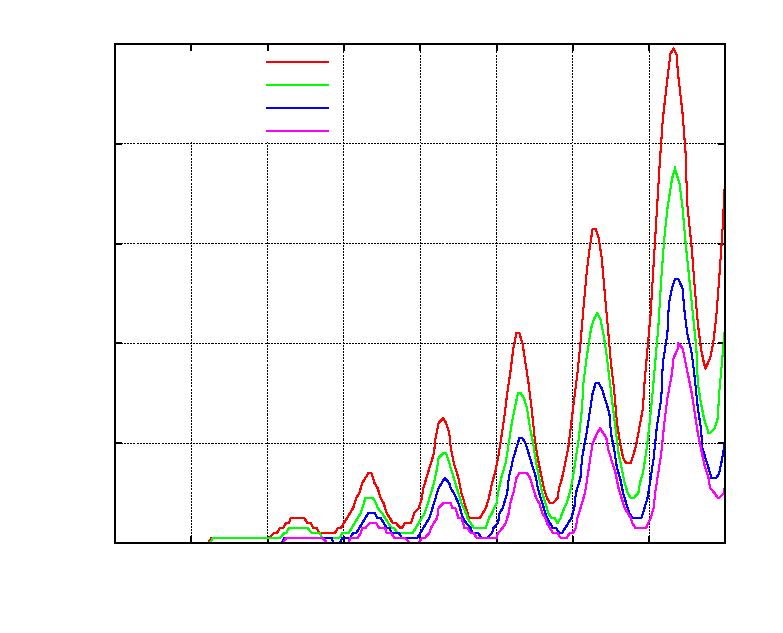
\includegraphics{./plots/fh_varvolt}}%
    \gplfronttext
  \end{picture}%
\endgroup

\caption{Variable Gegenspannung bei $T=\SI{160}{\degreeCelsius}$}
\label{fig:fh_varvolt}
\end{figure}
Für die Messung mit variabler Temperatur erhalten wir die in Abbildung \ref{fig:fh_vartemp} dargestellten Ergebnisse.
Dabei wählten wir als konstante Gegenspannung \SI{2}{\volt} und nutzen abermals willkürliche Einheiten für den gemessenen Anodenstrom.
\begin{figure}[!h]
\centering
% GNUPLOT: LaTeX picture with Postscript
\begingroup
  \makeatletter
  \providecommand\color[2][]{%
    \GenericError{(gnuplot) \space\space\space\@spaces}{%
      Package color not loaded in conjunction with
      terminal option `colourtext'%
    }{See the gnuplot documentation for explanation.%
    }{Either use 'blacktext' in gnuplot or load the package
      color.sty in LaTeX.}%
    \renewcommand\color[2][]{}%
  }%
  \providecommand\includegraphics[2][]{%
    \GenericError{(gnuplot) \space\space\space\@spaces}{%
      Package graphicx or graphics not loaded%
    }{See the gnuplot documentation for explanation.%
    }{The gnuplot epslatex terminal needs graphicx.sty or graphics.sty.}%
    \renewcommand\includegraphics[2][]{}%
  }%
  \providecommand\rotatebox[2]{#2}%
  \@ifundefined{ifGPcolor}{%
    \newif\ifGPcolor
    \GPcolortrue
  }{}%
  \@ifundefined{ifGPblacktext}{%
    \newif\ifGPblacktext
    \GPblacktexttrue
  }{}%
  % define a \g@addto@macro without @ in the name:
  \let\gplgaddtomacro\g@addto@macro
  % define empty templates for all commands taking text:
  \gdef\gplbacktext{}%
  \gdef\gplfronttext{}%
  \makeatother
  \ifGPblacktext
    % no textcolor at all
    \def\colorrgb#1{}%
    \def\colorgray#1{}%
  \else
    % gray or color?
    \ifGPcolor
      \def\colorrgb#1{\color[rgb]{#1}}%
      \def\colorgray#1{\color[gray]{#1}}%
      \expandafter\def\csname LTw\endcsname{\color{white}}%
      \expandafter\def\csname LTb\endcsname{\color{black}}%
      \expandafter\def\csname LTa\endcsname{\color{black}}%
      \expandafter\def\csname LT0\endcsname{\color[rgb]{1,0,0}}%
      \expandafter\def\csname LT1\endcsname{\color[rgb]{0,1,0}}%
      \expandafter\def\csname LT2\endcsname{\color[rgb]{0,0,1}}%
      \expandafter\def\csname LT3\endcsname{\color[rgb]{1,0,1}}%
      \expandafter\def\csname LT4\endcsname{\color[rgb]{0,1,1}}%
      \expandafter\def\csname LT5\endcsname{\color[rgb]{1,1,0}}%
      \expandafter\def\csname LT6\endcsname{\color[rgb]{0,0,0}}%
      \expandafter\def\csname LT7\endcsname{\color[rgb]{1,0.3,0}}%
      \expandafter\def\csname LT8\endcsname{\color[rgb]{0.5,0.5,0.5}}%
    \else
      % gray
      \def\colorrgb#1{\color{black}}%
      \def\colorgray#1{\color[gray]{#1}}%
      \expandafter\def\csname LTw\endcsname{\color{white}}%
      \expandafter\def\csname LTb\endcsname{\color{black}}%
      \expandafter\def\csname LTa\endcsname{\color{black}}%
      \expandafter\def\csname LT0\endcsname{\color{black}}%
      \expandafter\def\csname LT1\endcsname{\color{black}}%
      \expandafter\def\csname LT2\endcsname{\color{black}}%
      \expandafter\def\csname LT3\endcsname{\color{black}}%
      \expandafter\def\csname LT4\endcsname{\color{black}}%
      \expandafter\def\csname LT5\endcsname{\color{black}}%
      \expandafter\def\csname LT6\endcsname{\color{black}}%
      \expandafter\def\csname LT7\endcsname{\color{black}}%
      \expandafter\def\csname LT8\endcsname{\color{black}}%
    \fi
  \fi
  \setlength{\unitlength}{0.0500bp}%
  \begin{picture}(7200.00,5760.00)%
    \gplgaddtomacro\gplbacktext{%
      \csname LTb\endcsname%
      \put(814,704){\makebox(0,0)[r]{\strut{} 0}}%
      \csname LTb\endcsname%
      \put(814,1662){\makebox(0,0)[r]{\strut{} 2}}%
      \csname LTb\endcsname%
      \put(814,2620){\makebox(0,0)[r]{\strut{} 4}}%
      \csname LTb\endcsname%
      \put(814,3579){\makebox(0,0)[r]{\strut{} 6}}%
      \csname LTb\endcsname%
      \put(814,4537){\makebox(0,0)[r]{\strut{} 8}}%
      \csname LTb\endcsname%
      \put(814,5495){\makebox(0,0)[r]{\strut{} 10}}%
      \csname LTb\endcsname%
      \put(946,484){\makebox(0,0){\strut{} 0}}%
      \csname LTb\endcsname%
      \put(1678,484){\makebox(0,0){\strut{} 5}}%
      \csname LTb\endcsname%
      \put(2410,484){\makebox(0,0){\strut{} 10}}%
      \csname LTb\endcsname%
      \put(3142,484){\makebox(0,0){\strut{} 15}}%
      \csname LTb\endcsname%
      \put(3875,484){\makebox(0,0){\strut{} 20}}%
      \csname LTb\endcsname%
      \put(4607,484){\makebox(0,0){\strut{} 25}}%
      \csname LTb\endcsname%
      \put(5339,484){\makebox(0,0){\strut{} 30}}%
      \csname LTb\endcsname%
      \put(6071,484){\makebox(0,0){\strut{} 35}}%
      \csname LTb\endcsname%
      \put(6803,484){\makebox(0,0){\strut{} 40}}%
      \put(176,3099){\rotatebox{-270}{\makebox(0,0){\strut{}Anodenstrom $I$ / w.E.}}}%
      \put(3874,154){\makebox(0,0){\strut{}Beschleunigungsspannung $U$ / \si{\kilo\volt}}}%
      \put(3874,5385){\makebox(0,0){\strut{}}}%
    }%
    \gplgaddtomacro\gplfronttext{%
      \csname LTb\endcsname%
      \put(2134,5322){\makebox(0,0)[r]{\strut{} $T=\SI{155}{\degreeCelsius}$}}%
      \csname LTb\endcsname%
      \put(2134,5102){\makebox(0,0)[r]{\strut{} $T=\SI{160}{\degreeCelsius}$}}%
      \csname LTb\endcsname%
      \put(2134,4882){\makebox(0,0)[r]{\strut{} $T=\SI{165}{\degreeCelsius}$}}%
      \csname LTb\endcsname%
      \put(2134,4662){\makebox(0,0)[r]{\strut{} $T=\SI{170}{\degreeCelsius}$}}%
    }%
    \gplbacktext
    \put(0,0){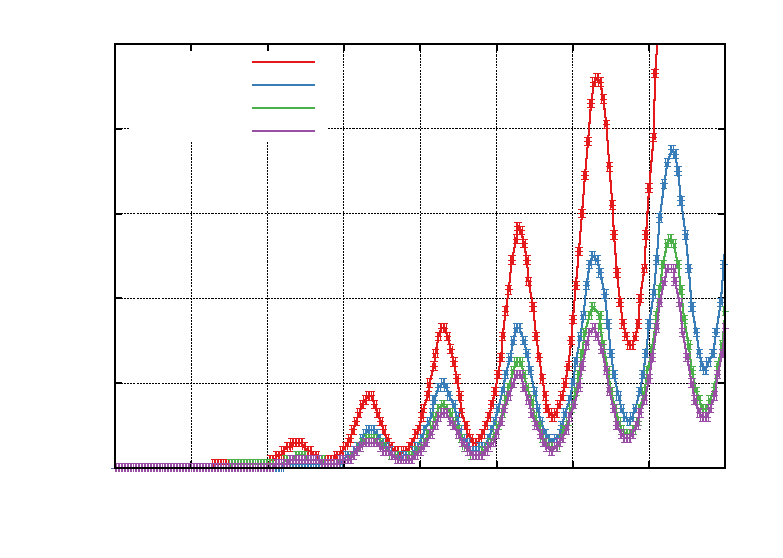
\includegraphics{./plots/fh_vartemp}}%
    \gplfronttext
  \end{picture}%
\endgroup

\caption{Variable Temperatur bei $\Delta U=\SI{2}{\volt}$ Gegenspannung}
\label{fig:fh_vartemp}
\end{figure}

\subsection{Auswertung}

\subsubsection{Energiedifferenz zwischen 6S- und 6P-Niveau in Quecksilber}

Zur Bestimmung der Energiedifferenz $\Delta E$ fitten wir mit gnuplot Gaußkurven an die Daten.
Als Fithypothese wählen wir dabei
\begin{align}
\mathcal{G}_i(x)=A\,\exp\left[-\frac{1}{2}\left(\frac{x-S_i}{\sigma_i}\right)^2\right] + c
\label{eq:fh_fithypothese}
\end{align}
mit dem Peakschwerpunkt $S_i$ und der Schwankungsbreite $\sigma_i$ , die wir beide zur Auswertung benötigen.
Wir lassen die Parameter nun an jeweils 4 Maxima pro Datensatz anpassen, wobei wir die Maxima mit $i$ von links nach rechts durchnummerieren, beginnend bei dem Maximum zwischen \SI{15}{\volt} und \SI{20}{\volt}, da das davor liegende besonders für hohe Gegenspannungen und hohe Temperaturen nicht gut angepasst werden kann.
Die Ergebnisse für die Schwerpunkte $S_i$ sind in Tabelle \ref{tab:fh_schwerpunkte} dargestellt.
Für den Fehler der zugrundeliegenden Messwerte schätzen wir \SI{0.1}{\volt} für die Beschleunigungsspannung und \num{0.1} für den Anodenstrom ab.
Zur Bestimmung des Energieabstands $\left(\Delta E\right)'$ berechnen wir die Differenz der Schwerpunkte $S_i-S_{i-1}$ und mitteln über diese Werte, die zusammen mit dem (über die Standardabweichung bestimmten) Fehler bereits in die Tabelle eingetragen sind.
Nun mitteln wir die so gefundenen Werte, um einen Gesamtwert für den Energieabstand $\Delta E$ zu erhalten.
Wir finden so:
\begin{align*}
\Delta E = \SI{4.922+-0.021}{\electronvolt}
\end{align*}
\begin{table}[h]
\centering
\resizebox{\columnwidth}{!}{%
\begin{tabular}{llllll}
\toprule
$\Delta$U / \si{\volt} & $S_1$ / \si{\kilo\volt} & $S_2$ / \si{\kilo\volt} & $S_3$ / \si{\kilo\volt} & $S_4$ / \si{\kilo\volt} & Mittelwert\\
\midrule
\num{2.0} &	\num{16.63+-0.02} & \num{21.45+-0.02} &	\num{26.42+-0.01} &	\num{31.44+-0.02} &	\num{4.94+-0.06}\\
\num{2.5} &	\num{16.77+-0.02} &	\num{21.59+-0.01} &	\num{26.58+-0.01} &	\num{31.61+-0.01} &	\num{4.95+-0.07}\\
\num{3.0} &	\num{16.92+-0.03} &	\num{21.68+-0.02} &	\num{26.71+-0.02} &	\num{31.74+-0.01} &	\num{4.94+-0.09}\\
\num{3.5} &	\num{16.99+-0.05} &	\num{21.83+-0.03} &	\num{26.84+-0.02} &	\num{31.90+-0.02} &	\num{4.97+-0.07}\\
	      &					  &			  	 	  &					  &					  &					\\
{T / \si{\degreeCelsius}} & & & & & \\
\midrule
\num{155} &	\num{16.61+-0.02} &	\num{21.52+-0.02} &	\num{26.51+-0.02} &	\num{31.63+-0.02} &	\num{5.01+-0.07}\\
\num{160} &	\num{16.81+-0.04} &	\num{21.51+-0.02} &	\num{26.43+-0.02} &	\num{31.43+-0.02} &	\num{4.87+-0.10}\\
\num{165} &	\num{16.82+-0.04} &	\num{21.55+-0.02} &	\num{26.42+-0.02} &	\num{31.36+-0.02} &	\num{4.85+-0.07}\\
\num{170} &	\num{16.82+-0.05} &	\num{21.60+-0.02} &	\num{26.40+-0.02} &	\num{31.36+-0.02} &	\num{4.85+-0.06}\\
\bottomrule
\end{tabular}}
\caption{Messwerte der Peakschwerpunkte für variable $\Delta U$ bei \SI{160}{\degreeCelsius} bzw. variable Temperatur bei $\Delta U=\SI{2}{\volt}$}
\label{tab:fh_schwerpunkte}
\end{table}
Um diesen Wert zu verstehen, muss man das Termschema (Abb. \ref{fig:termschema_hg}) und den Wirkungsquerschnitt bei Elektronenstoßanregung von Quecksilber (Abb. \ref{fig:wirkungsquerschnitt_hg}) betrachten.
\begin{figure}[h]
\centering
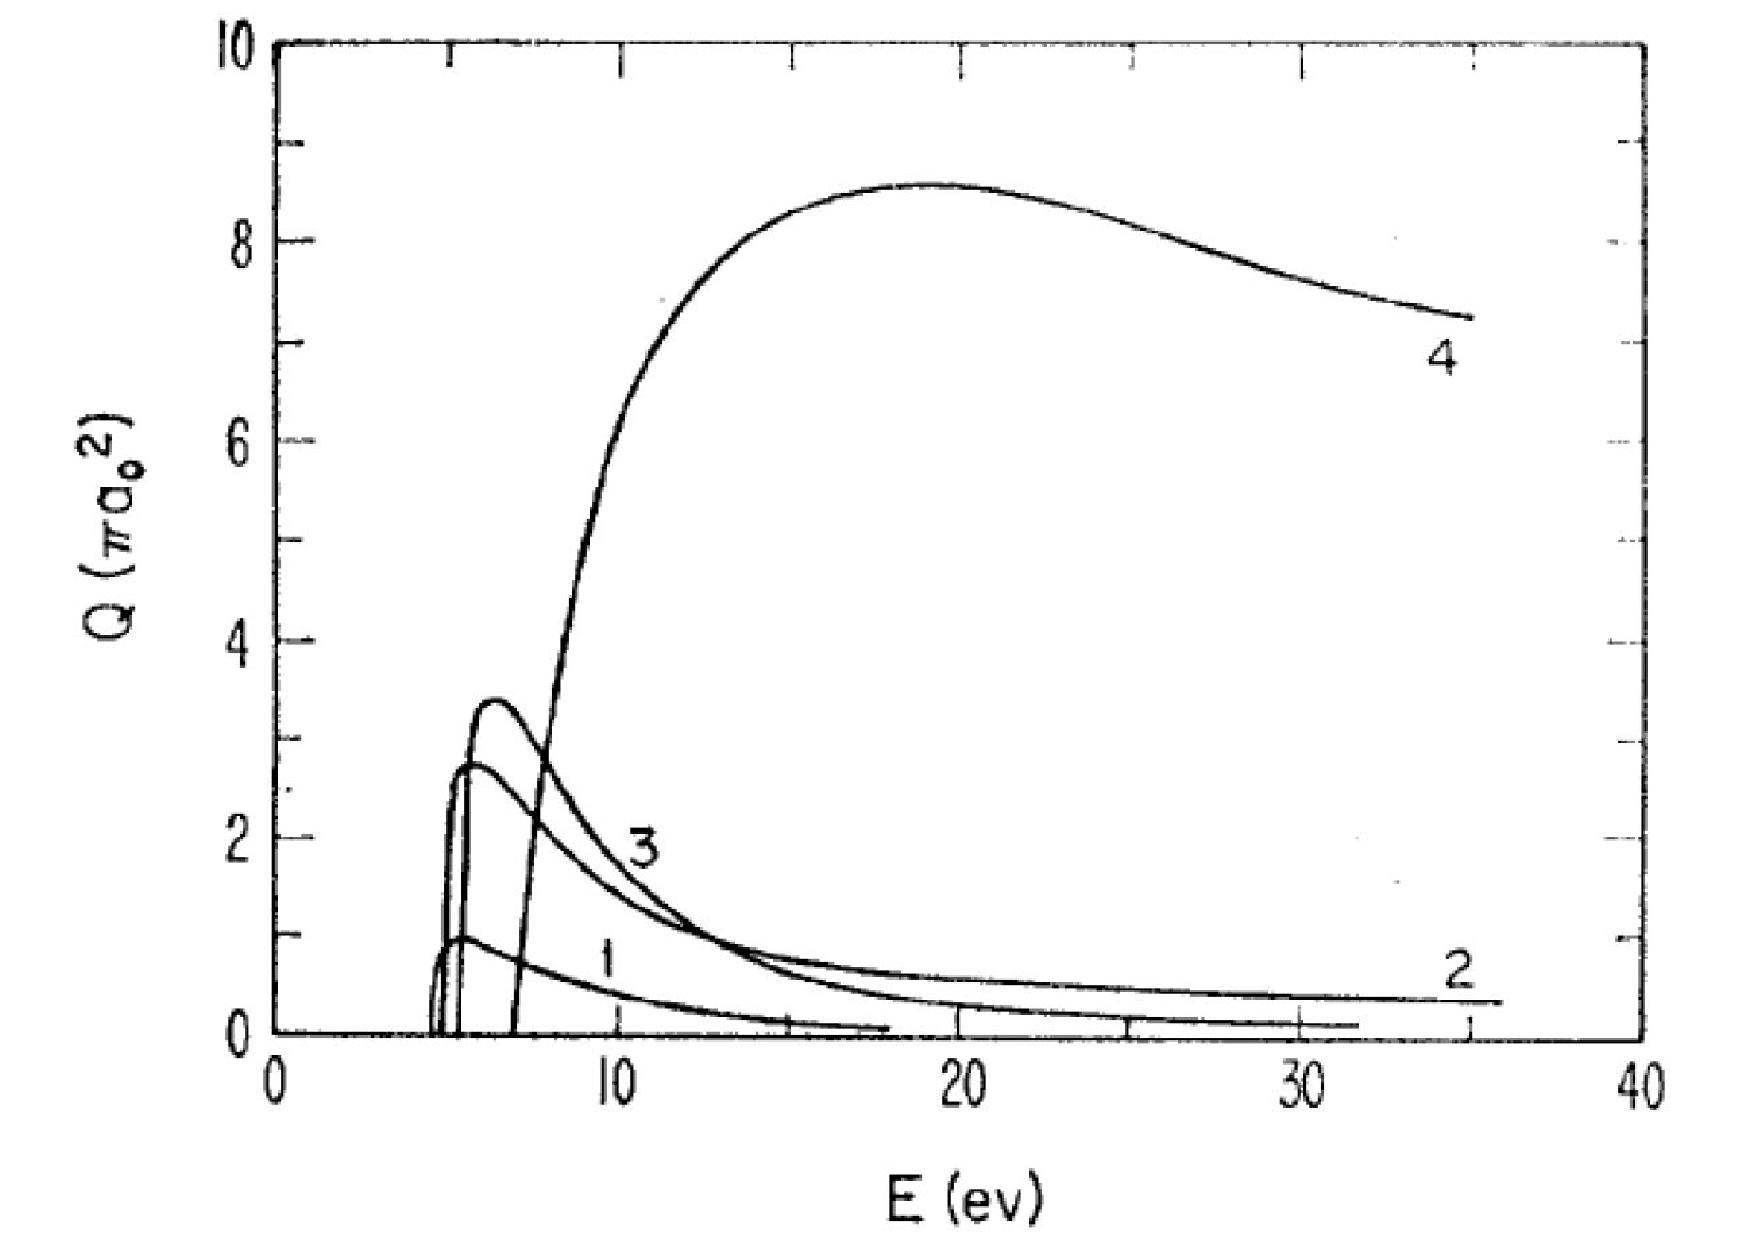
\includegraphics[width=0.6\textwidth]{./figures/wirkungsquerschnitt_hg.pdf}
\caption{Totaler Wirkungsquerschnitt von Quecksilber bei Elektronenstoßanregung. Die Linien entsprechen \textbf{1}: 6$^1$S$_0 \rightarrow$ 6$^3$P$_0$; \textbf{2}: 6$^1$S$_0 \rightarrow$ 6$^3$P$_1$; \textbf{3}: 6$^1$S$_0 \rightarrow$ 6$^3$P$_2$; \textbf{4}: 6$^1$S$_0 \rightarrow$ 6$^1$P$_1$. Quelle: Moiseiwitsch,
"`Electron Impact Excitation of Atoms"', Rev. Mod. Phys. 40, S. 267, 1968}
\label{fig:wirkungsquerschnitt_hg}
\end{figure}
In der Grafik zu letzterem sieht man vier Wirkungsquerschnitte für verschiedene Übergänge im Quecksilber in Abhängigkeit von den stoßenden Elektronen.
Da Linie 4 erst knapp unter \SI{20}{\electronvolt} ihr Maximum hat, Stöße offensichtlich aber auch schon bei geringen Energien stattfinden, werden wir diese nicht weiter beachten.
Genauso ignorieren wir Linie 1, da der maximale Wirkungsquerschnitt hier sehr gering ist im Vergleich zu den anderen in Betracht kommenden Linien 2 und 3.

Wir betrachten zur weiteren Auswertung darum nur noch die Linien 2 und 3, wobei wir davon ausgehen können, dass der Wirkungsquerschnitt von Linie 2 ausreicht, um Stöße der Elektronen mit den Quecksilberatomen auszulösen.
Ein Argument für diese Annahme ist, dass die Linie bei geringeren Energien als Linie 3 sowohl beginnt, als auch ihr Maximum erreicht.
Die Linie 2 korrespondiert mit dem Übergang $6^1$S$_0\rightarrow6^3$P$_1$, so dass dieser am häufigsten stattfinden wird.
Dennoch können einige Elektronen bei dieser Energie keine Stöße ausführen und werden weiter beschleunigt, so dass diese gemäß Linie 3 stoßen werden.
Darum wird der Übergang $6^1$S$_0\rightarrow6^3$P$_2$ in den Messwerten auch zu finden sein.

Zusammen mit dem Termschema, mit dem der Linie 2 die Energie \SI{4.89}{\electronvolt} und Linie 3 die Energie \SI{5.46}{\electronvolt} zugeordnet werden kann, erklärt sich damit die gefundene Energiedifferenz von $\Delta E = \SI{4.922+-0.021}{\electronvolt}$.
Diese liegt knapp über dem Wert von \SI{4.89}{\electronvolt}, da nebem diesem Übergang in Quecksilber auch einer mit \SI{5.46}{\electronvolt} stattfindet, allerdings deutlich seltener.

\begin{table}[h]
\centering
\begin{tabular}{lllll}
\toprule
$\Delta$U / \si{\volt} & $\sigma_1$ / \si{\volt} & $\sigma_2$ / \si{\volt} & $\sigma_3$ / \si{\volt} & $\sigma_4$ / \si{\volt} \\
\midrule
\num{2,0}	& \num{0.79+-0.03} &	\num{0.80+-0.03} &	\num{0.87+-0.02} &	\num{0.91+-0.03}	\\
\num{2.5}	& \num{0.73+-0.04} &	\num{0.77+-0.02} &	\num{0.84+-0.02} &	\num{0.92+-0.02}	\\
\num{3,0}	& \num{0.74+-0.05} &	\num{0.74+-0.03} &	\num{0.82+-0.03} &	\num{0.90+-0.03}	\\
\num{3.5}	& \num{0.73+-0.07} &	\num{0.73+-0.02} &	\num{0.77+-0.03} &	\num{0.87+-0.04}	\\
	      &					  &			  	 	  &					  &			\\
T / \si{\degreeCelsius} & & & & \\
\midrule
\num{155}	& \num{0.79+-0.02} &	\num{0.83+-0.02} &	\num{0.92+-0.02} &	\num{1.00+-0.03}	\\
\num{160}	& \num{0.84+-0.05} &	\num{0.78+-0.03} &	\num{0.87+-0.02} &	\num{0.89+-0.03}	\\
\num{165}	& \num{0.83+-0.05} &	\num{0.80+-0.02} &	\num{0.84+-0.03} &	\num{0.83+-0.03}	\\
\num{170}	& \num{0.87+-0.06} &	\num{0.83+-0.03} &	\num{0.83+-0.03} &	\num{0.86+-0.03} 	\\
\bottomrule
\end{tabular}
\caption{Messwerte der Schwankungsbreite für variable $\Delta U$ bei \SI{160}{\degreeCelsius} bzw. variable Temperatur bei $\Delta U=\SI{2}{\volt}$}
\label{tab:fh_breite}
\end{table}
Ferner sind in Tabelle \ref{tab:fh_breite} für jede Kurve die Schwankungsbreiten dargestellt, die bestimmt werden sollen.
Wir lesen sie direkt aus den von gnuplot angepassten Parametern an unsere Fithypothese (\ref{eq:fh_fithypothese}) ab.
Dabei fällt auf, dass die Breite der Kurven für die Messwerte bei konstanter Temperatur, sowie bei den Temperaturen \SI{155}{\degreeCelsius} und \SI{160}{\degreeCelsius}, mit steigender Beschleunigungsspannung zunimmt.
Für die beiden höchsten Temperaturen ist keine eindeutige Änderung der Schwankungsbreite erkennbar.

\subsubsection{Abhängigkeit des Anodenstroms von der Gegenspannung}

Zur Abhängigkeit des Anodenstroms von der Röhrentemperatur bzw. der angelegten Gegenspannung zwischen Gitter und Anode betrachten wir zunächst die Abbildung \ref{fig:fh_varvolt}, bei der die Temperatur für alle Messungen \SI{160}{\degreeCelsius} betrug.
Man sieht in dieser Darstellungsform deutlich, dass die Maxima für höhere Gegenspannungen kleiner werden, was daran liegt, dass die Elektronen nach dem Stoß nicht mehr genügend Energie haben, um die Gegenspannung zu durchlaufen.
Sie werden demzufolge nicht an der Anode registriert und der Anodenstrom sinkt im Vergleich zu einer geringeren Gegenspannung.
Weiterhin fällt auf, dass die Minima für höhere Gegenspannungen ebenfalls niedriger liegen.
Die Ursache dafür liegt an Elektronen geringer Energien nach dem Stoß, beispielsweise \SI{2.5}{\electronvolt}.
Ein Elektron dieser Energie kann bei \SI{2}{\volt} Gegenspannung noch registriert werden, bei \SI{3}{\volt} nicht mehr, weswegen der Anodenstrom im zweiten Fall kleiner ist.
Als letztes bemerkt man, dass sich die Extrema für höhere Gegenspannungen nach rechts verschieben, was sich mit dem Beschleunigungsprozess der Elektronen erklären lässt.
Diese müssen eine höhere Beschleunigungsspannung durchlaufen, um nach dem Stoß noch genügend Energie zu haben, damit sie die Anode erreichen.

\subsubsection{Abhängigkeit des Anodenstroms von der Temperatur}
Zur Abhängigkeit des Anodenstroms von der Temperatur schauen wir uns Abbildung \ref{fig:fh_vartemp} an, in der die Temperatur bei den Messungen variiert und die Gegenspannung konstant bei \SI{2}{\volt} gehalten wurde.
In dem Diagramm sind ebenfalls alle Messreihen gleichzeitig dargestellt, um optimal vergleichen zu können.
Man erkennt, dass der Anodenstrom für höhere Temperaturen kleiner ist als für niedrige Temperaturen, besonders die Kurve für $T=\SI{155}{\degreeCelsius}$ ist dabei deutlich höher und bei gleichen Temperaturabständen deutlich weiter entfernt von den anderen Messungen.
Wir benötigen die in der Praktikumsanleitung angegebene Formel zum Dampfdruck von Quecksilber zur Erklärung der Beobachtung:
\begin{align}
\log p = 10,55-3333/T-0,85\log T \quad \text{($p$ in Torr und $T$ in K)}
\label{eq:dampfdruck}
\end{align}
Man erkennt daran, dass der Dampfdruck mit der Temperatur steigt und somit bei höheren Temperaturen mehr gasförmige Quecksilberatome vorhanden sind.
Dies erhöht die Stoßwahrscheinlichkeit der Elektronen und es werden weniger gestoßene Elektronen die Gegenspannung durchlaufen und die Anode erreichen, weswegen der Strom sinkt.
Eine Verschiebung der Extrema wie bei der Abhängigkeit von der Gegenspannung ist für die Temperaturabhängigkeit des Anodenstroms nicht festzustellen.
\\
\\
Die starke Abweichung der Kurve für $T=\SI{155}{\degreeCelsius}$ kann dabei gleichzeitig mit der Frage beantwortet werden, warum die Durchführung des Franck-Hertz-Versuches mit Quecksilber auf ein kleines Temperaturintervall beschränkt ist.
Der Grund dafür ist das Zwei-Phasen-System in dem sich das Quecksilber befindet.
Dabei bewegt es sich ständig am Phasenübergang zwischen gasförmig und flüssig und ist dadurch nur auf einen schmalen Temperatur- bzw. Druckbereich begrenzt, wobei der Druck mit (\ref{eq:dampfdruck}) in Abhängigkeit von der Temperatur gegeben ist.
Bei zu hohen Temperaturen bzw. entsprechend zu hoher Teilchendichte steigt außerdem die Zündspannung der Röhre, was den Temperaturbereich nach oben hin begrenzt, da ein Durchzünden vermieden werden sollte. 
Um sinnvolle Messungen durchzuführen darf die Temperatur daher nur wenig um einen geeigneten Wert variiert werden und die Versuchsdurchführung ist auf ein kleines Temperaturintervall begrenzt, welches wir für $T=\SI{155}{\degreeCelsius}$ möglicherweise unterschritten haben und so einen vergleichsweise sehr hohen Anodenstrom gemessen haben.
\\
\\
Ferner ist zu erklären, wieso die Einbrüche des Anodenstroms nicht scharf sind.
Die Ursache dafür liegt an dem glühelektrischen Effekt und der Erzeugung der freien Elektronen.
Ihr Geschwindigkeitsprofil folgt der Maxwell-Boltzmann-Verteilung, weswegen Elektronen mit höherer Geschwindigkeit ($\widehat{=}$ höherer Energie) früher mit Quecksilberatomen stoßen können als Elektronen, die mit niedrigerer Geschwindigkeit aus der Kathode austreten.
Weiterhin stoßen die Elektronen nicht sobald sie eine bestimmte Schwellenenergie erreicht haben, sondern durchlaufen die Beschleunigungsspannung weiter, auch wenn sie bereits die theoretisch benötigte Energie für einen Stoß haben und stoßen erst später mit einem Quecksilberatom, weswegen die Einbrüche des Anodenstroms nicht scharf sind.
Dass der Anodenstrom nicht bei jedem Einbruch auf \SI{0}{\ampere} abfällt ist darin begründet, dass nicht alle Elektronen einen Stoßpartner finden und manche ohne zu stoßen die Anode erreichen. 

\subsection{Diskussion}

\FloatBarrier

% BIBLIOGRAPHIE

% Maximale Anzahl der Einträge in Klammer
% Zitieren mit \cite{lamport94}
\begin{thebibliography}{9}

\bibitem{hecht}
	Eugene Hecht,
	\emph{Optik}.
	Oldenbourg,
	5. Auflage
	
\bibitem{siegmann}
	Anthony E. Siegmann,
	\emph{Lasers}.
	University Science Books,
	1986
	
\bibitem{demtroeder3}
	Wolfgang Demtröder,
	\emph{Experimentalphysik 3}.
	Springer Verlag,
	3. Auflage

\bibitem{np_richardson}
 Nobelprize.org,
 \emph{"The Nobel Prize in Physics 1928"}.
 Nobel Media AB 2014. Web. 15\\
 (\url{http://www.nobelprize.org/nobel_prizes/physics/laureates/1928/richardson-lecture.pdf} abgerufen am 15.11.2014)
\end{thebibliography}

% APPENDIX
\begin{appendix}
\section{Darstellung der Aufspaltung beim Zeeman-Effekt}
\label{app:penis}

\begin{sidewaysfigure}[!h]
\begin{subfigure}[c]{0.5\textwidth}
\scalebox{0.75}{
	% GNUPLOT: LaTeX picture with Postscript
\begingroup
  \makeatletter
  \providecommand\color[2][]{%
    \GenericError{(gnuplot) \space\space\space\@spaces}{%
      Package color not loaded in conjunction with
      terminal option `colourtext'%
    }{See the gnuplot documentation for explanation.%
    }{Either use 'blacktext' in gnuplot or load the package
      color.sty in LaTeX.}%
    \renewcommand\color[2][]{}%
  }%
  \providecommand\includegraphics[2][]{%
    \GenericError{(gnuplot) \space\space\space\@spaces}{%
      Package graphicx or graphics not loaded%
    }{See the gnuplot documentation for explanation.%
    }{The gnuplot epslatex terminal needs graphicx.sty or graphics.sty.}%
    \renewcommand\includegraphics[2][]{}%
  }%
  \providecommand\rotatebox[2]{#2}%
  \@ifundefined{ifGPcolor}{%
    \newif\ifGPcolor
    \GPcolortrue
  }{}%
  \@ifundefined{ifGPblacktext}{%
    \newif\ifGPblacktext
    \GPblacktexttrue
  }{}%
  % define a \g@addto@macro without @ in the name:
  \let\gplgaddtomacro\g@addto@macro
  % define empty templates for all commands taking text:
  \gdef\gplbacktext{}%
  \gdef\gplfronttext{}%
  \makeatother
  \ifGPblacktext
    % no textcolor at all
    \def\colorrgb#1{}%
    \def\colorgray#1{}%
  \else
    % gray or color?
    \ifGPcolor
      \def\colorrgb#1{\color[rgb]{#1}}%
      \def\colorgray#1{\color[gray]{#1}}%
      \expandafter\def\csname LTw\endcsname{\color{white}}%
      \expandafter\def\csname LTb\endcsname{\color{black}}%
      \expandafter\def\csname LTa\endcsname{\color{black}}%
      \expandafter\def\csname LT0\endcsname{\color[rgb]{1,0,0}}%
      \expandafter\def\csname LT1\endcsname{\color[rgb]{0,1,0}}%
      \expandafter\def\csname LT2\endcsname{\color[rgb]{0,0,1}}%
      \expandafter\def\csname LT3\endcsname{\color[rgb]{1,0,1}}%
      \expandafter\def\csname LT4\endcsname{\color[rgb]{0,1,1}}%
      \expandafter\def\csname LT5\endcsname{\color[rgb]{1,1,0}}%
      \expandafter\def\csname LT6\endcsname{\color[rgb]{0,0,0}}%
      \expandafter\def\csname LT7\endcsname{\color[rgb]{1,0.3,0}}%
      \expandafter\def\csname LT8\endcsname{\color[rgb]{0.5,0.5,0.5}}%
    \else
      % gray
      \def\colorrgb#1{\color{black}}%
      \def\colorgray#1{\color[gray]{#1}}%
      \expandafter\def\csname LTw\endcsname{\color{white}}%
      \expandafter\def\csname LTb\endcsname{\color{black}}%
      \expandafter\def\csname LTa\endcsname{\color{black}}%
      \expandafter\def\csname LT0\endcsname{\color{black}}%
      \expandafter\def\csname LT1\endcsname{\color{black}}%
      \expandafter\def\csname LT2\endcsname{\color{black}}%
      \expandafter\def\csname LT3\endcsname{\color{black}}%
      \expandafter\def\csname LT4\endcsname{\color{black}}%
      \expandafter\def\csname LT5\endcsname{\color{black}}%
      \expandafter\def\csname LT6\endcsname{\color{black}}%
      \expandafter\def\csname LT7\endcsname{\color{black}}%
      \expandafter\def\csname LT8\endcsname{\color{black}}%
    \fi
  \fi
  \setlength{\unitlength}{0.0500bp}%
  \begin{picture}(7486.00,5040.00)%
    \gplgaddtomacro\gplbacktext{%
      \csname LTb\endcsname%
      \put(814,704){\makebox(0,0)[r]{\strut{} 0}}%
      \csname LTb\endcsname%
      \put(814,1156){\makebox(0,0)[r]{\strut{} 5}}%
      \csname LTb\endcsname%
      \put(814,1609){\makebox(0,0)[r]{\strut{} 10}}%
      \csname LTb\endcsname%
      \put(814,2061){\makebox(0,0)[r]{\strut{} 15}}%
      \csname LTb\endcsname%
      \put(814,2513){\makebox(0,0)[r]{\strut{} 20}}%
      \csname LTb\endcsname%
      \put(814,2966){\makebox(0,0)[r]{\strut{} 25}}%
      \csname LTb\endcsname%
      \put(814,3418){\makebox(0,0)[r]{\strut{} 30}}%
      \csname LTb\endcsname%
      \put(814,3870){\makebox(0,0)[r]{\strut{} 35}}%
      \csname LTb\endcsname%
      \put(814,4323){\makebox(0,0)[r]{\strut{} 40}}%
      \csname LTb\endcsname%
      \put(814,4775){\makebox(0,0)[r]{\strut{} 45}}%
      \csname LTb\endcsname%
      \put(946,484){\makebox(0,0){\strut{} 0.8}}%
      \csname LTb\endcsname%
      \put(1714,484){\makebox(0,0){\strut{} 0.85}}%
      \csname LTb\endcsname%
      \put(2482,484){\makebox(0,0){\strut{} 0.9}}%
      \csname LTb\endcsname%
      \put(3250,484){\makebox(0,0){\strut{} 0.95}}%
      \csname LTb\endcsname%
      \put(4018,484){\makebox(0,0){\strut{} 1}}%
      \csname LTb\endcsname%
      \put(4785,484){\makebox(0,0){\strut{} 1.05}}%
      \csname LTb\endcsname%
      \put(5553,484){\makebox(0,0){\strut{} 1.1}}%
      \csname LTb\endcsname%
      \put(6321,484){\makebox(0,0){\strut{} 1.15}}%
      \csname LTb\endcsname%
      \put(7089,484){\makebox(0,0){\strut{} 1.2}}%
      \put(176,2739){\rotatebox{-270}{\makebox(0,0){\strut{}Intensität $I$ / \si{\percent}}}}%
      \put(4017,154){\makebox(0,0){\strut{}Winkel $\alpha$ / \si{\degree}}}%
      \put(4017,4665){\makebox(0,0){\strut{}}}%
    }%
    \gplgaddtomacro\gplfronttext{%
      \csname LTb\endcsname%
      \put(6102,4602){\makebox(0,0)[r]{\strut{}Messwerte}}%
      \csname LTb\endcsname%
      \put(6102,4382){\makebox(0,0)[r]{\strut{}Summe Gaußfits}}%
      \csname LTb\endcsname%
      \put(6102,4162){\makebox(0,0)[r]{\strut{}Funktion 1}}%
      \csname LTb\endcsname%
      \put(6102,3942){\makebox(0,0)[r]{\strut{}Funktion 2}}%
      \csname LTb\endcsname%
      \put(6102,3722){\makebox(0,0)[r]{\strut{}Funktion 3}}%
      \csname LTb\endcsname%
      \put(6102,3502){\makebox(0,0)[r]{\strut{}Untergrund}}%
    }%
    \gplbacktext
    \put(0,0){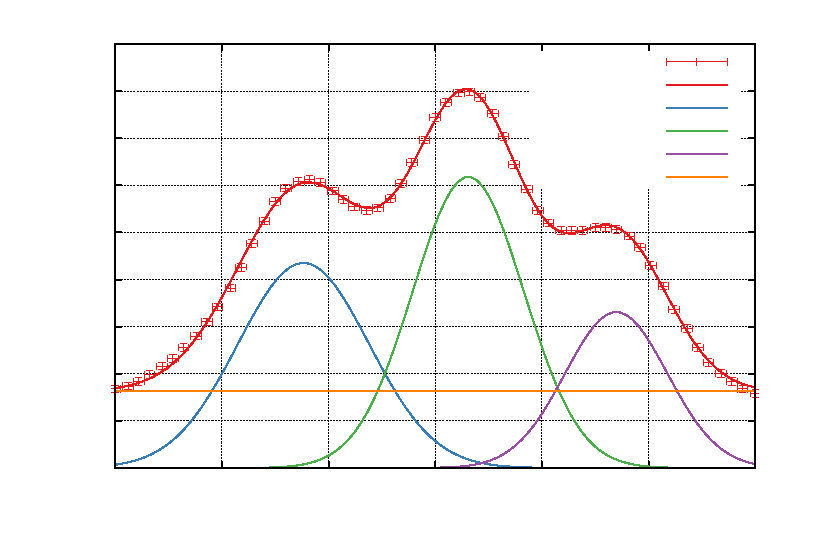
\includegraphics{./plots/zeemann_aufspaltung/b4}}%
    \gplfronttext
  \end{picture}%
\endgroup

	}
	\subcaption{}
\end{subfigure}
\begin{subfigure}[c]{0.5\textwidth}
\scalebox{0.75}{
	% GNUPLOT: LaTeX picture with Postscript
\begingroup
  \makeatletter
  \providecommand\color[2][]{%
    \GenericError{(gnuplot) \space\space\space\@spaces}{%
      Package color not loaded in conjunction with
      terminal option `colourtext'%
    }{See the gnuplot documentation for explanation.%
    }{Either use 'blacktext' in gnuplot or load the package
      color.sty in LaTeX.}%
    \renewcommand\color[2][]{}%
  }%
  \providecommand\includegraphics[2][]{%
    \GenericError{(gnuplot) \space\space\space\@spaces}{%
      Package graphicx or graphics not loaded%
    }{See the gnuplot documentation for explanation.%
    }{The gnuplot epslatex terminal needs graphicx.sty or graphics.sty.}%
    \renewcommand\includegraphics[2][]{}%
  }%
  \providecommand\rotatebox[2]{#2}%
  \@ifundefined{ifGPcolor}{%
    \newif\ifGPcolor
    \GPcolortrue
  }{}%
  \@ifundefined{ifGPblacktext}{%
    \newif\ifGPblacktext
    \GPblacktexttrue
  }{}%
  % define a \g@addto@macro without @ in the name:
  \let\gplgaddtomacro\g@addto@macro
  % define empty templates for all commands taking text:
  \gdef\gplbacktext{}%
  \gdef\gplfronttext{}%
  \makeatother
  \ifGPblacktext
    % no textcolor at all
    \def\colorrgb#1{}%
    \def\colorgray#1{}%
  \else
    % gray or color?
    \ifGPcolor
      \def\colorrgb#1{\color[rgb]{#1}}%
      \def\colorgray#1{\color[gray]{#1}}%
      \expandafter\def\csname LTw\endcsname{\color{white}}%
      \expandafter\def\csname LTb\endcsname{\color{black}}%
      \expandafter\def\csname LTa\endcsname{\color{black}}%
      \expandafter\def\csname LT0\endcsname{\color[rgb]{1,0,0}}%
      \expandafter\def\csname LT1\endcsname{\color[rgb]{0,1,0}}%
      \expandafter\def\csname LT2\endcsname{\color[rgb]{0,0,1}}%
      \expandafter\def\csname LT3\endcsname{\color[rgb]{1,0,1}}%
      \expandafter\def\csname LT4\endcsname{\color[rgb]{0,1,1}}%
      \expandafter\def\csname LT5\endcsname{\color[rgb]{1,1,0}}%
      \expandafter\def\csname LT6\endcsname{\color[rgb]{0,0,0}}%
      \expandafter\def\csname LT7\endcsname{\color[rgb]{1,0.3,0}}%
      \expandafter\def\csname LT8\endcsname{\color[rgb]{0.5,0.5,0.5}}%
    \else
      % gray
      \def\colorrgb#1{\color{black}}%
      \def\colorgray#1{\color[gray]{#1}}%
      \expandafter\def\csname LTw\endcsname{\color{white}}%
      \expandafter\def\csname LTb\endcsname{\color{black}}%
      \expandafter\def\csname LTa\endcsname{\color{black}}%
      \expandafter\def\csname LT0\endcsname{\color{black}}%
      \expandafter\def\csname LT1\endcsname{\color{black}}%
      \expandafter\def\csname LT2\endcsname{\color{black}}%
      \expandafter\def\csname LT3\endcsname{\color{black}}%
      \expandafter\def\csname LT4\endcsname{\color{black}}%
      \expandafter\def\csname LT5\endcsname{\color{black}}%
      \expandafter\def\csname LT6\endcsname{\color{black}}%
      \expandafter\def\csname LT7\endcsname{\color{black}}%
      \expandafter\def\csname LT8\endcsname{\color{black}}%
    \fi
  \fi
  \setlength{\unitlength}{0.0500bp}%
  \begin{picture}(7488.00,5040.00)%
    \gplgaddtomacro\gplbacktext{%
      \csname LTb\endcsname%
      \put(814,704){\makebox(0,0)[r]{\strut{} 0}}%
      \csname LTb\endcsname%
      \put(814,1156){\makebox(0,0)[r]{\strut{} 5}}%
      \csname LTb\endcsname%
      \put(814,1609){\makebox(0,0)[r]{\strut{} 10}}%
      \csname LTb\endcsname%
      \put(814,2061){\makebox(0,0)[r]{\strut{} 15}}%
      \csname LTb\endcsname%
      \put(814,2513){\makebox(0,0)[r]{\strut{} 20}}%
      \csname LTb\endcsname%
      \put(814,2966){\makebox(0,0)[r]{\strut{} 25}}%
      \csname LTb\endcsname%
      \put(814,3418){\makebox(0,0)[r]{\strut{} 30}}%
      \csname LTb\endcsname%
      \put(814,3870){\makebox(0,0)[r]{\strut{} 35}}%
      \csname LTb\endcsname%
      \put(814,4323){\makebox(0,0)[r]{\strut{} 40}}%
      \csname LTb\endcsname%
      \put(814,4775){\makebox(0,0)[r]{\strut{} 45}}%
      \csname LTb\endcsname%
      \put(1438,484){\makebox(0,0){\strut{} 0.9}}%
      \csname LTb\endcsname%
      \put(2667,484){\makebox(0,0){\strut{} 0.95}}%
      \csname LTb\endcsname%
      \put(3896,484){\makebox(0,0){\strut{} 1}}%
      \csname LTb\endcsname%
      \put(5125,484){\makebox(0,0){\strut{} 1.05}}%
      \csname LTb\endcsname%
      \put(6354,484){\makebox(0,0){\strut{} 1.1}}%
      \put(176,2739){\rotatebox{-270}{\makebox(0,0){\strut{}Intensität $I$ / \si{\percent}}}}%
      \put(4018,154){\makebox(0,0){\strut{}Winkel $\alpha$ / \si{\degree}}}%
      \put(4018,4665){\makebox(0,0){\strut{}}}%
    }%
    \gplgaddtomacro\gplfronttext{%
      \csname LTb\endcsname%
      \put(6104,4602){\makebox(0,0)[r]{\strut{}Messwerte}}%
      \csname LTb\endcsname%
      \put(6104,4382){\makebox(0,0)[r]{\strut{}$\Sigma$}}%
      \csname LTb\endcsname%
      \put(6104,4162){\makebox(0,0)[r]{\strut{}$\mathcal{G}_1$}}%
      \csname LTb\endcsname%
      \put(6104,3942){\makebox(0,0)[r]{\strut{}$\mathcal{G}_2$}}%
      \csname LTb\endcsname%
      \put(6104,3722){\makebox(0,0)[r]{\strut{}$\mathcal{G}_3$}}%
      \csname LTb\endcsname%
      \put(6104,3502){\makebox(0,0)[r]{\strut{}Untergrund}}%
    }%
    \gplbacktext
    \put(0,0){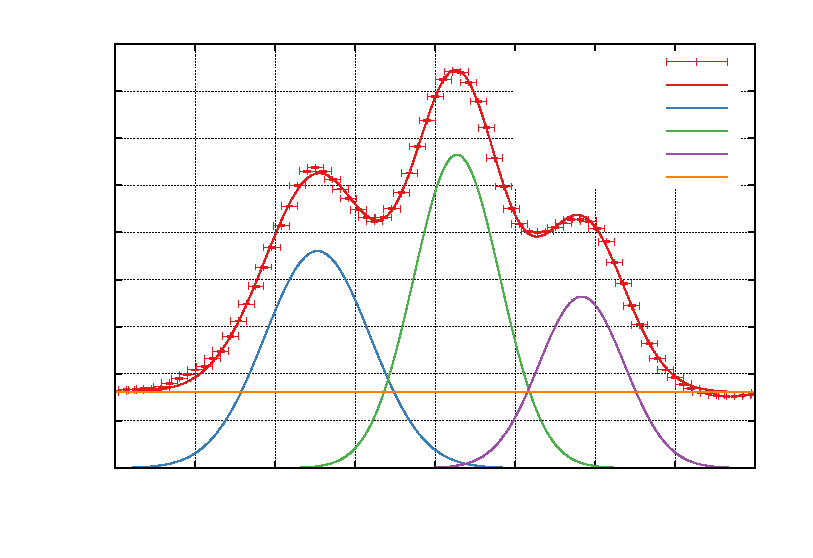
\includegraphics{./plots/zeemann_aufspaltung/b4-5}}%
    \gplfronttext
  \end{picture}%
\endgroup

	}
	\subcaption{}
\end{subfigure}
\\
\begin{subfigure}[c]{0.5\textwidth}
	\scalebox{0.75}{
	% GNUPLOT: LaTeX picture with Postscript
\begingroup
  \makeatletter
  \providecommand\color[2][]{%
    \GenericError{(gnuplot) \space\space\space\@spaces}{%
      Package color not loaded in conjunction with
      terminal option `colourtext'%
    }{See the gnuplot documentation for explanation.%
    }{Either use 'blacktext' in gnuplot or load the package
      color.sty in LaTeX.}%
    \renewcommand\color[2][]{}%
  }%
  \providecommand\includegraphics[2][]{%
    \GenericError{(gnuplot) \space\space\space\@spaces}{%
      Package graphicx or graphics not loaded%
    }{See the gnuplot documentation for explanation.%
    }{The gnuplot epslatex terminal needs graphicx.sty or graphics.sty.}%
    \renewcommand\includegraphics[2][]{}%
  }%
  \providecommand\rotatebox[2]{#2}%
  \@ifundefined{ifGPcolor}{%
    \newif\ifGPcolor
    \GPcolortrue
  }{}%
  \@ifundefined{ifGPblacktext}{%
    \newif\ifGPblacktext
    \GPblacktexttrue
  }{}%
  % define a \g@addto@macro without @ in the name:
  \let\gplgaddtomacro\g@addto@macro
  % define empty templates for all commands taking text:
  \gdef\gplbacktext{}%
  \gdef\gplfronttext{}%
  \makeatother
  \ifGPblacktext
    % no textcolor at all
    \def\colorrgb#1{}%
    \def\colorgray#1{}%
  \else
    % gray or color?
    \ifGPcolor
      \def\colorrgb#1{\color[rgb]{#1}}%
      \def\colorgray#1{\color[gray]{#1}}%
      \expandafter\def\csname LTw\endcsname{\color{white}}%
      \expandafter\def\csname LTb\endcsname{\color{black}}%
      \expandafter\def\csname LTa\endcsname{\color{black}}%
      \expandafter\def\csname LT0\endcsname{\color[rgb]{1,0,0}}%
      \expandafter\def\csname LT1\endcsname{\color[rgb]{0,1,0}}%
      \expandafter\def\csname LT2\endcsname{\color[rgb]{0,0,1}}%
      \expandafter\def\csname LT3\endcsname{\color[rgb]{1,0,1}}%
      \expandafter\def\csname LT4\endcsname{\color[rgb]{0,1,1}}%
      \expandafter\def\csname LT5\endcsname{\color[rgb]{1,1,0}}%
      \expandafter\def\csname LT6\endcsname{\color[rgb]{0,0,0}}%
      \expandafter\def\csname LT7\endcsname{\color[rgb]{1,0.3,0}}%
      \expandafter\def\csname LT8\endcsname{\color[rgb]{0.5,0.5,0.5}}%
    \else
      % gray
      \def\colorrgb#1{\color{black}}%
      \def\colorgray#1{\color[gray]{#1}}%
      \expandafter\def\csname LTw\endcsname{\color{white}}%
      \expandafter\def\csname LTb\endcsname{\color{black}}%
      \expandafter\def\csname LTa\endcsname{\color{black}}%
      \expandafter\def\csname LT0\endcsname{\color{black}}%
      \expandafter\def\csname LT1\endcsname{\color{black}}%
      \expandafter\def\csname LT2\endcsname{\color{black}}%
      \expandafter\def\csname LT3\endcsname{\color{black}}%
      \expandafter\def\csname LT4\endcsname{\color{black}}%
      \expandafter\def\csname LT5\endcsname{\color{black}}%
      \expandafter\def\csname LT6\endcsname{\color{black}}%
      \expandafter\def\csname LT7\endcsname{\color{black}}%
      \expandafter\def\csname LT8\endcsname{\color{black}}%
    \fi
  \fi
  \setlength{\unitlength}{0.0500bp}%
  \begin{picture}(7488.00,5040.00)%
    \gplgaddtomacro\gplbacktext{%
      \csname LTb\endcsname%
      \put(814,704){\makebox(0,0)[r]{\strut{} 0}}%
      \csname LTb\endcsname%
      \put(814,1156){\makebox(0,0)[r]{\strut{} 5}}%
      \csname LTb\endcsname%
      \put(814,1609){\makebox(0,0)[r]{\strut{} 10}}%
      \csname LTb\endcsname%
      \put(814,2061){\makebox(0,0)[r]{\strut{} 15}}%
      \csname LTb\endcsname%
      \put(814,2513){\makebox(0,0)[r]{\strut{} 20}}%
      \csname LTb\endcsname%
      \put(814,2966){\makebox(0,0)[r]{\strut{} 25}}%
      \csname LTb\endcsname%
      \put(814,3418){\makebox(0,0)[r]{\strut{} 30}}%
      \csname LTb\endcsname%
      \put(814,3870){\makebox(0,0)[r]{\strut{} 35}}%
      \csname LTb\endcsname%
      \put(814,4323){\makebox(0,0)[r]{\strut{} 40}}%
      \csname LTb\endcsname%
      \put(814,4775){\makebox(0,0)[r]{\strut{} 45}}%
      \csname LTb\endcsname%
      \put(1655,484){\makebox(0,0){\strut{} 0.9}}%
      \csname LTb\endcsname%
      \put(2837,484){\makebox(0,0){\strut{} 0.95}}%
      \csname LTb\endcsname%
      \put(4019,484){\makebox(0,0){\strut{} 1}}%
      \csname LTb\endcsname%
      \put(5200,484){\makebox(0,0){\strut{} 1.05}}%
      \csname LTb\endcsname%
      \put(6382,484){\makebox(0,0){\strut{} 1.1}}%
      \put(176,2739){\rotatebox{-270}{\makebox(0,0){\strut{}Intensität $I$ / \si{\percent}}}}%
      \put(4018,154){\makebox(0,0){\strut{}Winkel $\alpha$ / \si{\degree}}}%
      \put(4018,4665){\makebox(0,0){\strut{}}}%
    }%
    \gplgaddtomacro\gplfronttext{%
      \csname LTb\endcsname%
      \put(6104,4602){\makebox(0,0)[r]{\strut{}Messwerte}}%
      \csname LTb\endcsname%
      \put(6104,4382){\makebox(0,0)[r]{\strut{}$\Sigma$}}%
      \csname LTb\endcsname%
      \put(6104,4162){\makebox(0,0)[r]{\strut{}$\mathcal{G}_1$}}%
      \csname LTb\endcsname%
      \put(6104,3942){\makebox(0,0)[r]{\strut{}$\mathcal{G}_2$}}%
      \csname LTb\endcsname%
      \put(6104,3722){\makebox(0,0)[r]{\strut{}$\mathcal{G}_3$}}%
      \csname LTb\endcsname%
      \put(6104,3502){\makebox(0,0)[r]{\strut{}Untergrund}}%
    }%
    \gplbacktext
    \put(0,0){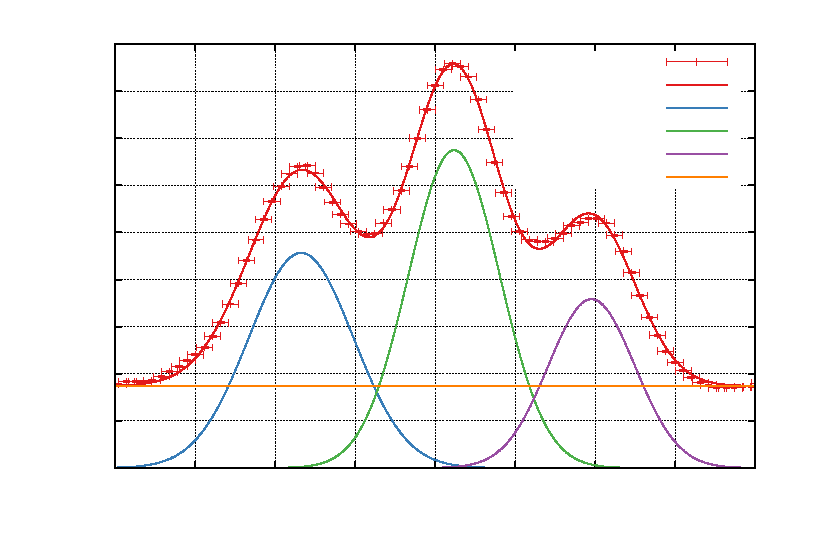
\includegraphics{./plots/zeemann_aufspaltung/b5}}%
    \gplfronttext
  \end{picture}%
\endgroup

	}
	\subcaption{}
\end{subfigure}
\begin{subfigure}[c]{0.5\textwidth}
\scalebox{0.75}{
	% GNUPLOT: LaTeX picture with Postscript
\begingroup
  \makeatletter
  \providecommand\color[2][]{%
    \GenericError{(gnuplot) \space\space\space\@spaces}{%
      Package color not loaded in conjunction with
      terminal option `colourtext'%
    }{See the gnuplot documentation for explanation.%
    }{Either use 'blacktext' in gnuplot or load the package
      color.sty in LaTeX.}%
    \renewcommand\color[2][]{}%
  }%
  \providecommand\includegraphics[2][]{%
    \GenericError{(gnuplot) \space\space\space\@spaces}{%
      Package graphicx or graphics not loaded%
    }{See the gnuplot documentation for explanation.%
    }{The gnuplot epslatex terminal needs graphicx.sty or graphics.sty.}%
    \renewcommand\includegraphics[2][]{}%
  }%
  \providecommand\rotatebox[2]{#2}%
  \@ifundefined{ifGPcolor}{%
    \newif\ifGPcolor
    \GPcolortrue
  }{}%
  \@ifundefined{ifGPblacktext}{%
    \newif\ifGPblacktext
    \GPblacktexttrue
  }{}%
  % define a \g@addto@macro without @ in the name:
  \let\gplgaddtomacro\g@addto@macro
  % define empty templates for all commands taking text:
  \gdef\gplbacktext{}%
  \gdef\gplfronttext{}%
  \makeatother
  \ifGPblacktext
    % no textcolor at all
    \def\colorrgb#1{}%
    \def\colorgray#1{}%
  \else
    % gray or color?
    \ifGPcolor
      \def\colorrgb#1{\color[rgb]{#1}}%
      \def\colorgray#1{\color[gray]{#1}}%
      \expandafter\def\csname LTw\endcsname{\color{white}}%
      \expandafter\def\csname LTb\endcsname{\color{black}}%
      \expandafter\def\csname LTa\endcsname{\color{black}}%
      \expandafter\def\csname LT0\endcsname{\color[rgb]{1,0,0}}%
      \expandafter\def\csname LT1\endcsname{\color[rgb]{0,1,0}}%
      \expandafter\def\csname LT2\endcsname{\color[rgb]{0,0,1}}%
      \expandafter\def\csname LT3\endcsname{\color[rgb]{1,0,1}}%
      \expandafter\def\csname LT4\endcsname{\color[rgb]{0,1,1}}%
      \expandafter\def\csname LT5\endcsname{\color[rgb]{1,1,0}}%
      \expandafter\def\csname LT6\endcsname{\color[rgb]{0,0,0}}%
      \expandafter\def\csname LT7\endcsname{\color[rgb]{1,0.3,0}}%
      \expandafter\def\csname LT8\endcsname{\color[rgb]{0.5,0.5,0.5}}%
    \else
      % gray
      \def\colorrgb#1{\color{black}}%
      \def\colorgray#1{\color[gray]{#1}}%
      \expandafter\def\csname LTw\endcsname{\color{white}}%
      \expandafter\def\csname LTb\endcsname{\color{black}}%
      \expandafter\def\csname LTa\endcsname{\color{black}}%
      \expandafter\def\csname LT0\endcsname{\color{black}}%
      \expandafter\def\csname LT1\endcsname{\color{black}}%
      \expandafter\def\csname LT2\endcsname{\color{black}}%
      \expandafter\def\csname LT3\endcsname{\color{black}}%
      \expandafter\def\csname LT4\endcsname{\color{black}}%
      \expandafter\def\csname LT5\endcsname{\color{black}}%
      \expandafter\def\csname LT6\endcsname{\color{black}}%
      \expandafter\def\csname LT7\endcsname{\color{black}}%
      \expandafter\def\csname LT8\endcsname{\color{black}}%
    \fi
  \fi
  \setlength{\unitlength}{0.0500bp}%
  \begin{picture}(7486.00,5040.00)%
    \gplgaddtomacro\gplbacktext{%
      \csname LTb\endcsname%
      \put(814,704){\makebox(0,0)[r]{\strut{} 0}}%
      \csname LTb\endcsname%
      \put(814,1156){\makebox(0,0)[r]{\strut{} 5}}%
      \csname LTb\endcsname%
      \put(814,1609){\makebox(0,0)[r]{\strut{} 10}}%
      \csname LTb\endcsname%
      \put(814,2061){\makebox(0,0)[r]{\strut{} 15}}%
      \csname LTb\endcsname%
      \put(814,2513){\makebox(0,0)[r]{\strut{} 20}}%
      \csname LTb\endcsname%
      \put(814,2966){\makebox(0,0)[r]{\strut{} 25}}%
      \csname LTb\endcsname%
      \put(814,3418){\makebox(0,0)[r]{\strut{} 30}}%
      \csname LTb\endcsname%
      \put(814,3870){\makebox(0,0)[r]{\strut{} 35}}%
      \csname LTb\endcsname%
      \put(814,4323){\makebox(0,0)[r]{\strut{} 40}}%
      \csname LTb\endcsname%
      \put(814,4775){\makebox(0,0)[r]{\strut{} 45}}%
      \csname LTb\endcsname%
      \put(946,484){\makebox(0,0){\strut{} 0.8}}%
      \csname LTb\endcsname%
      \put(1714,484){\makebox(0,0){\strut{} 0.85}}%
      \csname LTb\endcsname%
      \put(2482,484){\makebox(0,0){\strut{} 0.9}}%
      \csname LTb\endcsname%
      \put(3250,484){\makebox(0,0){\strut{} 0.95}}%
      \csname LTb\endcsname%
      \put(4018,484){\makebox(0,0){\strut{} 1}}%
      \csname LTb\endcsname%
      \put(4785,484){\makebox(0,0){\strut{} 1.05}}%
      \csname LTb\endcsname%
      \put(5553,484){\makebox(0,0){\strut{} 1.1}}%
      \csname LTb\endcsname%
      \put(6321,484){\makebox(0,0){\strut{} 1.15}}%
      \csname LTb\endcsname%
      \put(7089,484){\makebox(0,0){\strut{} 1.2}}%
      \put(176,2739){\rotatebox{-270}{\makebox(0,0){\strut{}Intensität $I$ / \si{\percent}}}}%
      \put(4017,154){\makebox(0,0){\strut{}Winkel $\alpha$ / \si{\degree}}}%
      \put(4017,4665){\makebox(0,0){\strut{}}}%
    }%
    \gplgaddtomacro\gplfronttext{%
      \csname LTb\endcsname%
      \put(6102,4602){\makebox(0,0)[r]{\strut{}Messwerte}}%
      \csname LTb\endcsname%
      \put(6102,4382){\makebox(0,0)[r]{\strut{}$\Sigma$}}%
      \csname LTb\endcsname%
      \put(6102,4162){\makebox(0,0)[r]{\strut{}$\mathcal{G}_1$}}%
      \csname LTb\endcsname%
      \put(6102,3942){\makebox(0,0)[r]{\strut{}$\mathcal{G}_2$}}%
      \csname LTb\endcsname%
      \put(6102,3722){\makebox(0,0)[r]{\strut{}$\mathcal{G}_3$}}%
      \csname LTb\endcsname%
      \put(6102,3502){\makebox(0,0)[r]{\strut{}Untergrund}}%
    }%
    \gplbacktext
    \put(0,0){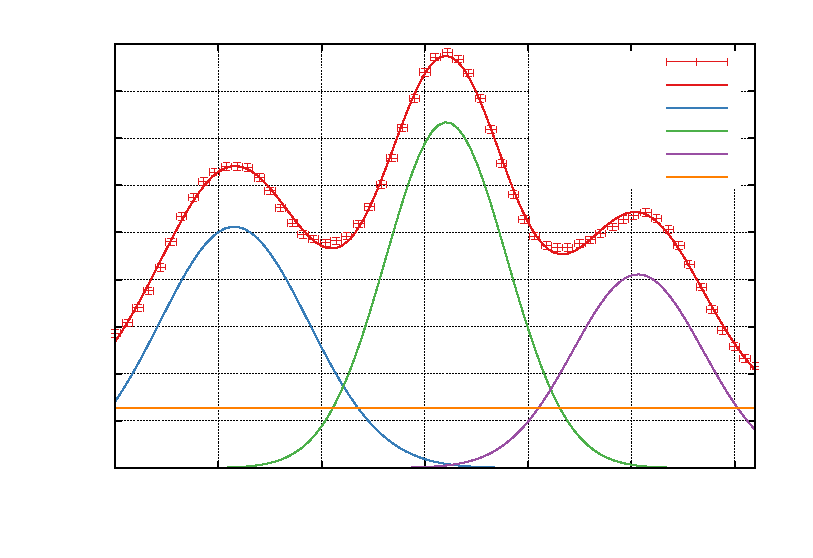
\includegraphics{./plots/zeemann_aufspaltung/b5-5}}%
    \gplfronttext
  \end{picture}%
\endgroup

	}
	\subcaption{}
\end{subfigure}
\caption{Magnetfeldaufspaltung Fits für \textbf{(a)} \SI{4}{\ampere}, \textbf{(b)} \SI{4.5}{\ampere}, \textbf{(c)}) \SI{5}{\ampere}, \textbf{(d)} \SI{5.5}{\ampere}}
\end{sidewaysfigure}

\begin{sidewaysfigure}[!h]
\begin{subfigure}[c]{0.5\textwidth}
\scalebox{0.75}{
	% GNUPLOT: LaTeX picture with Postscript
\begingroup
  \makeatletter
  \providecommand\color[2][]{%
    \GenericError{(gnuplot) \space\space\space\@spaces}{%
      Package color not loaded in conjunction with
      terminal option `colourtext'%
    }{See the gnuplot documentation for explanation.%
    }{Either use 'blacktext' in gnuplot or load the package
      color.sty in LaTeX.}%
    \renewcommand\color[2][]{}%
  }%
  \providecommand\includegraphics[2][]{%
    \GenericError{(gnuplot) \space\space\space\@spaces}{%
      Package graphicx or graphics not loaded%
    }{See the gnuplot documentation for explanation.%
    }{The gnuplot epslatex terminal needs graphicx.sty or graphics.sty.}%
    \renewcommand\includegraphics[2][]{}%
  }%
  \providecommand\rotatebox[2]{#2}%
  \@ifundefined{ifGPcolor}{%
    \newif\ifGPcolor
    \GPcolortrue
  }{}%
  \@ifundefined{ifGPblacktext}{%
    \newif\ifGPblacktext
    \GPblacktexttrue
  }{}%
  % define a \g@addto@macro without @ in the name:
  \let\gplgaddtomacro\g@addto@macro
  % define empty templates for all commands taking text:
  \gdef\gplbacktext{}%
  \gdef\gplfronttext{}%
  \makeatother
  \ifGPblacktext
    % no textcolor at all
    \def\colorrgb#1{}%
    \def\colorgray#1{}%
  \else
    % gray or color?
    \ifGPcolor
      \def\colorrgb#1{\color[rgb]{#1}}%
      \def\colorgray#1{\color[gray]{#1}}%
      \expandafter\def\csname LTw\endcsname{\color{white}}%
      \expandafter\def\csname LTb\endcsname{\color{black}}%
      \expandafter\def\csname LTa\endcsname{\color{black}}%
      \expandafter\def\csname LT0\endcsname{\color[rgb]{1,0,0}}%
      \expandafter\def\csname LT1\endcsname{\color[rgb]{0,1,0}}%
      \expandafter\def\csname LT2\endcsname{\color[rgb]{0,0,1}}%
      \expandafter\def\csname LT3\endcsname{\color[rgb]{1,0,1}}%
      \expandafter\def\csname LT4\endcsname{\color[rgb]{0,1,1}}%
      \expandafter\def\csname LT5\endcsname{\color[rgb]{1,1,0}}%
      \expandafter\def\csname LT6\endcsname{\color[rgb]{0,0,0}}%
      \expandafter\def\csname LT7\endcsname{\color[rgb]{1,0.3,0}}%
      \expandafter\def\csname LT8\endcsname{\color[rgb]{0.5,0.5,0.5}}%
    \else
      % gray
      \def\colorrgb#1{\color{black}}%
      \def\colorgray#1{\color[gray]{#1}}%
      \expandafter\def\csname LTw\endcsname{\color{white}}%
      \expandafter\def\csname LTb\endcsname{\color{black}}%
      \expandafter\def\csname LTa\endcsname{\color{black}}%
      \expandafter\def\csname LT0\endcsname{\color{black}}%
      \expandafter\def\csname LT1\endcsname{\color{black}}%
      \expandafter\def\csname LT2\endcsname{\color{black}}%
      \expandafter\def\csname LT3\endcsname{\color{black}}%
      \expandafter\def\csname LT4\endcsname{\color{black}}%
      \expandafter\def\csname LT5\endcsname{\color{black}}%
      \expandafter\def\csname LT6\endcsname{\color{black}}%
      \expandafter\def\csname LT7\endcsname{\color{black}}%
      \expandafter\def\csname LT8\endcsname{\color{black}}%
    \fi
  \fi
  \setlength{\unitlength}{0.0500bp}%
  \begin{picture}(7486.00,5040.00)%
    \gplgaddtomacro\gplbacktext{%
      \csname LTb\endcsname%
      \put(814,704){\makebox(0,0)[r]{\strut{} 0}}%
      \csname LTb\endcsname%
      \put(814,1111){\makebox(0,0)[r]{\strut{} 5}}%
      \csname LTb\endcsname%
      \put(814,1518){\makebox(0,0)[r]{\strut{} 10}}%
      \csname LTb\endcsname%
      \put(814,1925){\makebox(0,0)[r]{\strut{} 15}}%
      \csname LTb\endcsname%
      \put(814,2332){\makebox(0,0)[r]{\strut{} 20}}%
      \csname LTb\endcsname%
      \put(814,2740){\makebox(0,0)[r]{\strut{} 25}}%
      \csname LTb\endcsname%
      \put(814,3147){\makebox(0,0)[r]{\strut{} 30}}%
      \csname LTb\endcsname%
      \put(814,3554){\makebox(0,0)[r]{\strut{} 35}}%
      \csname LTb\endcsname%
      \put(814,3961){\makebox(0,0)[r]{\strut{} 40}}%
      \csname LTb\endcsname%
      \put(814,4368){\makebox(0,0)[r]{\strut{} 45}}%
      \csname LTb\endcsname%
      \put(814,4775){\makebox(0,0)[r]{\strut{} 50}}%
      \csname LTb\endcsname%
      \put(946,484){\makebox(0,0){\strut{} 0.8}}%
      \csname LTb\endcsname%
      \put(1714,484){\makebox(0,0){\strut{} 0.85}}%
      \csname LTb\endcsname%
      \put(2482,484){\makebox(0,0){\strut{} 0.9}}%
      \csname LTb\endcsname%
      \put(3250,484){\makebox(0,0){\strut{} 0.95}}%
      \csname LTb\endcsname%
      \put(4018,484){\makebox(0,0){\strut{} 1}}%
      \csname LTb\endcsname%
      \put(4785,484){\makebox(0,0){\strut{} 1.05}}%
      \csname LTb\endcsname%
      \put(5553,484){\makebox(0,0){\strut{} 1.1}}%
      \csname LTb\endcsname%
      \put(6321,484){\makebox(0,0){\strut{} 1.15}}%
      \csname LTb\endcsname%
      \put(7089,484){\makebox(0,0){\strut{} 1.2}}%
      \put(176,2739){\rotatebox{-270}{\makebox(0,0){\strut{}Intensität $I$ / \si{\percent}}}}%
      \put(4017,154){\makebox(0,0){\strut{}Winkel $\alpha$ / \si{\degree}}}%
      \put(4017,4665){\makebox(0,0){\strut{}}}%
    }%
    \gplgaddtomacro\gplfronttext{%
      \csname LTb\endcsname%
      \put(6102,4602){\makebox(0,0)[r]{\strut{}Messwerte}}%
      \csname LTb\endcsname%
      \put(6102,4382){\makebox(0,0)[r]{\strut{}$\Sigma$}}%
      \csname LTb\endcsname%
      \put(6102,4162){\makebox(0,0)[r]{\strut{}$\mathcal{G}_1$}}%
      \csname LTb\endcsname%
      \put(6102,3942){\makebox(0,0)[r]{\strut{}$\mathcal{G}_2$}}%
      \csname LTb\endcsname%
      \put(6102,3722){\makebox(0,0)[r]{\strut{}$\mathcal{G}_3$}}%
      \csname LTb\endcsname%
      \put(6102,3502){\makebox(0,0)[r]{\strut{}Untergrund}}%
    }%
    \gplbacktext
    \put(0,0){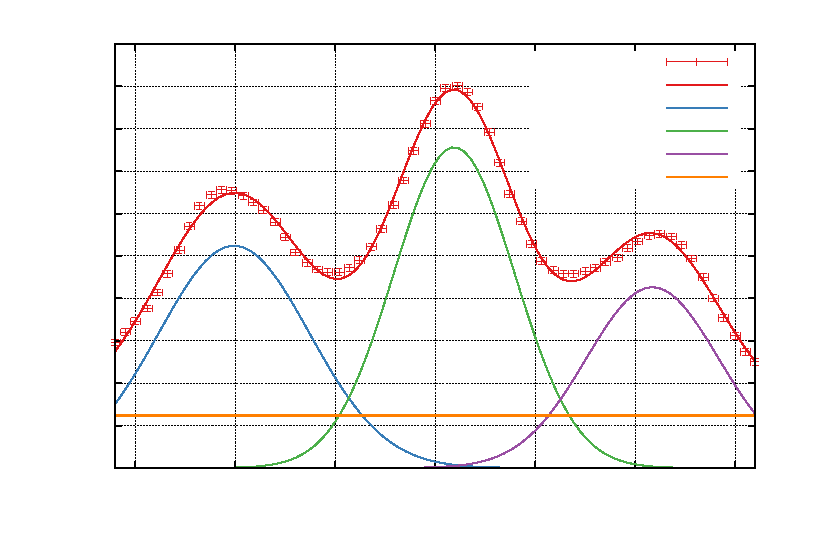
\includegraphics{./plots/zeemann_aufspaltung/b6}}%
    \gplfronttext
  \end{picture}%
\endgroup

	}
	\subcaption{}
\end{subfigure}
\begin{subfigure}[c]{0.5\textwidth}
\scalebox{0.75}{
	% GNUPLOT: LaTeX picture with Postscript
\begingroup
  \makeatletter
  \providecommand\color[2][]{%
    \GenericError{(gnuplot) \space\space\space\@spaces}{%
      Package color not loaded in conjunction with
      terminal option `colourtext'%
    }{See the gnuplot documentation for explanation.%
    }{Either use 'blacktext' in gnuplot or load the package
      color.sty in LaTeX.}%
    \renewcommand\color[2][]{}%
  }%
  \providecommand\includegraphics[2][]{%
    \GenericError{(gnuplot) \space\space\space\@spaces}{%
      Package graphicx or graphics not loaded%
    }{See the gnuplot documentation for explanation.%
    }{The gnuplot epslatex terminal needs graphicx.sty or graphics.sty.}%
    \renewcommand\includegraphics[2][]{}%
  }%
  \providecommand\rotatebox[2]{#2}%
  \@ifundefined{ifGPcolor}{%
    \newif\ifGPcolor
    \GPcolortrue
  }{}%
  \@ifundefined{ifGPblacktext}{%
    \newif\ifGPblacktext
    \GPblacktexttrue
  }{}%
  % define a \g@addto@macro without @ in the name:
  \let\gplgaddtomacro\g@addto@macro
  % define empty templates for all commands taking text:
  \gdef\gplbacktext{}%
  \gdef\gplfronttext{}%
  \makeatother
  \ifGPblacktext
    % no textcolor at all
    \def\colorrgb#1{}%
    \def\colorgray#1{}%
  \else
    % gray or color?
    \ifGPcolor
      \def\colorrgb#1{\color[rgb]{#1}}%
      \def\colorgray#1{\color[gray]{#1}}%
      \expandafter\def\csname LTw\endcsname{\color{white}}%
      \expandafter\def\csname LTb\endcsname{\color{black}}%
      \expandafter\def\csname LTa\endcsname{\color{black}}%
      \expandafter\def\csname LT0\endcsname{\color[rgb]{1,0,0}}%
      \expandafter\def\csname LT1\endcsname{\color[rgb]{0,1,0}}%
      \expandafter\def\csname LT2\endcsname{\color[rgb]{0,0,1}}%
      \expandafter\def\csname LT3\endcsname{\color[rgb]{1,0,1}}%
      \expandafter\def\csname LT4\endcsname{\color[rgb]{0,1,1}}%
      \expandafter\def\csname LT5\endcsname{\color[rgb]{1,1,0}}%
      \expandafter\def\csname LT6\endcsname{\color[rgb]{0,0,0}}%
      \expandafter\def\csname LT7\endcsname{\color[rgb]{1,0.3,0}}%
      \expandafter\def\csname LT8\endcsname{\color[rgb]{0.5,0.5,0.5}}%
    \else
      % gray
      \def\colorrgb#1{\color{black}}%
      \def\colorgray#1{\color[gray]{#1}}%
      \expandafter\def\csname LTw\endcsname{\color{white}}%
      \expandafter\def\csname LTb\endcsname{\color{black}}%
      \expandafter\def\csname LTa\endcsname{\color{black}}%
      \expandafter\def\csname LT0\endcsname{\color{black}}%
      \expandafter\def\csname LT1\endcsname{\color{black}}%
      \expandafter\def\csname LT2\endcsname{\color{black}}%
      \expandafter\def\csname LT3\endcsname{\color{black}}%
      \expandafter\def\csname LT4\endcsname{\color{black}}%
      \expandafter\def\csname LT5\endcsname{\color{black}}%
      \expandafter\def\csname LT6\endcsname{\color{black}}%
      \expandafter\def\csname LT7\endcsname{\color{black}}%
      \expandafter\def\csname LT8\endcsname{\color{black}}%
    \fi
  \fi
  \setlength{\unitlength}{0.0500bp}%
  \begin{picture}(7488.00,5040.00)%
    \gplgaddtomacro\gplbacktext{%
      \csname LTb\endcsname%
      \put(814,704){\makebox(0,0)[r]{\strut{} 0}}%
      \csname LTb\endcsname%
      \put(814,1111){\makebox(0,0)[r]{\strut{} 5}}%
      \csname LTb\endcsname%
      \put(814,1518){\makebox(0,0)[r]{\strut{} 10}}%
      \csname LTb\endcsname%
      \put(814,1925){\makebox(0,0)[r]{\strut{} 15}}%
      \csname LTb\endcsname%
      \put(814,2332){\makebox(0,0)[r]{\strut{} 20}}%
      \csname LTb\endcsname%
      \put(814,2740){\makebox(0,0)[r]{\strut{} 25}}%
      \csname LTb\endcsname%
      \put(814,3147){\makebox(0,0)[r]{\strut{} 30}}%
      \csname LTb\endcsname%
      \put(814,3554){\makebox(0,0)[r]{\strut{} 35}}%
      \csname LTb\endcsname%
      \put(814,3961){\makebox(0,0)[r]{\strut{} 40}}%
      \csname LTb\endcsname%
      \put(814,4368){\makebox(0,0)[r]{\strut{} 45}}%
      \csname LTb\endcsname%
      \put(814,4775){\makebox(0,0)[r]{\strut{} 50}}%
      \csname LTb\endcsname%
      \put(1307,484){\makebox(0,0){\strut{} 0.85}}%
      \csname LTb\endcsname%
      \put(2211,484){\makebox(0,0){\strut{} 0.9}}%
      \csname LTb\endcsname%
      \put(3115,484){\makebox(0,0){\strut{} 0.95}}%
      \csname LTb\endcsname%
      \put(4019,484){\makebox(0,0){\strut{} 1}}%
      \csname LTb\endcsname%
      \put(4922,484){\makebox(0,0){\strut{} 1.05}}%
      \csname LTb\endcsname%
      \put(5826,484){\makebox(0,0){\strut{} 1.1}}%
      \csname LTb\endcsname%
      \put(6730,484){\makebox(0,0){\strut{} 1.15}}%
      \put(176,2739){\rotatebox{-270}{\makebox(0,0){\strut{}Intensität $I$ / \si{\percent}}}}%
      \put(4018,154){\makebox(0,0){\strut{}Winkel $\alpha$ / \si{\degree}}}%
      \put(4018,4665){\makebox(0,0){\strut{}}}%
    }%
    \gplgaddtomacro\gplfronttext{%
      \csname LTb\endcsname%
      \put(6104,4602){\makebox(0,0)[r]{\strut{}Messwerte}}%
      \csname LTb\endcsname%
      \put(6104,4382){\makebox(0,0)[r]{\strut{}$\Sigma$}}%
      \csname LTb\endcsname%
      \put(6104,4162){\makebox(0,0)[r]{\strut{}$\mathcal{G}_1$}}%
      \csname LTb\endcsname%
      \put(6104,3942){\makebox(0,0)[r]{\strut{}$\mathcal{G}_2$}}%
      \csname LTb\endcsname%
      \put(6104,3722){\makebox(0,0)[r]{\strut{}$\mathcal{G}_3$}}%
      \csname LTb\endcsname%
      \put(6104,3502){\makebox(0,0)[r]{\strut{}$d$}}%
    }%
    \gplbacktext
    \put(0,0){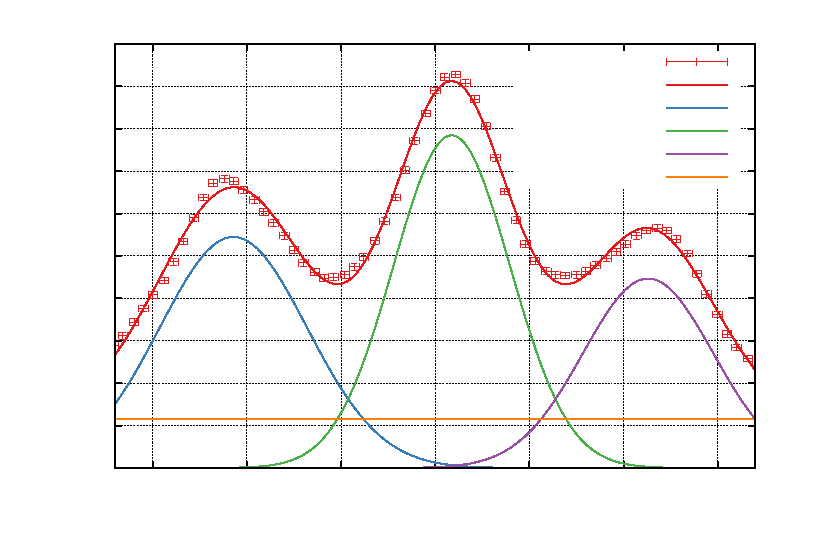
\includegraphics{./plots/zeemann_aufspaltung/b6-5}}%
    \gplfronttext
  \end{picture}%
\endgroup

	}
	\subcaption{}
\end{subfigure}
\\
\begin{subfigure}[c]{0.5\textwidth}
	\scalebox{0.75}{
	% GNUPLOT: LaTeX picture with Postscript
\begingroup
  \makeatletter
  \providecommand\color[2][]{%
    \GenericError{(gnuplot) \space\space\space\@spaces}{%
      Package color not loaded in conjunction with
      terminal option `colourtext'%
    }{See the gnuplot documentation for explanation.%
    }{Either use 'blacktext' in gnuplot or load the package
      color.sty in LaTeX.}%
    \renewcommand\color[2][]{}%
  }%
  \providecommand\includegraphics[2][]{%
    \GenericError{(gnuplot) \space\space\space\@spaces}{%
      Package graphicx or graphics not loaded%
    }{See the gnuplot documentation for explanation.%
    }{The gnuplot epslatex terminal needs graphicx.sty or graphics.sty.}%
    \renewcommand\includegraphics[2][]{}%
  }%
  \providecommand\rotatebox[2]{#2}%
  \@ifundefined{ifGPcolor}{%
    \newif\ifGPcolor
    \GPcolortrue
  }{}%
  \@ifundefined{ifGPblacktext}{%
    \newif\ifGPblacktext
    \GPblacktexttrue
  }{}%
  % define a \g@addto@macro without @ in the name:
  \let\gplgaddtomacro\g@addto@macro
  % define empty templates for all commands taking text:
  \gdef\gplbacktext{}%
  \gdef\gplfronttext{}%
  \makeatother
  \ifGPblacktext
    % no textcolor at all
    \def\colorrgb#1{}%
    \def\colorgray#1{}%
  \else
    % gray or color?
    \ifGPcolor
      \def\colorrgb#1{\color[rgb]{#1}}%
      \def\colorgray#1{\color[gray]{#1}}%
      \expandafter\def\csname LTw\endcsname{\color{white}}%
      \expandafter\def\csname LTb\endcsname{\color{black}}%
      \expandafter\def\csname LTa\endcsname{\color{black}}%
      \expandafter\def\csname LT0\endcsname{\color[rgb]{1,0,0}}%
      \expandafter\def\csname LT1\endcsname{\color[rgb]{0,1,0}}%
      \expandafter\def\csname LT2\endcsname{\color[rgb]{0,0,1}}%
      \expandafter\def\csname LT3\endcsname{\color[rgb]{1,0,1}}%
      \expandafter\def\csname LT4\endcsname{\color[rgb]{0,1,1}}%
      \expandafter\def\csname LT5\endcsname{\color[rgb]{1,1,0}}%
      \expandafter\def\csname LT6\endcsname{\color[rgb]{0,0,0}}%
      \expandafter\def\csname LT7\endcsname{\color[rgb]{1,0.3,0}}%
      \expandafter\def\csname LT8\endcsname{\color[rgb]{0.5,0.5,0.5}}%
    \else
      % gray
      \def\colorrgb#1{\color{black}}%
      \def\colorgray#1{\color[gray]{#1}}%
      \expandafter\def\csname LTw\endcsname{\color{white}}%
      \expandafter\def\csname LTb\endcsname{\color{black}}%
      \expandafter\def\csname LTa\endcsname{\color{black}}%
      \expandafter\def\csname LT0\endcsname{\color{black}}%
      \expandafter\def\csname LT1\endcsname{\color{black}}%
      \expandafter\def\csname LT2\endcsname{\color{black}}%
      \expandafter\def\csname LT3\endcsname{\color{black}}%
      \expandafter\def\csname LT4\endcsname{\color{black}}%
      \expandafter\def\csname LT5\endcsname{\color{black}}%
      \expandafter\def\csname LT6\endcsname{\color{black}}%
      \expandafter\def\csname LT7\endcsname{\color{black}}%
      \expandafter\def\csname LT8\endcsname{\color{black}}%
    \fi
  \fi
  \setlength{\unitlength}{0.0500bp}%
  \begin{picture}(7486.00,5040.00)%
    \gplgaddtomacro\gplbacktext{%
      \csname LTb\endcsname%
      \put(814,704){\makebox(0,0)[r]{\strut{} 0}}%
      \csname LTb\endcsname%
      \put(814,1111){\makebox(0,0)[r]{\strut{} 5}}%
      \csname LTb\endcsname%
      \put(814,1518){\makebox(0,0)[r]{\strut{} 10}}%
      \csname LTb\endcsname%
      \put(814,1925){\makebox(0,0)[r]{\strut{} 15}}%
      \csname LTb\endcsname%
      \put(814,2332){\makebox(0,0)[r]{\strut{} 20}}%
      \csname LTb\endcsname%
      \put(814,2740){\makebox(0,0)[r]{\strut{} 25}}%
      \csname LTb\endcsname%
      \put(814,3147){\makebox(0,0)[r]{\strut{} 30}}%
      \csname LTb\endcsname%
      \put(814,3554){\makebox(0,0)[r]{\strut{} 35}}%
      \csname LTb\endcsname%
      \put(814,3961){\makebox(0,0)[r]{\strut{} 40}}%
      \csname LTb\endcsname%
      \put(814,4368){\makebox(0,0)[r]{\strut{} 45}}%
      \csname LTb\endcsname%
      \put(814,4775){\makebox(0,0)[r]{\strut{} 50}}%
      \csname LTb\endcsname%
      \put(946,484){\makebox(0,0){\strut{} 0.8}}%
      \csname LTb\endcsname%
      \put(1714,484){\makebox(0,0){\strut{} 0.85}}%
      \csname LTb\endcsname%
      \put(2482,484){\makebox(0,0){\strut{} 0.9}}%
      \csname LTb\endcsname%
      \put(3250,484){\makebox(0,0){\strut{} 0.95}}%
      \csname LTb\endcsname%
      \put(4018,484){\makebox(0,0){\strut{} 1}}%
      \csname LTb\endcsname%
      \put(4785,484){\makebox(0,0){\strut{} 1.05}}%
      \csname LTb\endcsname%
      \put(5553,484){\makebox(0,0){\strut{} 1.1}}%
      \csname LTb\endcsname%
      \put(6321,484){\makebox(0,0){\strut{} 1.15}}%
      \csname LTb\endcsname%
      \put(7089,484){\makebox(0,0){\strut{} 1.2}}%
      \put(176,2739){\rotatebox{-270}{\makebox(0,0){\strut{}Intensität $I$ / \si{\percent}}}}%
      \put(4017,154){\makebox(0,0){\strut{}Winkel $\alpha$ / \si{\degree}}}%
      \put(4017,4665){\makebox(0,0){\strut{}}}%
    }%
    \gplgaddtomacro\gplfronttext{%
      \csname LTb\endcsname%
      \put(6102,4602){\makebox(0,0)[r]{\strut{}Messwerte}}%
      \csname LTb\endcsname%
      \put(6102,4382){\makebox(0,0)[r]{\strut{}$\Sigma$}}%
      \csname LTb\endcsname%
      \put(6102,4162){\makebox(0,0)[r]{\strut{}$\mathcal{G}_1$}}%
      \csname LTb\endcsname%
      \put(6102,3942){\makebox(0,0)[r]{\strut{}$\mathcal{G}_2$}}%
      \csname LTb\endcsname%
      \put(6102,3722){\makebox(0,0)[r]{\strut{}$\mathcal{G}_3$}}%
      \csname LTb\endcsname%
      \put(6102,3502){\makebox(0,0)[r]{\strut{}Untergrund}}%
    }%
    \gplbacktext
    \put(0,0){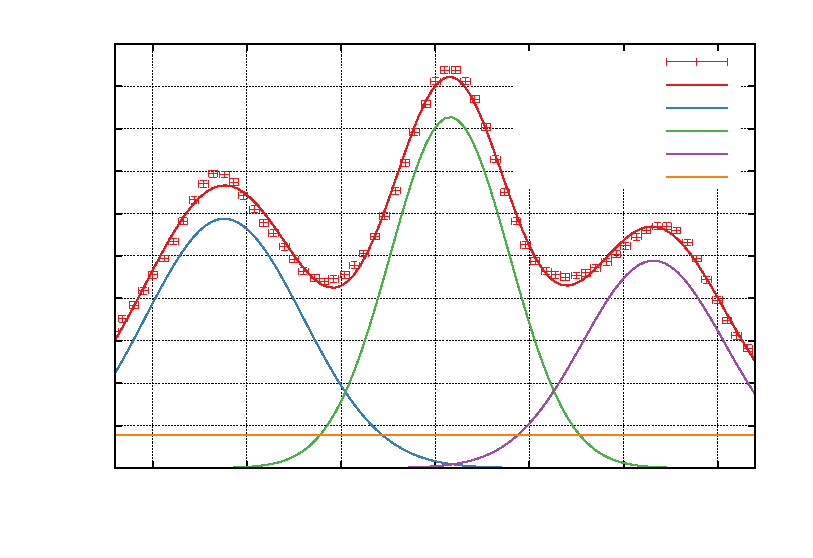
\includegraphics{./plots/zeemann_aufspaltung/b7}}%
    \gplfronttext
  \end{picture}%
\endgroup

	}
	\subcaption{}
\end{subfigure}
\begin{subfigure}[c]{0.5\textwidth}
\scalebox{0.75}{
	% GNUPLOT: LaTeX picture with Postscript
\begingroup
  \makeatletter
  \providecommand\color[2][]{%
    \GenericError{(gnuplot) \space\space\space\@spaces}{%
      Package color not loaded in conjunction with
      terminal option `colourtext'%
    }{See the gnuplot documentation for explanation.%
    }{Either use 'blacktext' in gnuplot or load the package
      color.sty in LaTeX.}%
    \renewcommand\color[2][]{}%
  }%
  \providecommand\includegraphics[2][]{%
    \GenericError{(gnuplot) \space\space\space\@spaces}{%
      Package graphicx or graphics not loaded%
    }{See the gnuplot documentation for explanation.%
    }{The gnuplot epslatex terminal needs graphicx.sty or graphics.sty.}%
    \renewcommand\includegraphics[2][]{}%
  }%
  \providecommand\rotatebox[2]{#2}%
  \@ifundefined{ifGPcolor}{%
    \newif\ifGPcolor
    \GPcolortrue
  }{}%
  \@ifundefined{ifGPblacktext}{%
    \newif\ifGPblacktext
    \GPblacktexttrue
  }{}%
  % define a \g@addto@macro without @ in the name:
  \let\gplgaddtomacro\g@addto@macro
  % define empty templates for all commands taking text:
  \gdef\gplbacktext{}%
  \gdef\gplfronttext{}%
  \makeatother
  \ifGPblacktext
    % no textcolor at all
    \def\colorrgb#1{}%
    \def\colorgray#1{}%
  \else
    % gray or color?
    \ifGPcolor
      \def\colorrgb#1{\color[rgb]{#1}}%
      \def\colorgray#1{\color[gray]{#1}}%
      \expandafter\def\csname LTw\endcsname{\color{white}}%
      \expandafter\def\csname LTb\endcsname{\color{black}}%
      \expandafter\def\csname LTa\endcsname{\color{black}}%
      \expandafter\def\csname LT0\endcsname{\color[rgb]{1,0,0}}%
      \expandafter\def\csname LT1\endcsname{\color[rgb]{0,1,0}}%
      \expandafter\def\csname LT2\endcsname{\color[rgb]{0,0,1}}%
      \expandafter\def\csname LT3\endcsname{\color[rgb]{1,0,1}}%
      \expandafter\def\csname LT4\endcsname{\color[rgb]{0,1,1}}%
      \expandafter\def\csname LT5\endcsname{\color[rgb]{1,1,0}}%
      \expandafter\def\csname LT6\endcsname{\color[rgb]{0,0,0}}%
      \expandafter\def\csname LT7\endcsname{\color[rgb]{1,0.3,0}}%
      \expandafter\def\csname LT8\endcsname{\color[rgb]{0.5,0.5,0.5}}%
    \else
      % gray
      \def\colorrgb#1{\color{black}}%
      \def\colorgray#1{\color[gray]{#1}}%
      \expandafter\def\csname LTw\endcsname{\color{white}}%
      \expandafter\def\csname LTb\endcsname{\color{black}}%
      \expandafter\def\csname LTa\endcsname{\color{black}}%
      \expandafter\def\csname LT0\endcsname{\color{black}}%
      \expandafter\def\csname LT1\endcsname{\color{black}}%
      \expandafter\def\csname LT2\endcsname{\color{black}}%
      \expandafter\def\csname LT3\endcsname{\color{black}}%
      \expandafter\def\csname LT4\endcsname{\color{black}}%
      \expandafter\def\csname LT5\endcsname{\color{black}}%
      \expandafter\def\csname LT6\endcsname{\color{black}}%
      \expandafter\def\csname LT7\endcsname{\color{black}}%
      \expandafter\def\csname LT8\endcsname{\color{black}}%
    \fi
  \fi
  \setlength{\unitlength}{0.0500bp}%
  \begin{picture}(7488.00,5040.00)%
    \gplgaddtomacro\gplbacktext{%
      \csname LTb\endcsname%
      \put(814,704){\makebox(0,0)[r]{\strut{} 0}}%
      \csname LTb\endcsname%
      \put(814,1111){\makebox(0,0)[r]{\strut{} 5}}%
      \csname LTb\endcsname%
      \put(814,1518){\makebox(0,0)[r]{\strut{} 10}}%
      \csname LTb\endcsname%
      \put(814,1925){\makebox(0,0)[r]{\strut{} 15}}%
      \csname LTb\endcsname%
      \put(814,2332){\makebox(0,0)[r]{\strut{} 20}}%
      \csname LTb\endcsname%
      \put(814,2740){\makebox(0,0)[r]{\strut{} 25}}%
      \csname LTb\endcsname%
      \put(814,3147){\makebox(0,0)[r]{\strut{} 30}}%
      \csname LTb\endcsname%
      \put(814,3554){\makebox(0,0)[r]{\strut{} 35}}%
      \csname LTb\endcsname%
      \put(814,3961){\makebox(0,0)[r]{\strut{} 40}}%
      \csname LTb\endcsname%
      \put(814,4368){\makebox(0,0)[r]{\strut{} 45}}%
      \csname LTb\endcsname%
      \put(814,4775){\makebox(0,0)[r]{\strut{} 50}}%
      \csname LTb\endcsname%
      \put(1307,484){\makebox(0,0){\strut{} 0.85}}%
      \csname LTb\endcsname%
      \put(2211,484){\makebox(0,0){\strut{} 0.9}}%
      \csname LTb\endcsname%
      \put(3115,484){\makebox(0,0){\strut{} 0.95}}%
      \csname LTb\endcsname%
      \put(4019,484){\makebox(0,0){\strut{} 1}}%
      \csname LTb\endcsname%
      \put(4922,484){\makebox(0,0){\strut{} 1.05}}%
      \csname LTb\endcsname%
      \put(5826,484){\makebox(0,0){\strut{} 1.1}}%
      \csname LTb\endcsname%
      \put(6730,484){\makebox(0,0){\strut{} 1.15}}%
      \put(176,2739){\rotatebox{-270}{\makebox(0,0){\strut{}Intensität $I$ / \si{\percent}}}}%
      \put(4018,154){\makebox(0,0){\strut{}Winkel $\alpha$ / \si{\degree}}}%
      \put(4018,4665){\makebox(0,0){\strut{}}}%
    }%
    \gplgaddtomacro\gplfronttext{%
      \csname LTb\endcsname%
      \put(6104,4602){\makebox(0,0)[r]{\strut{}Messwerte}}%
      \csname LTb\endcsname%
      \put(6104,4382){\makebox(0,0)[r]{\strut{}$\Sigma$}}%
      \csname LTb\endcsname%
      \put(6104,4162){\makebox(0,0)[r]{\strut{}$\mathcal{G}_1$}}%
      \csname LTb\endcsname%
      \put(6104,3942){\makebox(0,0)[r]{\strut{}$\mathcal{G}_2$}}%
      \csname LTb\endcsname%
      \put(6104,3722){\makebox(0,0)[r]{\strut{}$\mathcal{G}_3$}}%
      \csname LTb\endcsname%
      \put(6104,3502){\makebox(0,0)[r]{\strut{}$d$}}%
    }%
    \gplbacktext
    \put(0,0){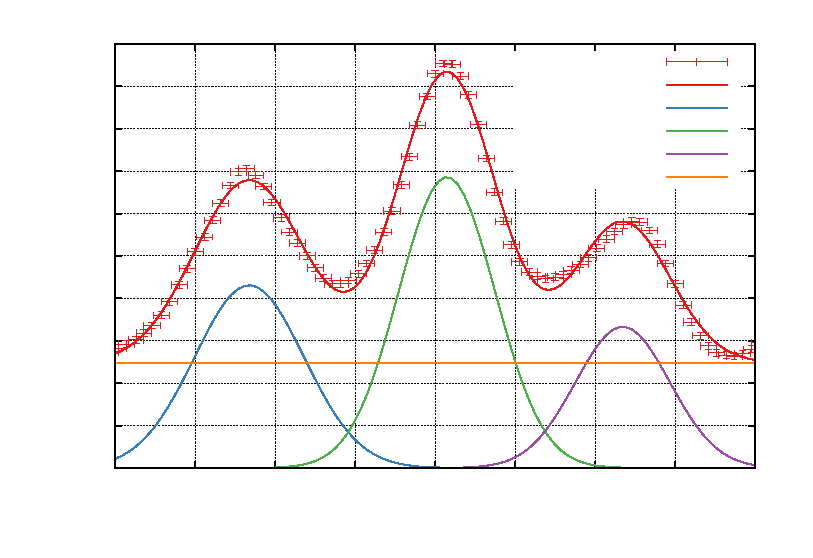
\includegraphics{./plots/zeemann_aufspaltung/b7-5}}%
    \gplfronttext
  \end{picture}%
\endgroup

	}
	\subcaption{}
\end{subfigure}
\caption{Magnetfeldaufspaltung Fits für \textbf{(a)} \SI{6}{\ampere}, \textbf{(b)} \SI{6.5}{\ampere}, \textbf{(c)}) \SI{7}{\ampere}, \textbf{(d)} \SI{7.5}{\ampere}}
\end{sidewaysfigure}

\begin{sidewaysfigure}[!h]
\begin{subfigure}[c]{0.5\textwidth}
\scalebox{0.75}{
	% GNUPLOT: LaTeX picture with Postscript
\begingroup
  \makeatletter
  \providecommand\color[2][]{%
    \GenericError{(gnuplot) \space\space\space\@spaces}{%
      Package color not loaded in conjunction with
      terminal option `colourtext'%
    }{See the gnuplot documentation for explanation.%
    }{Either use 'blacktext' in gnuplot or load the package
      color.sty in LaTeX.}%
    \renewcommand\color[2][]{}%
  }%
  \providecommand\includegraphics[2][]{%
    \GenericError{(gnuplot) \space\space\space\@spaces}{%
      Package graphicx or graphics not loaded%
    }{See the gnuplot documentation for explanation.%
    }{The gnuplot epslatex terminal needs graphicx.sty or graphics.sty.}%
    \renewcommand\includegraphics[2][]{}%
  }%
  \providecommand\rotatebox[2]{#2}%
  \@ifundefined{ifGPcolor}{%
    \newif\ifGPcolor
    \GPcolortrue
  }{}%
  \@ifundefined{ifGPblacktext}{%
    \newif\ifGPblacktext
    \GPblacktexttrue
  }{}%
  % define a \g@addto@macro without @ in the name:
  \let\gplgaddtomacro\g@addto@macro
  % define empty templates for all commands taking text:
  \gdef\gplbacktext{}%
  \gdef\gplfronttext{}%
  \makeatother
  \ifGPblacktext
    % no textcolor at all
    \def\colorrgb#1{}%
    \def\colorgray#1{}%
  \else
    % gray or color?
    \ifGPcolor
      \def\colorrgb#1{\color[rgb]{#1}}%
      \def\colorgray#1{\color[gray]{#1}}%
      \expandafter\def\csname LTw\endcsname{\color{white}}%
      \expandafter\def\csname LTb\endcsname{\color{black}}%
      \expandafter\def\csname LTa\endcsname{\color{black}}%
      \expandafter\def\csname LT0\endcsname{\color[rgb]{1,0,0}}%
      \expandafter\def\csname LT1\endcsname{\color[rgb]{0,1,0}}%
      \expandafter\def\csname LT2\endcsname{\color[rgb]{0,0,1}}%
      \expandafter\def\csname LT3\endcsname{\color[rgb]{1,0,1}}%
      \expandafter\def\csname LT4\endcsname{\color[rgb]{0,1,1}}%
      \expandafter\def\csname LT5\endcsname{\color[rgb]{1,1,0}}%
      \expandafter\def\csname LT6\endcsname{\color[rgb]{0,0,0}}%
      \expandafter\def\csname LT7\endcsname{\color[rgb]{1,0.3,0}}%
      \expandafter\def\csname LT8\endcsname{\color[rgb]{0.5,0.5,0.5}}%
    \else
      % gray
      \def\colorrgb#1{\color{black}}%
      \def\colorgray#1{\color[gray]{#1}}%
      \expandafter\def\csname LTw\endcsname{\color{white}}%
      \expandafter\def\csname LTb\endcsname{\color{black}}%
      \expandafter\def\csname LTa\endcsname{\color{black}}%
      \expandafter\def\csname LT0\endcsname{\color{black}}%
      \expandafter\def\csname LT1\endcsname{\color{black}}%
      \expandafter\def\csname LT2\endcsname{\color{black}}%
      \expandafter\def\csname LT3\endcsname{\color{black}}%
      \expandafter\def\csname LT4\endcsname{\color{black}}%
      \expandafter\def\csname LT5\endcsname{\color{black}}%
      \expandafter\def\csname LT6\endcsname{\color{black}}%
      \expandafter\def\csname LT7\endcsname{\color{black}}%
      \expandafter\def\csname LT8\endcsname{\color{black}}%
    \fi
  \fi
  \setlength{\unitlength}{0.0500bp}%
  \begin{picture}(7486.00,5040.00)%
    \gplgaddtomacro\gplbacktext{%
      \csname LTb\endcsname%
      \put(814,704){\makebox(0,0)[r]{\strut{} 0}}%
      \csname LTb\endcsname%
      \put(814,1111){\makebox(0,0)[r]{\strut{} 5}}%
      \csname LTb\endcsname%
      \put(814,1518){\makebox(0,0)[r]{\strut{} 10}}%
      \csname LTb\endcsname%
      \put(814,1925){\makebox(0,0)[r]{\strut{} 15}}%
      \csname LTb\endcsname%
      \put(814,2332){\makebox(0,0)[r]{\strut{} 20}}%
      \csname LTb\endcsname%
      \put(814,2740){\makebox(0,0)[r]{\strut{} 25}}%
      \csname LTb\endcsname%
      \put(814,3147){\makebox(0,0)[r]{\strut{} 30}}%
      \csname LTb\endcsname%
      \put(814,3554){\makebox(0,0)[r]{\strut{} 35}}%
      \csname LTb\endcsname%
      \put(814,3961){\makebox(0,0)[r]{\strut{} 40}}%
      \csname LTb\endcsname%
      \put(814,4368){\makebox(0,0)[r]{\strut{} 45}}%
      \csname LTb\endcsname%
      \put(814,4775){\makebox(0,0)[r]{\strut{} 50}}%
      \csname LTb\endcsname%
      \put(946,484){\makebox(0,0){\strut{} 0.8}}%
      \csname LTb\endcsname%
      \put(1714,484){\makebox(0,0){\strut{} 0.85}}%
      \csname LTb\endcsname%
      \put(2482,484){\makebox(0,0){\strut{} 0.9}}%
      \csname LTb\endcsname%
      \put(3250,484){\makebox(0,0){\strut{} 0.95}}%
      \csname LTb\endcsname%
      \put(4018,484){\makebox(0,0){\strut{} 1}}%
      \csname LTb\endcsname%
      \put(4785,484){\makebox(0,0){\strut{} 1.05}}%
      \csname LTb\endcsname%
      \put(5553,484){\makebox(0,0){\strut{} 1.1}}%
      \csname LTb\endcsname%
      \put(6321,484){\makebox(0,0){\strut{} 1.15}}%
      \csname LTb\endcsname%
      \put(7089,484){\makebox(0,0){\strut{} 1.2}}%
      \put(176,2739){\rotatebox{-270}{\makebox(0,0){\strut{}Intensität $I$ / \si{\percent}}}}%
      \put(4017,154){\makebox(0,0){\strut{}Winkel $\alpha$ / \si{\degree}}}%
      \put(4017,4665){\makebox(0,0){\strut{}}}%
    }%
    \gplgaddtomacro\gplfronttext{%
      \csname LTb\endcsname%
      \put(6102,4602){\makebox(0,0)[r]{\strut{}Messwerte}}%
      \csname LTb\endcsname%
      \put(6102,4382){\makebox(0,0)[r]{\strut{}$\Sigma$}}%
      \csname LTb\endcsname%
      \put(6102,4162){\makebox(0,0)[r]{\strut{}$\mathcal{G}_1$}}%
      \csname LTb\endcsname%
      \put(6102,3942){\makebox(0,0)[r]{\strut{}$\mathcal{G}_2$}}%
      \csname LTb\endcsname%
      \put(6102,3722){\makebox(0,0)[r]{\strut{}$\mathcal{G}_3$}}%
      \csname LTb\endcsname%
      \put(6102,3502){\makebox(0,0)[r]{\strut{}Untergrund}}%
    }%
    \gplbacktext
    \put(0,0){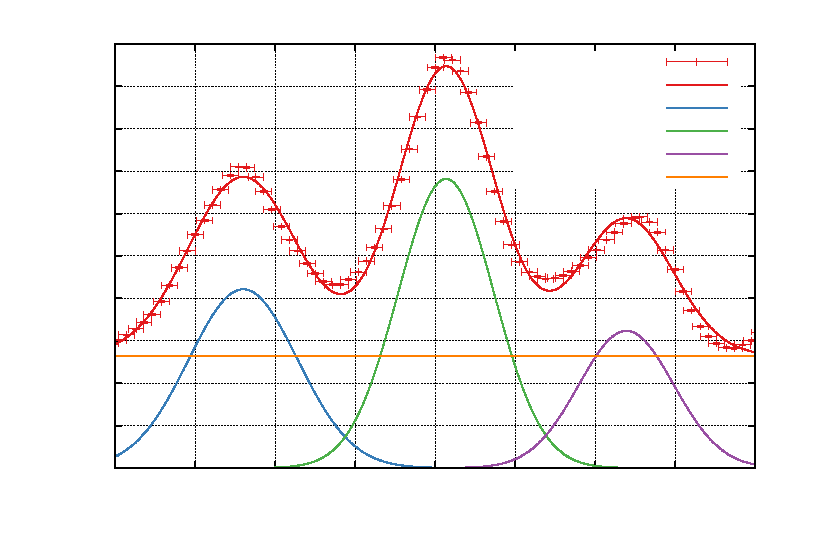
\includegraphics{./plots/zeemann_aufspaltung/b8}}%
    \gplfronttext
  \end{picture}%
\endgroup

	}
	\subcaption{}
\end{subfigure}
\begin{subfigure}[c]{0.5\textwidth}
\scalebox{0.75}{
	% GNUPLOT: LaTeX picture with Postscript
\begingroup
  \makeatletter
  \providecommand\color[2][]{%
    \GenericError{(gnuplot) \space\space\space\@spaces}{%
      Package color not loaded in conjunction with
      terminal option `colourtext'%
    }{See the gnuplot documentation for explanation.%
    }{Either use 'blacktext' in gnuplot or load the package
      color.sty in LaTeX.}%
    \renewcommand\color[2][]{}%
  }%
  \providecommand\includegraphics[2][]{%
    \GenericError{(gnuplot) \space\space\space\@spaces}{%
      Package graphicx or graphics not loaded%
    }{See the gnuplot documentation for explanation.%
    }{The gnuplot epslatex terminal needs graphicx.sty or graphics.sty.}%
    \renewcommand\includegraphics[2][]{}%
  }%
  \providecommand\rotatebox[2]{#2}%
  \@ifundefined{ifGPcolor}{%
    \newif\ifGPcolor
    \GPcolortrue
  }{}%
  \@ifundefined{ifGPblacktext}{%
    \newif\ifGPblacktext
    \GPblacktexttrue
  }{}%
  % define a \g@addto@macro without @ in the name:
  \let\gplgaddtomacro\g@addto@macro
  % define empty templates for all commands taking text:
  \gdef\gplbacktext{}%
  \gdef\gplfronttext{}%
  \makeatother
  \ifGPblacktext
    % no textcolor at all
    \def\colorrgb#1{}%
    \def\colorgray#1{}%
  \else
    % gray or color?
    \ifGPcolor
      \def\colorrgb#1{\color[rgb]{#1}}%
      \def\colorgray#1{\color[gray]{#1}}%
      \expandafter\def\csname LTw\endcsname{\color{white}}%
      \expandafter\def\csname LTb\endcsname{\color{black}}%
      \expandafter\def\csname LTa\endcsname{\color{black}}%
      \expandafter\def\csname LT0\endcsname{\color[rgb]{1,0,0}}%
      \expandafter\def\csname LT1\endcsname{\color[rgb]{0,1,0}}%
      \expandafter\def\csname LT2\endcsname{\color[rgb]{0,0,1}}%
      \expandafter\def\csname LT3\endcsname{\color[rgb]{1,0,1}}%
      \expandafter\def\csname LT4\endcsname{\color[rgb]{0,1,1}}%
      \expandafter\def\csname LT5\endcsname{\color[rgb]{1,1,0}}%
      \expandafter\def\csname LT6\endcsname{\color[rgb]{0,0,0}}%
      \expandafter\def\csname LT7\endcsname{\color[rgb]{1,0.3,0}}%
      \expandafter\def\csname LT8\endcsname{\color[rgb]{0.5,0.5,0.5}}%
    \else
      % gray
      \def\colorrgb#1{\color{black}}%
      \def\colorgray#1{\color[gray]{#1}}%
      \expandafter\def\csname LTw\endcsname{\color{white}}%
      \expandafter\def\csname LTb\endcsname{\color{black}}%
      \expandafter\def\csname LTa\endcsname{\color{black}}%
      \expandafter\def\csname LT0\endcsname{\color{black}}%
      \expandafter\def\csname LT1\endcsname{\color{black}}%
      \expandafter\def\csname LT2\endcsname{\color{black}}%
      \expandafter\def\csname LT3\endcsname{\color{black}}%
      \expandafter\def\csname LT4\endcsname{\color{black}}%
      \expandafter\def\csname LT5\endcsname{\color{black}}%
      \expandafter\def\csname LT6\endcsname{\color{black}}%
      \expandafter\def\csname LT7\endcsname{\color{black}}%
      \expandafter\def\csname LT8\endcsname{\color{black}}%
    \fi
  \fi
  \setlength{\unitlength}{0.0500bp}%
  \begin{picture}(7488.00,5040.00)%
    \gplgaddtomacro\gplbacktext{%
      \csname LTb\endcsname%
      \put(814,704){\makebox(0,0)[r]{\strut{} 0}}%
      \csname LTb\endcsname%
      \put(814,1111){\makebox(0,0)[r]{\strut{} 5}}%
      \csname LTb\endcsname%
      \put(814,1518){\makebox(0,0)[r]{\strut{} 10}}%
      \csname LTb\endcsname%
      \put(814,1925){\makebox(0,0)[r]{\strut{} 15}}%
      \csname LTb\endcsname%
      \put(814,2332){\makebox(0,0)[r]{\strut{} 20}}%
      \csname LTb\endcsname%
      \put(814,2740){\makebox(0,0)[r]{\strut{} 25}}%
      \csname LTb\endcsname%
      \put(814,3147){\makebox(0,0)[r]{\strut{} 30}}%
      \csname LTb\endcsname%
      \put(814,3554){\makebox(0,0)[r]{\strut{} 35}}%
      \csname LTb\endcsname%
      \put(814,3961){\makebox(0,0)[r]{\strut{} 40}}%
      \csname LTb\endcsname%
      \put(814,4368){\makebox(0,0)[r]{\strut{} 45}}%
      \csname LTb\endcsname%
      \put(814,4775){\makebox(0,0)[r]{\strut{} 50}}%
      \csname LTb\endcsname%
      \put(1458,484){\makebox(0,0){\strut{} 0.85}}%
      \csname LTb\endcsname%
      \put(2312,484){\makebox(0,0){\strut{} 0.9}}%
      \csname LTb\endcsname%
      \put(3165,484){\makebox(0,0){\strut{} 0.95}}%
      \csname LTb\endcsname%
      \put(4019,484){\makebox(0,0){\strut{} 1}}%
      \csname LTb\endcsname%
      \put(4872,484){\makebox(0,0){\strut{} 1.05}}%
      \csname LTb\endcsname%
      \put(5725,484){\makebox(0,0){\strut{} 1.1}}%
      \csname LTb\endcsname%
      \put(6579,484){\makebox(0,0){\strut{} 1.15}}%
      \put(176,2739){\rotatebox{-270}{\makebox(0,0){\strut{}Intensität $I$ / \si{\percent}}}}%
      \put(4018,154){\makebox(0,0){\strut{}Winkel $\alpha$ / \si{\degree}}}%
      \put(4018,4665){\makebox(0,0){\strut{}}}%
    }%
    \gplgaddtomacro\gplfronttext{%
      \csname LTb\endcsname%
      \put(6104,4602){\makebox(0,0)[r]{\strut{}Messwerte}}%
      \csname LTb\endcsname%
      \put(6104,4382){\makebox(0,0)[r]{\strut{}$\Sigma$}}%
      \csname LTb\endcsname%
      \put(6104,4162){\makebox(0,0)[r]{\strut{}$\mathcal{G}_1$}}%
      \csname LTb\endcsname%
      \put(6104,3942){\makebox(0,0)[r]{\strut{}$\mathcal{G}_2$}}%
      \csname LTb\endcsname%
      \put(6104,3722){\makebox(0,0)[r]{\strut{}$\mathcal{G}_3$}}%
      \csname LTb\endcsname%
      \put(6104,3502){\makebox(0,0)[r]{\strut{}Untergrund}}%
    }%
    \gplbacktext
    \put(0,0){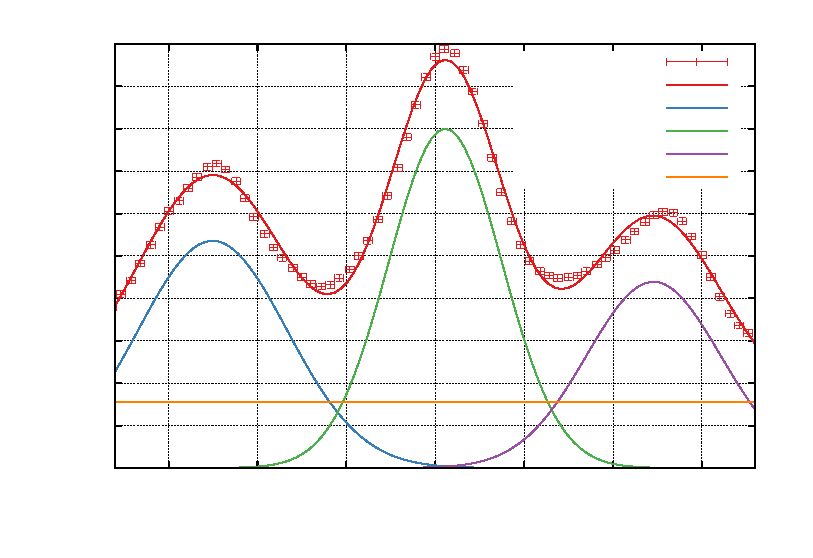
\includegraphics{./plots/zeemann_aufspaltung/b8-5}}%
    \gplfronttext
  \end{picture}%
\endgroup

	}
	\subcaption{}
\end{subfigure}
\\
\begin{subfigure}[l]{0.5\textwidth}
	\scalebox{0.75}{
	% GNUPLOT: LaTeX picture with Postscript
\begingroup
  \makeatletter
  \providecommand\color[2][]{%
    \GenericError{(gnuplot) \space\space\space\@spaces}{%
      Package color not loaded in conjunction with
      terminal option `colourtext'%
    }{See the gnuplot documentation for explanation.%
    }{Either use 'blacktext' in gnuplot or load the package
      color.sty in LaTeX.}%
    \renewcommand\color[2][]{}%
  }%
  \providecommand\includegraphics[2][]{%
    \GenericError{(gnuplot) \space\space\space\@spaces}{%
      Package graphicx or graphics not loaded%
    }{See the gnuplot documentation for explanation.%
    }{The gnuplot epslatex terminal needs graphicx.sty or graphics.sty.}%
    \renewcommand\includegraphics[2][]{}%
  }%
  \providecommand\rotatebox[2]{#2}%
  \@ifundefined{ifGPcolor}{%
    \newif\ifGPcolor
    \GPcolortrue
  }{}%
  \@ifundefined{ifGPblacktext}{%
    \newif\ifGPblacktext
    \GPblacktexttrue
  }{}%
  % define a \g@addto@macro without @ in the name:
  \let\gplgaddtomacro\g@addto@macro
  % define empty templates for all commands taking text:
  \gdef\gplbacktext{}%
  \gdef\gplfronttext{}%
  \makeatother
  \ifGPblacktext
    % no textcolor at all
    \def\colorrgb#1{}%
    \def\colorgray#1{}%
  \else
    % gray or color?
    \ifGPcolor
      \def\colorrgb#1{\color[rgb]{#1}}%
      \def\colorgray#1{\color[gray]{#1}}%
      \expandafter\def\csname LTw\endcsname{\color{white}}%
      \expandafter\def\csname LTb\endcsname{\color{black}}%
      \expandafter\def\csname LTa\endcsname{\color{black}}%
      \expandafter\def\csname LT0\endcsname{\color[rgb]{1,0,0}}%
      \expandafter\def\csname LT1\endcsname{\color[rgb]{0,1,0}}%
      \expandafter\def\csname LT2\endcsname{\color[rgb]{0,0,1}}%
      \expandafter\def\csname LT3\endcsname{\color[rgb]{1,0,1}}%
      \expandafter\def\csname LT4\endcsname{\color[rgb]{0,1,1}}%
      \expandafter\def\csname LT5\endcsname{\color[rgb]{1,1,0}}%
      \expandafter\def\csname LT6\endcsname{\color[rgb]{0,0,0}}%
      \expandafter\def\csname LT7\endcsname{\color[rgb]{1,0.3,0}}%
      \expandafter\def\csname LT8\endcsname{\color[rgb]{0.5,0.5,0.5}}%
    \else
      % gray
      \def\colorrgb#1{\color{black}}%
      \def\colorgray#1{\color[gray]{#1}}%
      \expandafter\def\csname LTw\endcsname{\color{white}}%
      \expandafter\def\csname LTb\endcsname{\color{black}}%
      \expandafter\def\csname LTa\endcsname{\color{black}}%
      \expandafter\def\csname LT0\endcsname{\color{black}}%
      \expandafter\def\csname LT1\endcsname{\color{black}}%
      \expandafter\def\csname LT2\endcsname{\color{black}}%
      \expandafter\def\csname LT3\endcsname{\color{black}}%
      \expandafter\def\csname LT4\endcsname{\color{black}}%
      \expandafter\def\csname LT5\endcsname{\color{black}}%
      \expandafter\def\csname LT6\endcsname{\color{black}}%
      \expandafter\def\csname LT7\endcsname{\color{black}}%
      \expandafter\def\csname LT8\endcsname{\color{black}}%
    \fi
  \fi
  \setlength{\unitlength}{0.0500bp}%
  \begin{picture}(7488.00,5040.00)%
    \gplgaddtomacro\gplbacktext{%
      \csname LTb\endcsname%
      \put(814,704){\makebox(0,0)[r]{\strut{} 0}}%
      \csname LTb\endcsname%
      \put(814,1383){\makebox(0,0)[r]{\strut{} 10}}%
      \csname LTb\endcsname%
      \put(814,2061){\makebox(0,0)[r]{\strut{} 20}}%
      \csname LTb\endcsname%
      \put(814,2740){\makebox(0,0)[r]{\strut{} 30}}%
      \csname LTb\endcsname%
      \put(814,3418){\makebox(0,0)[r]{\strut{} 40}}%
      \csname LTb\endcsname%
      \put(814,4097){\makebox(0,0)[r]{\strut{} 50}}%
      \csname LTb\endcsname%
      \put(814,4775){\makebox(0,0)[r]{\strut{} 60}}%
      \csname LTb\endcsname%
      \put(1458,484){\makebox(0,0){\strut{} 0.85}}%
      \csname LTb\endcsname%
      \put(2312,484){\makebox(0,0){\strut{} 0.9}}%
      \csname LTb\endcsname%
      \put(3165,484){\makebox(0,0){\strut{} 0.95}}%
      \csname LTb\endcsname%
      \put(4019,484){\makebox(0,0){\strut{} 1}}%
      \csname LTb\endcsname%
      \put(4872,484){\makebox(0,0){\strut{} 1.05}}%
      \csname LTb\endcsname%
      \put(5725,484){\makebox(0,0){\strut{} 1.1}}%
      \csname LTb\endcsname%
      \put(6579,484){\makebox(0,0){\strut{} 1.15}}%
      \put(176,2739){\rotatebox{-270}{\makebox(0,0){\strut{}Intensität $I$ / \si{\percent}}}}%
      \put(4018,154){\makebox(0,0){\strut{}Winkel $\alpha$ / \si{\degree}}}%
      \put(4018,4665){\makebox(0,0){\strut{}}}%
    }%
    \gplgaddtomacro\gplfronttext{%
      \csname LTb\endcsname%
      \put(6104,4602){\makebox(0,0)[r]{\strut{}Messwerte}}%
      \csname LTb\endcsname%
      \put(6104,4382){\makebox(0,0)[r]{\strut{}$\Sigma$}}%
      \csname LTb\endcsname%
      \put(6104,4162){\makebox(0,0)[r]{\strut{}$\mathcal{G}_1$}}%
      \csname LTb\endcsname%
      \put(6104,3942){\makebox(0,0)[r]{\strut{}$\mathcal{G}_2$}}%
      \csname LTb\endcsname%
      \put(6104,3722){\makebox(0,0)[r]{\strut{}$\mathcal{G}_3$}}%
      \csname LTb\endcsname%
      \put(6104,3502){\makebox(0,0)[r]{\strut{}$d$}}%
    }%
    \gplbacktext
    \put(0,0){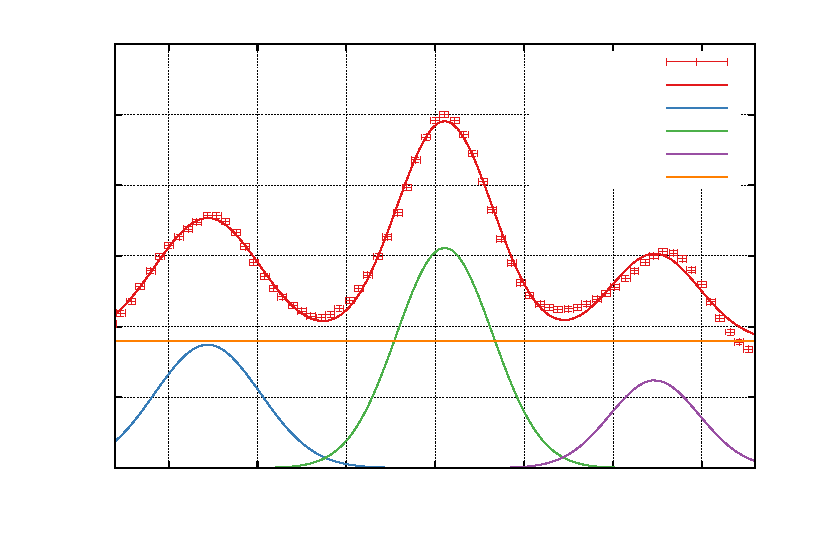
\includegraphics{./plots/zeemann_aufspaltung/b8-9}}%
    \gplfronttext
  \end{picture}%
\endgroup

	}
	\subcaption{}
\end{subfigure}
\caption{Magnetfeldaufspaltung Fits für \textbf{(a)} \SI{8}{\ampere}, \textbf{(b)} \SI{8.5}{\ampere}, \textbf{(c)}) \SI{8.9}{\ampere}}
\end{sidewaysfigure}

\end{appendix}

\end{document}
